\section{Data Far Sideband Studies}{}
\label{sec:sidebands}
This chapter documents the many far-sidebands made available to the analysis in April 2020 from the \npsel, \zpsel, and 2+ shower selections. Section~\ref{sec:sideband:definitions} introduces the sideband scheme adopted. Section~\ref{sec:sideband:recovery} and~\ref{sec:sideband:newcuts} presents recovery-algorithms and cut-updates implemented to the \npsel and \zpsel after gaining access to these sidebands. Sections~\ref{sec:sideband:1eNp} and~\ref{sec:sideband:1e0p} present results for the \npsel and \zpsel respectively showing in succession results from the 2+ shower, high-energy, and low-PID sidebands, as well as presenting a summary of time-stability plots and event-displays of selected events. 

The focus of this chapter is understanding the modeling of backgrounds and input variables on high-energy nue events in order to gain confidence in the analysis' maturity and readiness for final box opening. Results presented in this chapter show a very good level of agreement in detector and neutrino interaction modeling. A deficit in events observed after the final BDT-selection on the 2+ shower sideband for the \npsel is the most striking difference observed. The implications of this observation on the analysis are under assessment. Finally, while this section shows a highlight of far-sideband results, distributions for all relevant variables for the various sideband selections are included in appendix~\ref{app:datasidebandplotdump}.

\subsection{Sideband Definitions}
\label{sec:sideband:definitions}
The definition of sidebands of increasing sensitivity reflects the approach suggested by the oscillation conveners in \href{https://microboone-docdb.fnal.gov/cgi-bin/private/ShowDocument?docid=29203}{DocDB 29203}.
This scheme consists of identifying three regions of progressively lower energy and three regions of progressively higher event identification score.
This is shown schematically in the figure \ref{fig:sidebandsintro}.
The signal box is defined at low energy and high signal score.
The boxes adjacent to the signal one constitute the near sideband, whereas the furthest ones are identified as far sideband.
This system lets us approach the signal box in steps.
At each step, the low energy regions at different identification score allow the assessment of the simulation of the backgrounds, whereas the high identification score regions provides a pure set of \nuecc interactions.

The variable chosen to define a threshold on the reconstructed energy is that defined in Section \ref{sec:ereco} and used for the \npsel and \zpsel final energy spectra used to estimate the analysis sensitivity.
The identification score cuts are defined as combinations of the BDT scores with other box cuts, defined independently for each sideband.

\begin{figure}[H]
    \begin{center}
    \begin{subfigure}{0.5\textwidth}
    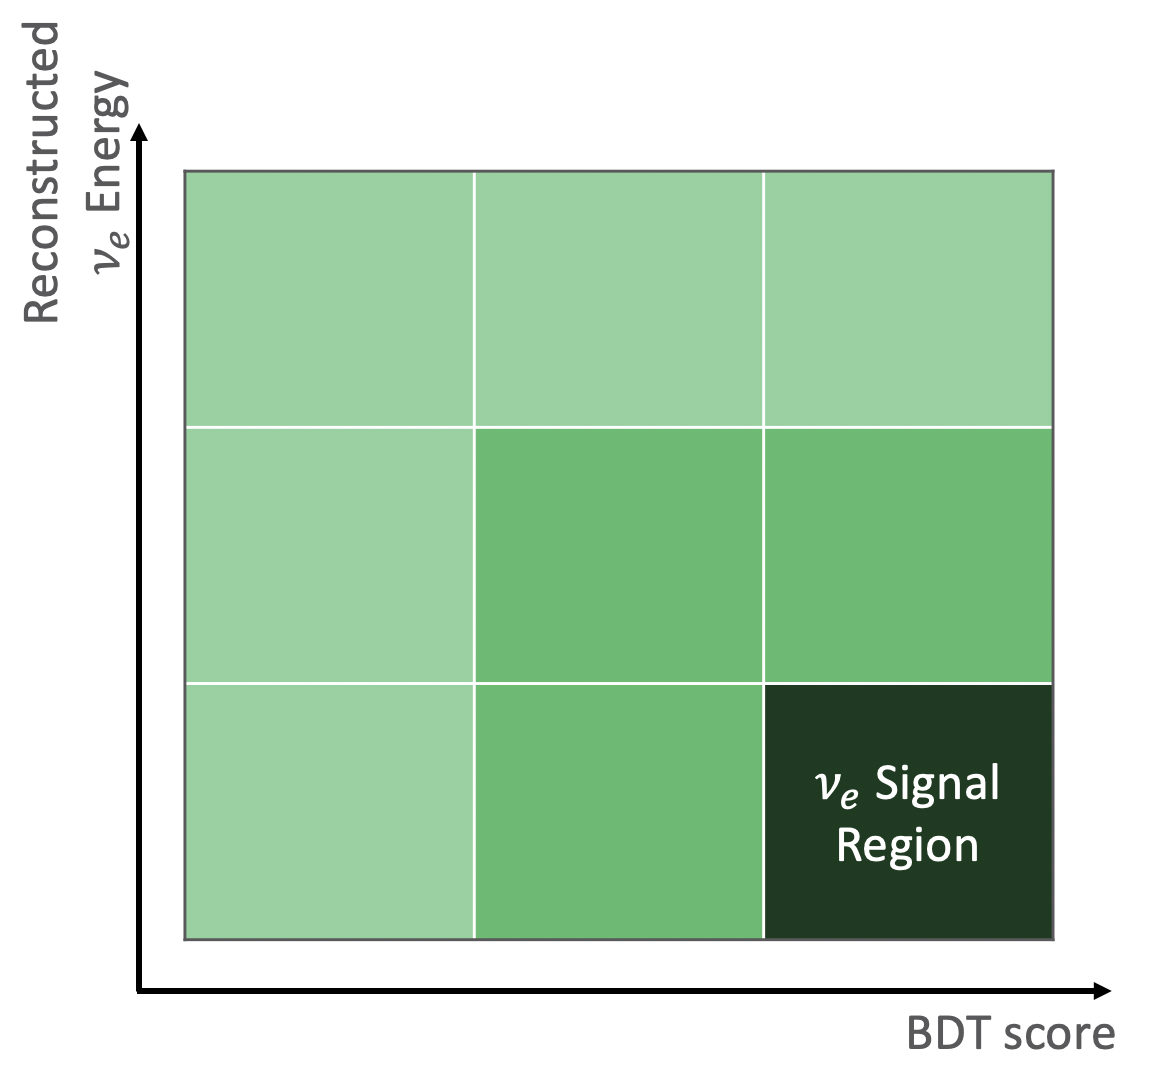
\includegraphics[width=0.8\textwidth]{Sidebands/Figures/SidebandDiagram.png}
    %\caption{\npsel Preselection}
    \end{subfigure}
    \caption{\label{fig:sidebandsintro} Schematic of the sideband structure.}
    \end{center}
\end{figure}
\begin{comment}
\begin{figure}[H]
    \centering
    \begin{subfigure}{0.48\textwidth}
    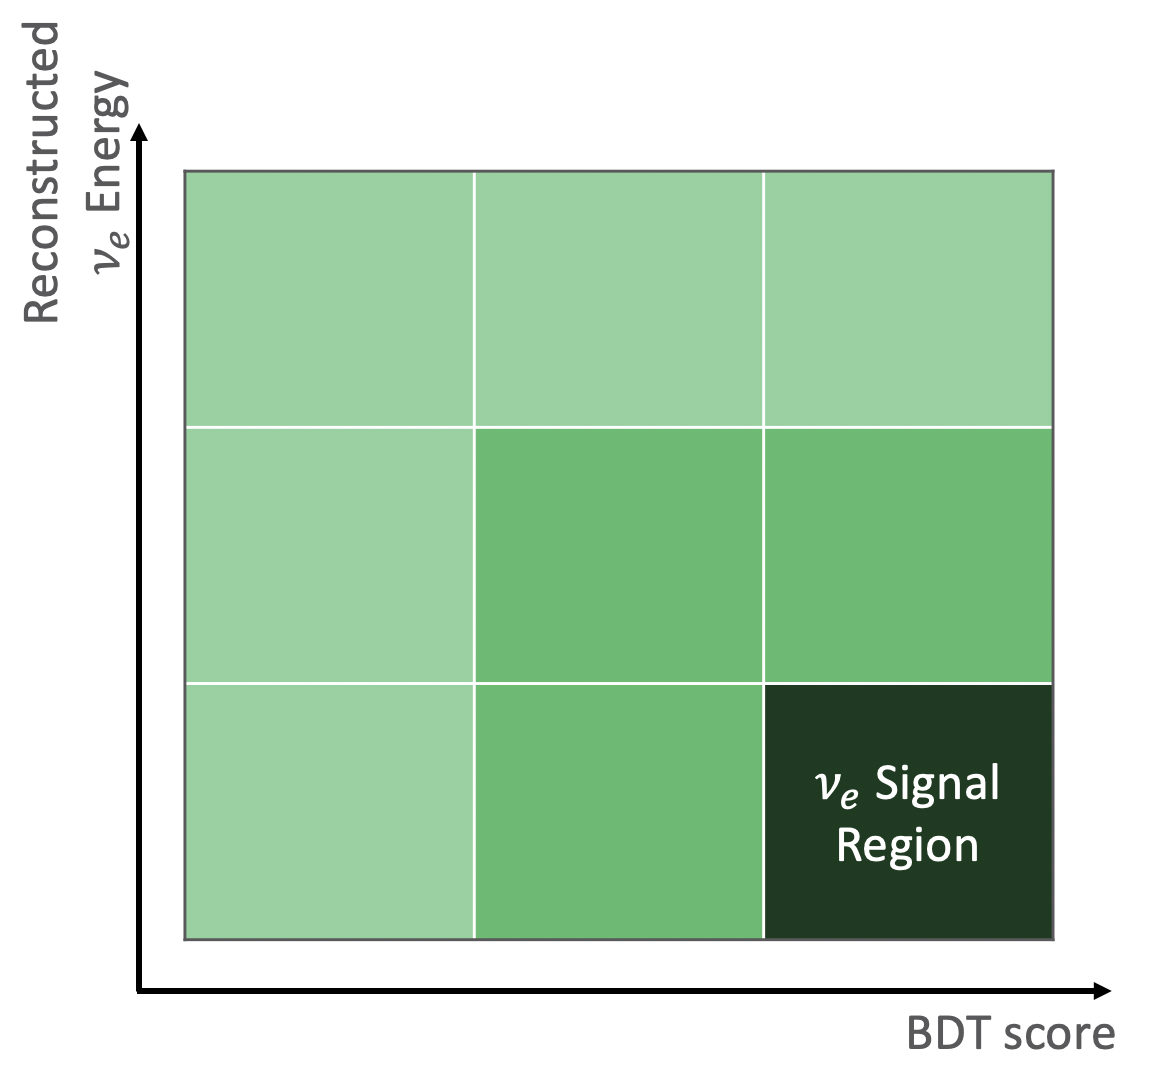
\includegraphics[width=0.8\textwidth]{Sidebands/Figures/SidebandDiagram.png}
    \caption{Schematic of the sideband structure.}
    \end{subfigure}
    \begin{subfigure}{0.48\textwidth}
    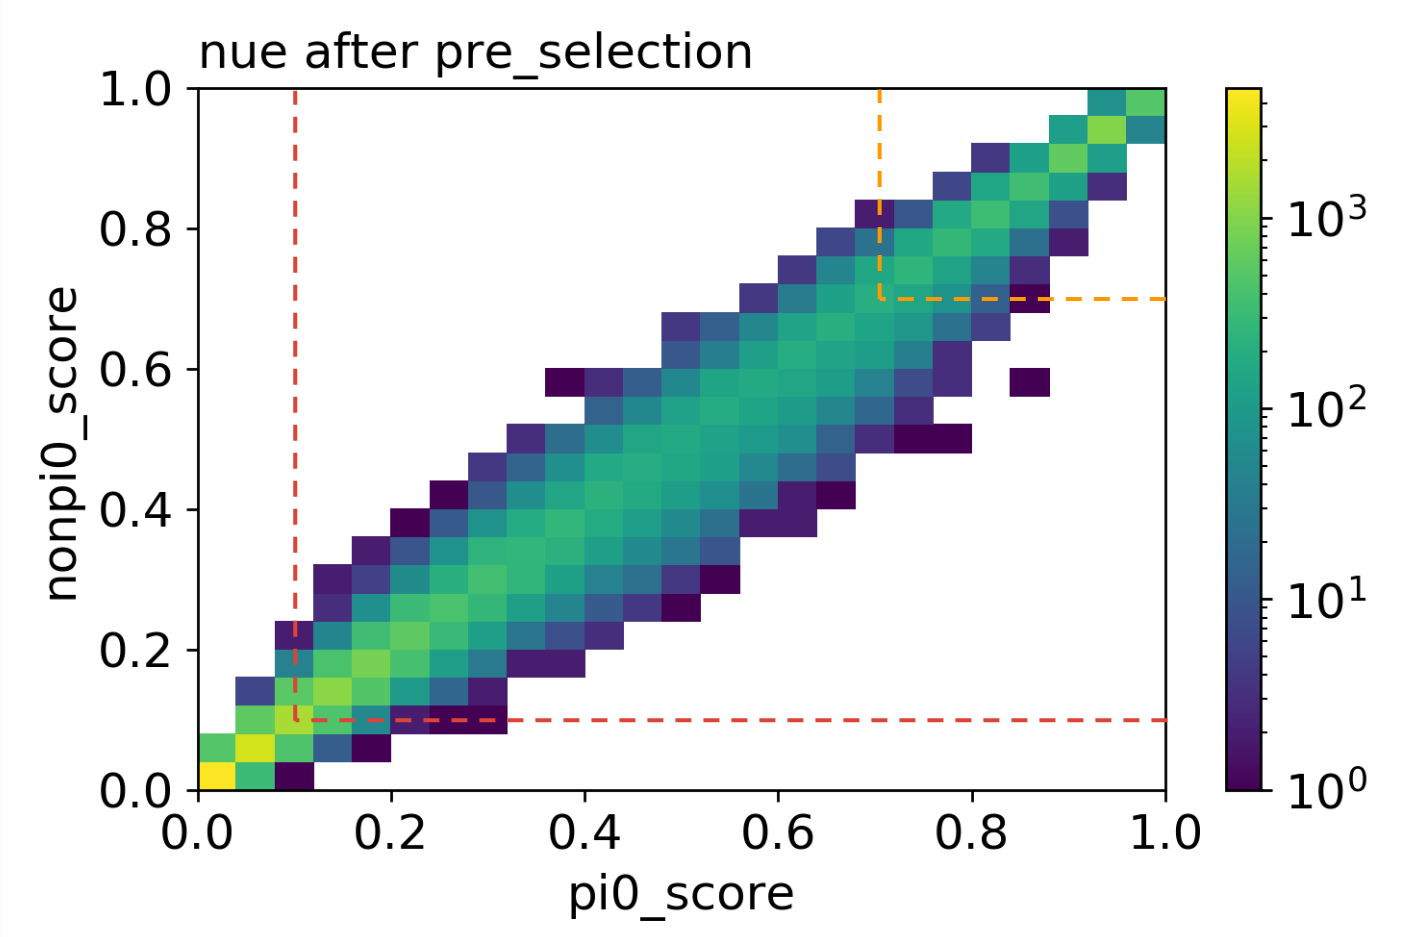
\includegraphics[width=0.8\textwidth]{Sidebands/Figures/1eNp/bdts_correlation.png}
    \caption{Correlation among the two 1eNp BDT scores for the \nue sample.}
    \end{subfigure}
    \caption{Introduction to the sideband strategy.} 
    \label{Schematic of the sideband structure.}
\end{figure}
\end{comment}

% \begin{figure}[h!]
% \centering
% \subfloat[Schematic of the sideband structure.] {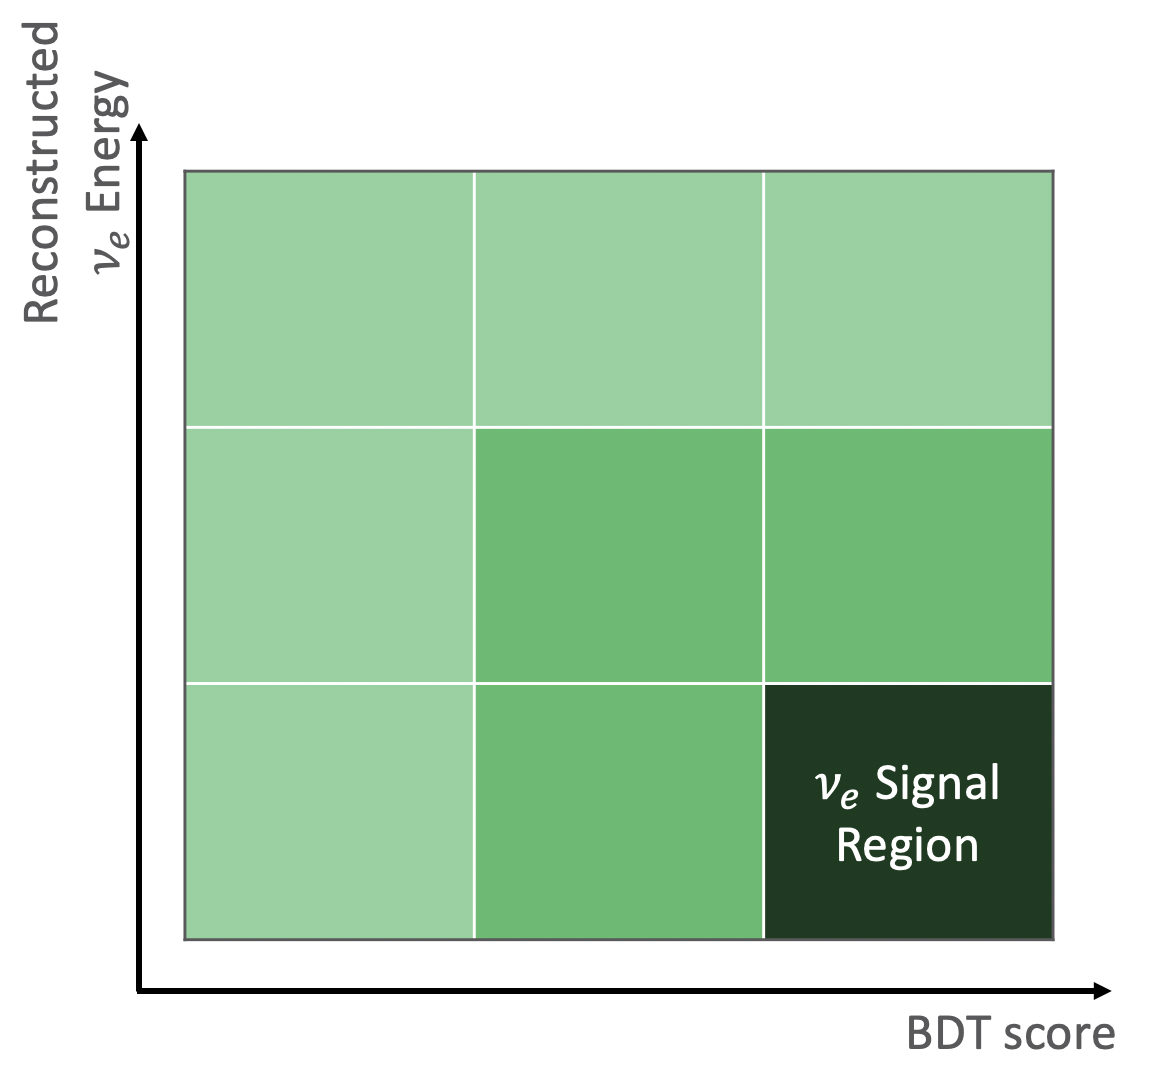
\includegraphics[width=0.48\textwidth]{Sidebands/Figures/SidebandDiagram.png}}\hfill
% \subfloat[Correlation among the two 1eNp BDT scores for the \nue sample.] {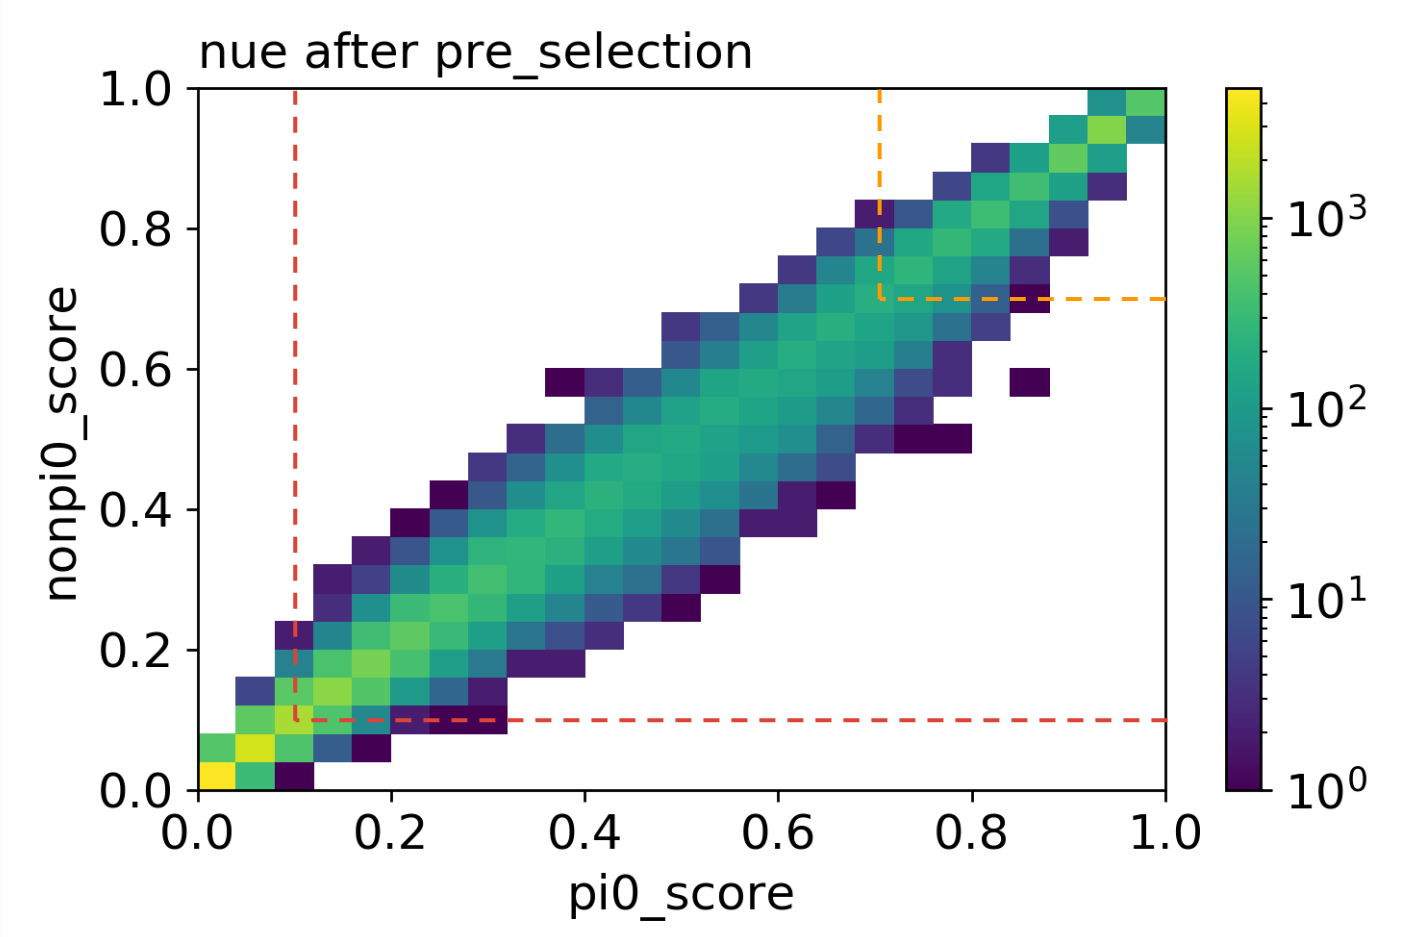
\includegraphics[width=0.8\textwidth]{Sidebands/Figures/1eNp/bdts_correlation.png}}
% \caption{Introduction to the sideband strategy.} 
% \label{fig:sidebands_and_bdt_correlations}
% \end{figure}

\subsubsection{\npsel sidebands}

For the \npsel sideband, the cuts on the reconstructed energy are defined as:
\begin{itemize}
    \item High energy: $0.85 ~\text{GeV} < E_{reco} < 2.05 ~\text{GeV}$
    \item Medium energy: $0.65 ~\text{GeV} < E_{reco} < 0.85 ~\text{GeV}$
    \item Low energy: $0.05 ~\text{GeV} < E_{reco} < 0.65 ~\text{GeV}$
\end{itemize}

Two BDTs are used to define the \npsel selection; one to identify $\pi_0$ backgrounds, and another to identify non-$\pi_0$ backgrounds. Cuts on both of these are made to define the event-ID sideband regions. 
%For the event selection definition, cuts are made on, the three regions are defined using the BDT scores as well a combination of preselection and loose selection cuts.
%The two BDT scores are very correlated, as shown in the right plot of figure \ref{fig:sidebands_and_bdt_correlations}, and thus the following strategy is adopted:
\begin{itemize}
    \item Low PID: pre-selection cuts, exactly one contained shower, and $0 < \pi_0~\text{score} < 0.1 ~\text{or}~ 0 < \text{non}~\pi_0~\text{score} < 0.1 $
    \item Medium PID: pre-selection cuts, exactly one contained shower, and $(0.1 < \pi_0~\text{score} < 0.67 ~\text{or}~ 0.1 < \text{non}~\pi_0~\text{score} < 0.7) ~\text{and}~  (\pi_0~\text{score} > 0.1) ~\text{and}~ (\text{non}~\pi_0~\text{score} > 0.1)$
    \item High PID (signal region): loose-selection cuts, and $ \pi_0~\text{score} > 0.67 ~\text{and}~ \text{non}~\pi_0~\text{score} > 0.7 $
\end{itemize}
For the low and medium event ID the loose selection cuts have been relaxed to the pre-selection cuts plus the requirement of exactly one shower contained.
This cut relaxation ensures larger statistics in the sideband distributions.
Requiring a single contained shower let us use the sample with two or more contained showers as an additional sideband, which is primarily events with two showers that are produced by \pizero decays.

\subsubsection{\zpsel sidebands}
A similar procedure was followed to determine a set of sidebands for the \zpsel channel. The cuts on the reconstructed visible energy are defined as:

\begin{itemize}
    \item High energy: $E_{reco} > 0.9 ~\text{GeV}$
    \item Medium energy: $0.65 ~\text{GeV} < E_{reco} < 0.9 ~\text{GeV}$
    \item Low energy: $E_{reco} < 0.65 ~\text{GeV}$
\end{itemize}

The \zpsel channel uses a single BDT for background discrimination. This BDT assigns a score depending on if the event is classified as signal-like (BDT score near 1) or background-like (BDT score near 0). Thresholds are defined below:

\begin{itemize}
    \item Low PID: BDT score $<$ 0.4
    \item Medium PID: 0.4 $<$ BDT score $<$ 0.72
    \item High PID (signal region): BDT score $>$ 0.72
\end{itemize}

\subsubsection{Two+ showers sideband}
An additional sideband enriched of events with two or more showers has been studied.
This sideband does not follow the scheme previously described, and it is complementary to the previous series of sidebands.
This additional sideband is particularly useful to study the \pizero background following a similar selection approach used in the \npsel and \zpsel selections, and thus able to test data-MC agreement for signal-like $\pi^0$ backgrounds.
This sideband is defined by imposing the \nue pre-selection cuts, with no requirement on the number of tracks, and requiring at least two showers contained.
As no requirement on the number of tracks is applied, this sideband is useful for both the \nueccnopinp and \nueccnopinop selections.
While a \pizero selection has been developed as part of the PeLEE analysis, providing several thousand \pizero events for various analysis validations, this sideband specifically addresses the modelling of background events that fall close to the signal box as defined by the PID cuts, making this a valuable control sample.


\subsection{Recovery Algorithms for Reconstruction Failures}
\label{sec:sideband:recovery}
The reconstruction of \npsel events can be impacted by a variety of failure modes; some of them were investigated in the past but not addressed as they were not deemed to be of primary importance for a low-energy analysis (see e.g. DocDB 24172). The analysis of high energy sideband data led to the identification of a few failure modes that lead to mis-reconstruction effects that can be recovered at analysis stage. Recovering such events does not require a change in the selection criteria, but rather a re-interpretation of the events motivated by the correction of the reconstruction failures that are identified. Such recovery algorithms are applied to events in the \npsel to both to data and MC from all data taking periods. Further documentation on the recovery algorithms described here is available in \href{https://microboone-docdb.fnal.gov/cgi-bin/private/RetrieveFile?docid=31586&filename=failure-modes-recovery-algos-final-update.pdf&version=1}{DocDB 31586}.

We developed four recovery algorithms:
\begin{enumerate}
    \item {\bf Shower splitting}. Part of the electron shower is identified as a separate reconstructed shower. This pathology causes \npsel events to migrate from the 1-shower signal region to the 2-shower sideband. These events are identified by checking that the second shower is within the cone of the leading shower and at more than 60 cm from the leading track start; the leading shower is required to pass some shower identification requirements. The event reinterpretation requires updating the variables \texttt{subcluster}, \texttt{shrmoliereavg}, and the number of showers \texttt{n\_showers\_contained}. Figure~\ref{fig:recoveryalgos:split} shows an example event affected by this failure mode.
    \item {\bf Spurious leading track}. The failure in this case is that the leading track, which we consider a proton candidate, is actually spurious or unrelated to the neutrino interaction. This pathology leads to a large distance between the track and shower start points and typically to fail the proton identification. The identification criteria relies on the track start point to be more than 30 cm away from the neutrino vertex. The recovery of these events implies that all variables related to the track need to re-defined based the 2nd leading track; the contribution of the spurious track needs also to be removed from the energy calculation. Figure~\ref{fig:recoveryalgos:spurious} shows an example event affected by this failure mode.
    \item {\bf Shower start as track}. In these events, the electron shower is split in two separate objects: the initial, track-like segment is reconstructed as a (sub-leading) track, while the downstream "showery" part is a shower. The identification relies on the fact that the directions of the sub-leading track and of the shower are aligned. Additionally, the start point of the sub-leading track must be closer to the start point of the leading track than to the shower start point. Recovering these events requires taking the information about the shower start from the sub-leading shower and merging information of the sub-leading track into the main shower for the variables related to the shower development.
    \item {\bf Proton as shower}. Here the pathology is caused by protons connected to the neutrino interaction vertex which are reconstructed as a showers. These event moves into the 2-shower sideband. This failure is identified by requiring the "proton shower" to be close the leading track, to have a small number of sub-clusters, and to have a proton-like PID; the numerical values of these cuts are inspired by the loose selection. The event re-interpretation requires redefining the track and shower counts, as well as the energy variables.
\end{enumerate}

\begin{figure}[H]
    \centering
    \begin{subfigure}{0.30\textwidth}
    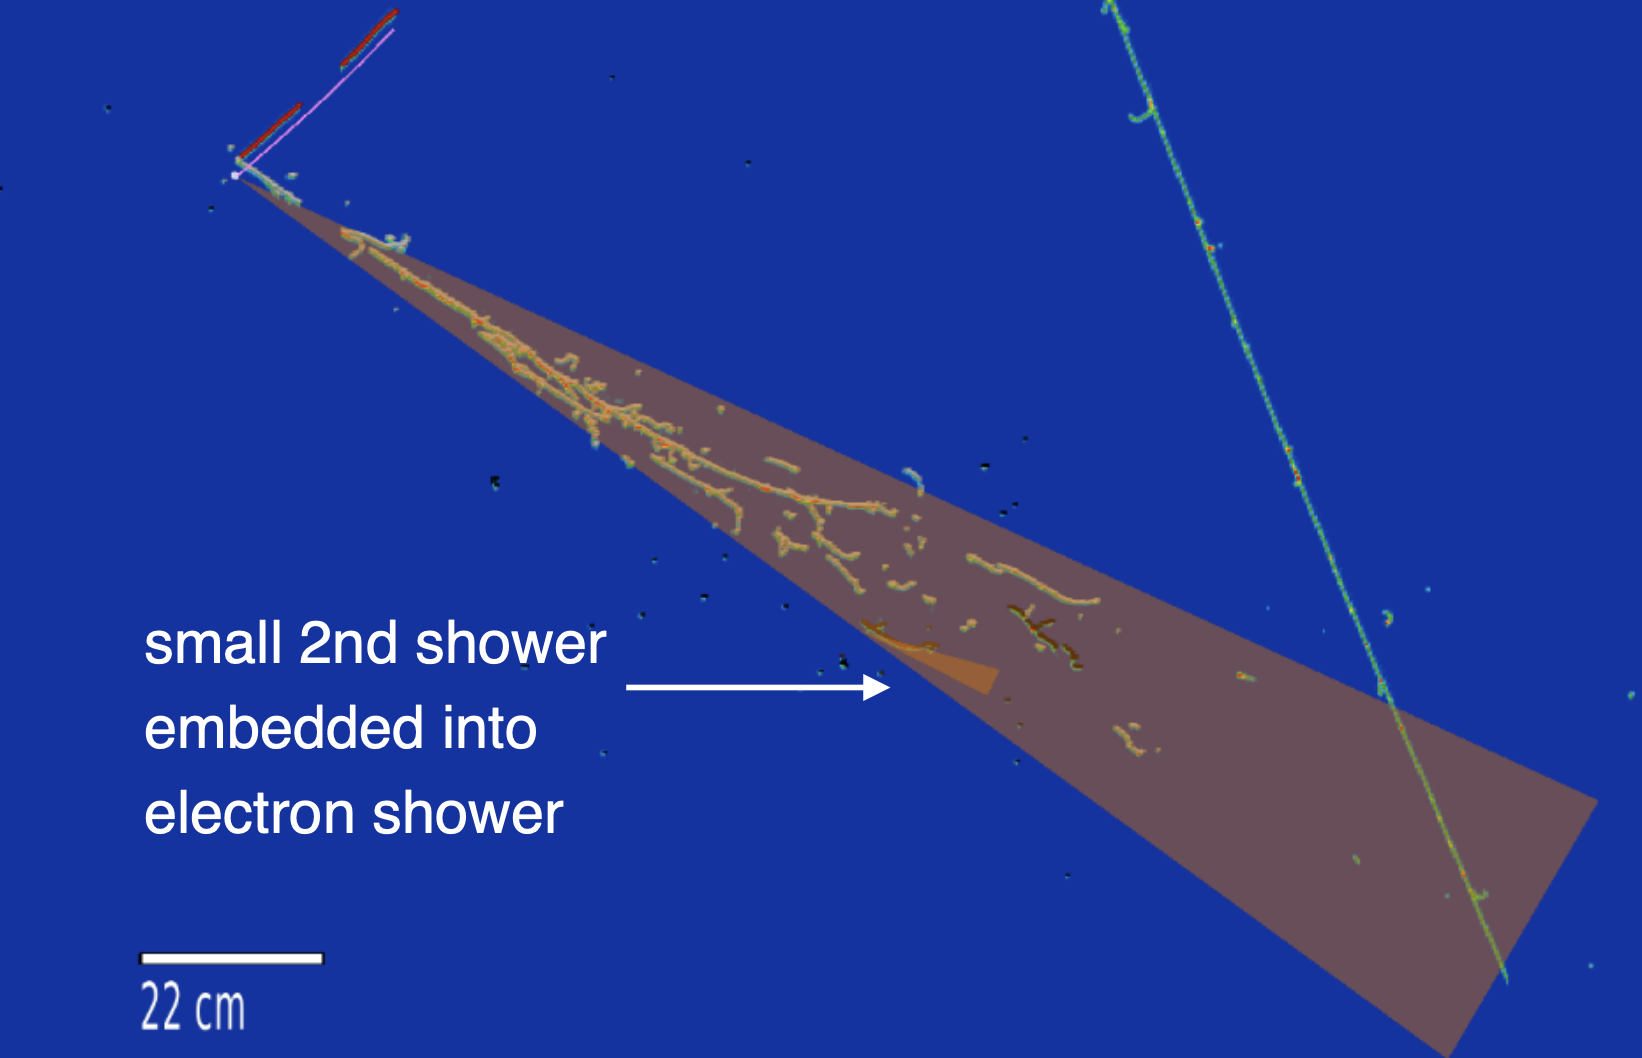
\includegraphics[width=1.00\textwidth]{Sidebands/Figures/CutUpdates/split-shower.png}
    \caption{\label{fig:recoveryalgos:split}Shower splitting.}
    \end{subfigure}
    \begin{subfigure}{0.40\textwidth}
    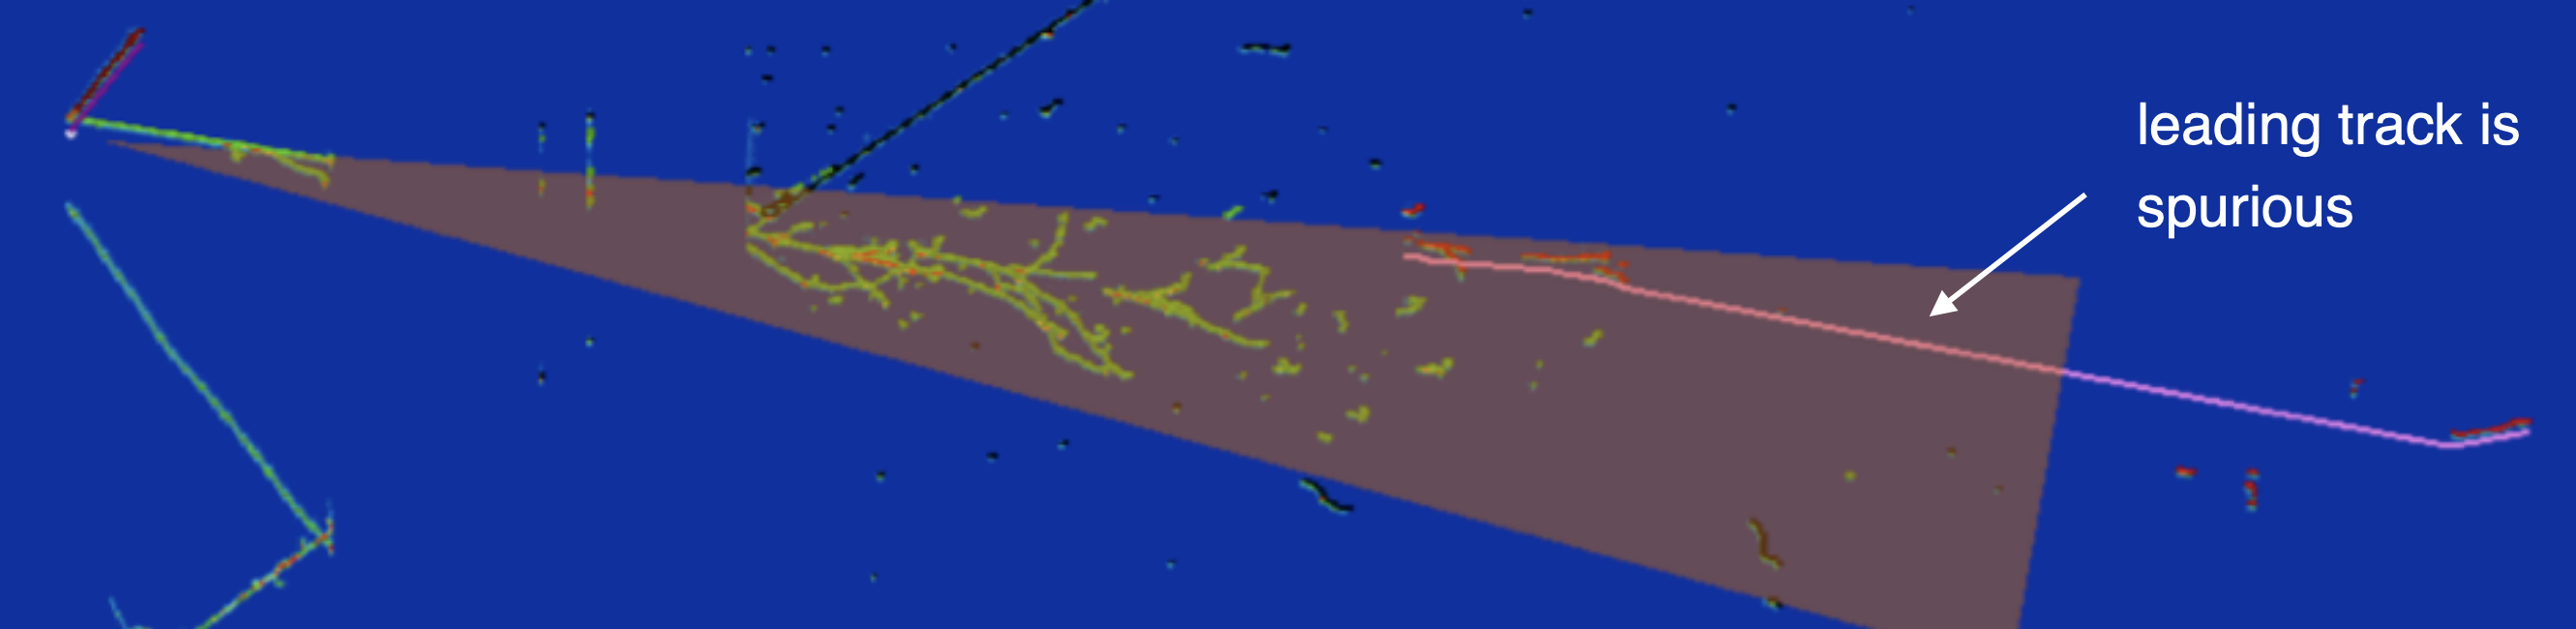
\includegraphics[width=1.00\textwidth]{Sidebands/Figures/CutUpdates/spurious-track.png}
    \caption{\label{fig:recoveryalgos:spurious}Spurious leading track.}
    \end{subfigure} \\
    \begin{subfigure}{0.35\textwidth}
    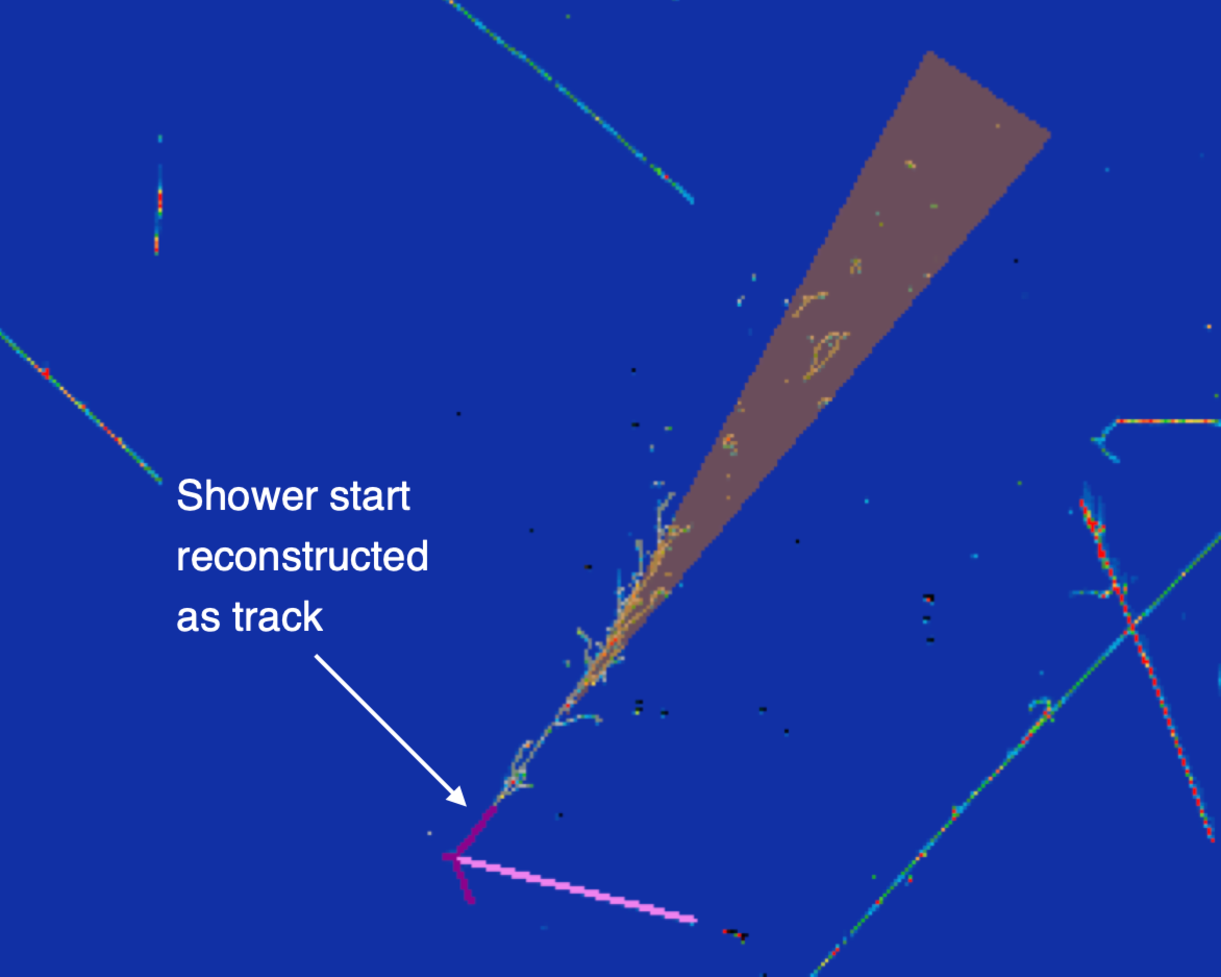
\includegraphics[width=1.00\textwidth]{Sidebands/Figures/CutUpdates/shr-start-as-track.pdf}
    \caption{\label{fig:recoveryalgos:split}Shower start as track.}
    \end{subfigure}
    \begin{subfigure}{0.35\textwidth}
    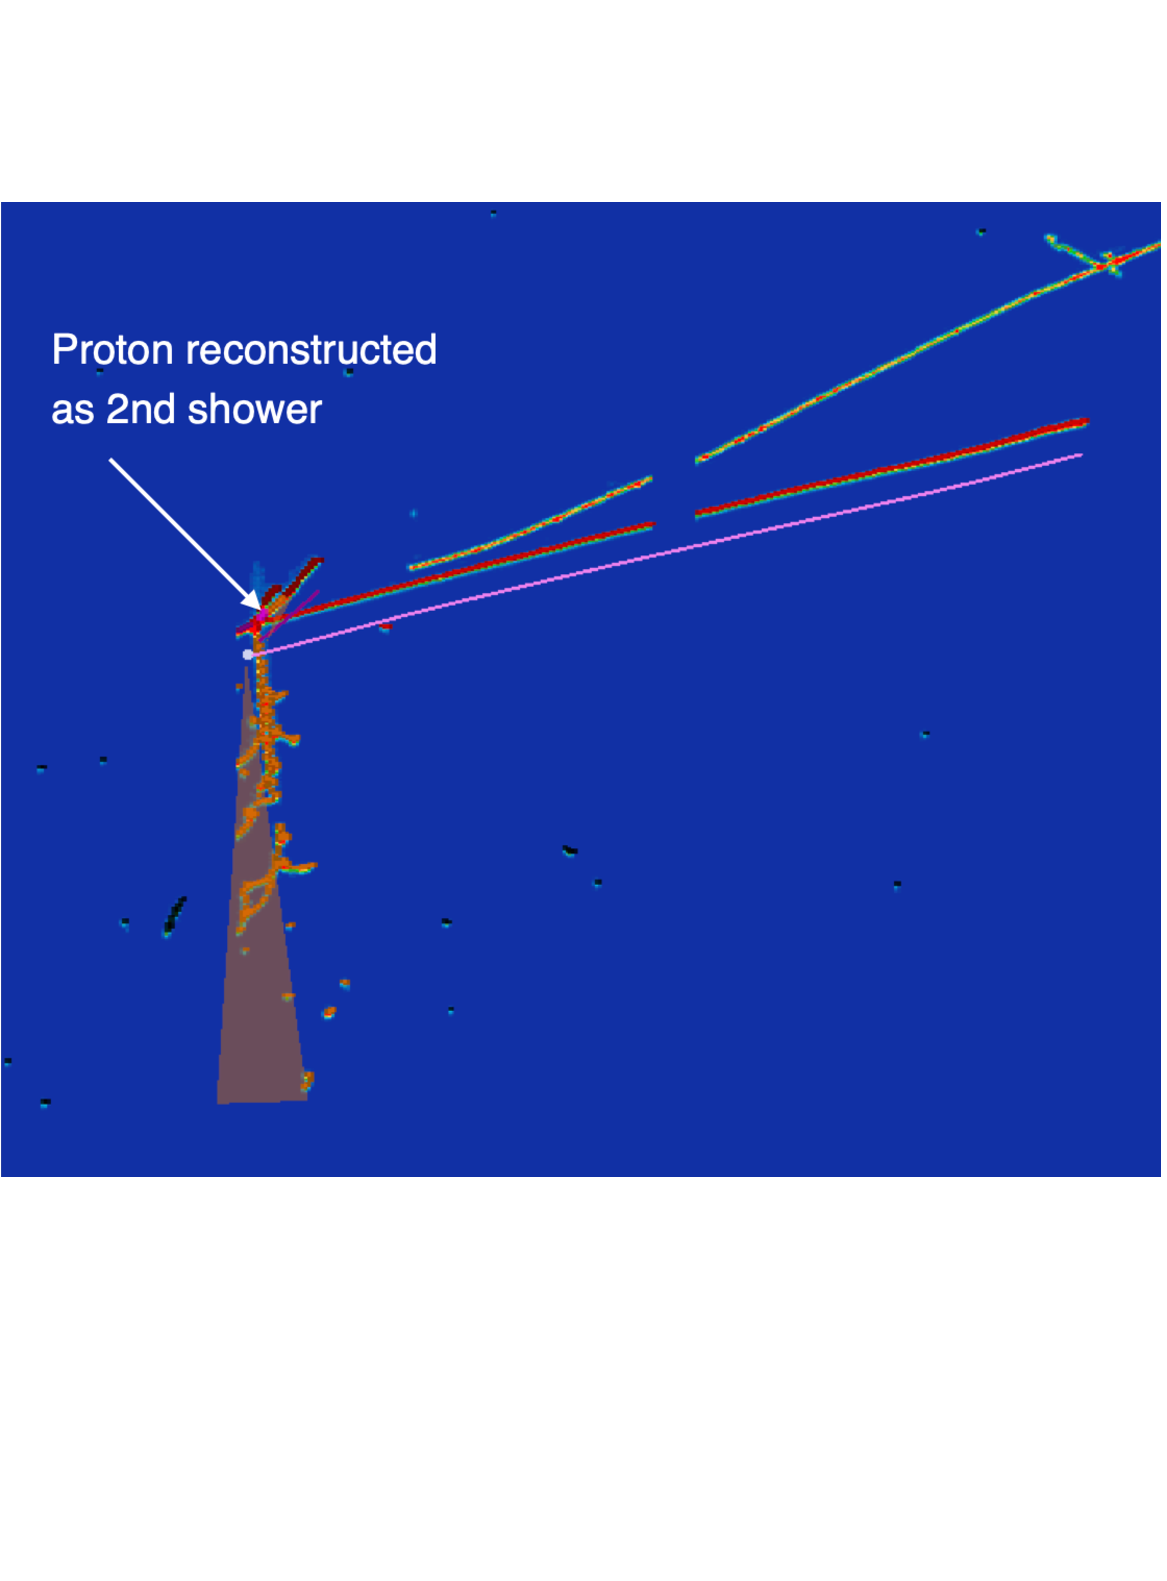
\includegraphics[width=1.00\textwidth]{Sidebands/Figures/CutUpdates/proton-as-shower.pdf}
    \caption{\label{fig:recoveryalgos:spurious}Proton as shower.}
    \end{subfigure}
    \caption{Examples of reconstruction failure modes targeted by recovery algorithms.}
    \label{fig:recoveryalgos}
\end{figure}

We observe an overall failure rate comparable between data and MC, both integrated over all run periods and looking separately into each run period (Fig.~\ref{failurerate}). However, the failures and subsequent recovery have a larger impact on Run3, where the number of events at high energy doubles from five to ten after including the recovery algorithms (Fig.~\ref{run3recovery}). Overall, the recovery algorithms add about 1/3 of the events at high energy, so their contribution is significant in this region. The failure mode that happens more frequently in \npsel events is the first, shower-splitting. Out of the 9 events recovered in the high-energy sideband after BDT selection, 7 of them are due to this mode. 

\begin{figure}[H]
    \centering
    \begin{subfigure}{0.35\textwidth}
    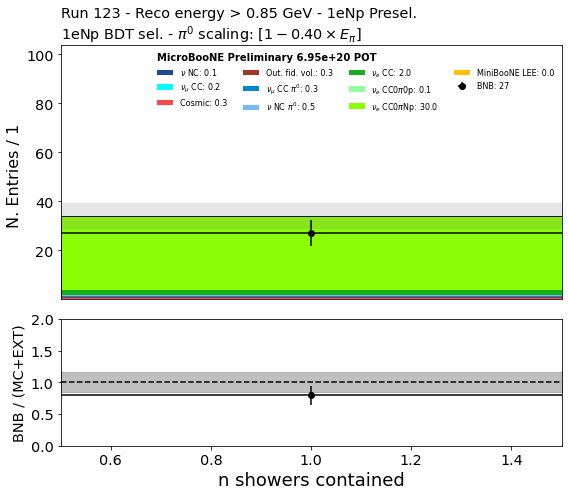
\includegraphics[width=1.00\textwidth]{Sidebands/Figures/CutUpdates/norecovery-allruns.png}
    \caption{No recovery, all runs.}
    \end{subfigure}
    \begin{subfigure}{0.35\textwidth}
    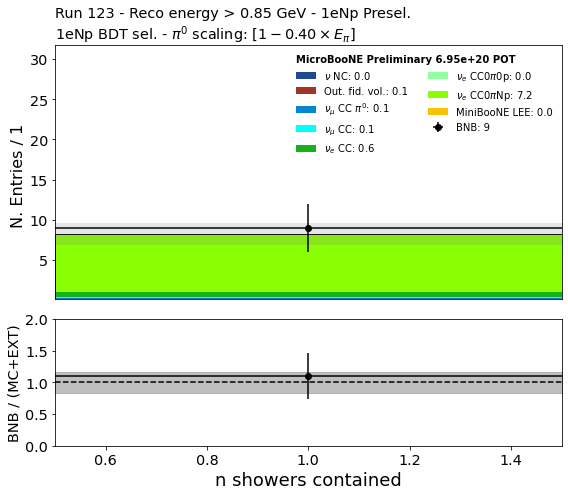
\includegraphics[width=1.00\textwidth]{Sidebands/Figures/CutUpdates/recovery-allruns.png}
    \caption{Recovery only, all runs.}
    \end{subfigure} \\
    \begin{subfigure}{0.35\textwidth}
    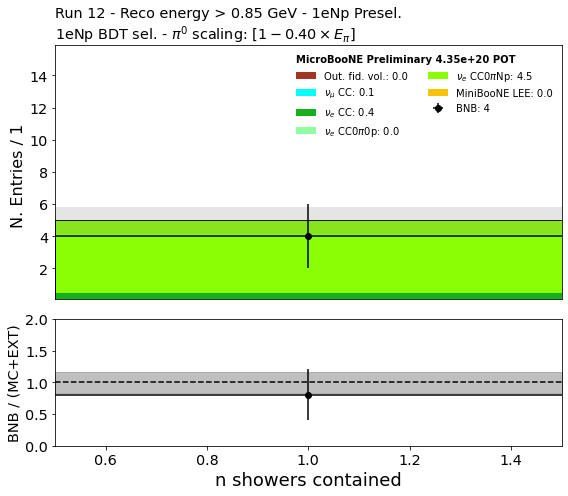
\includegraphics[width=1.00\textwidth]{Sidebands/Figures/CutUpdates/recovery-runs12.png}
    \caption{Recovery only, run 1+2.}
    \end{subfigure}
    \begin{subfigure}{0.35\textwidth}
    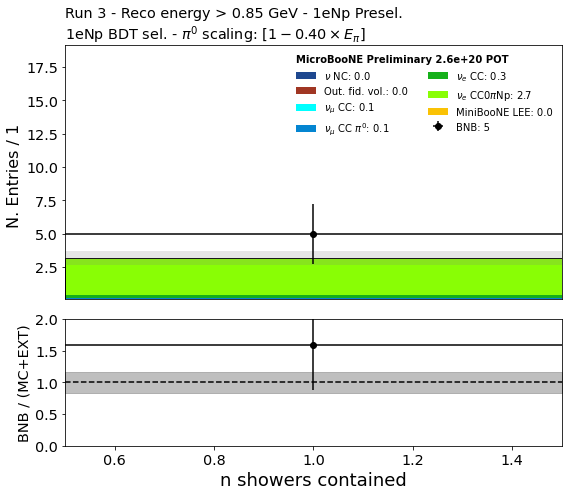
\includegraphics[width=1.00\textwidth]{Sidebands/Figures/CutUpdates/recovery-runs3.png}
    \caption{Recovery only, run 3.}
    \end{subfigure}
    \caption{Failure rate in data and MC, broken down in different data taking periods.}
    \label{failurerate}
\end{figure}

\begin{figure}[H]
    \centering
    \begin{subfigure}{0.35\textwidth}
    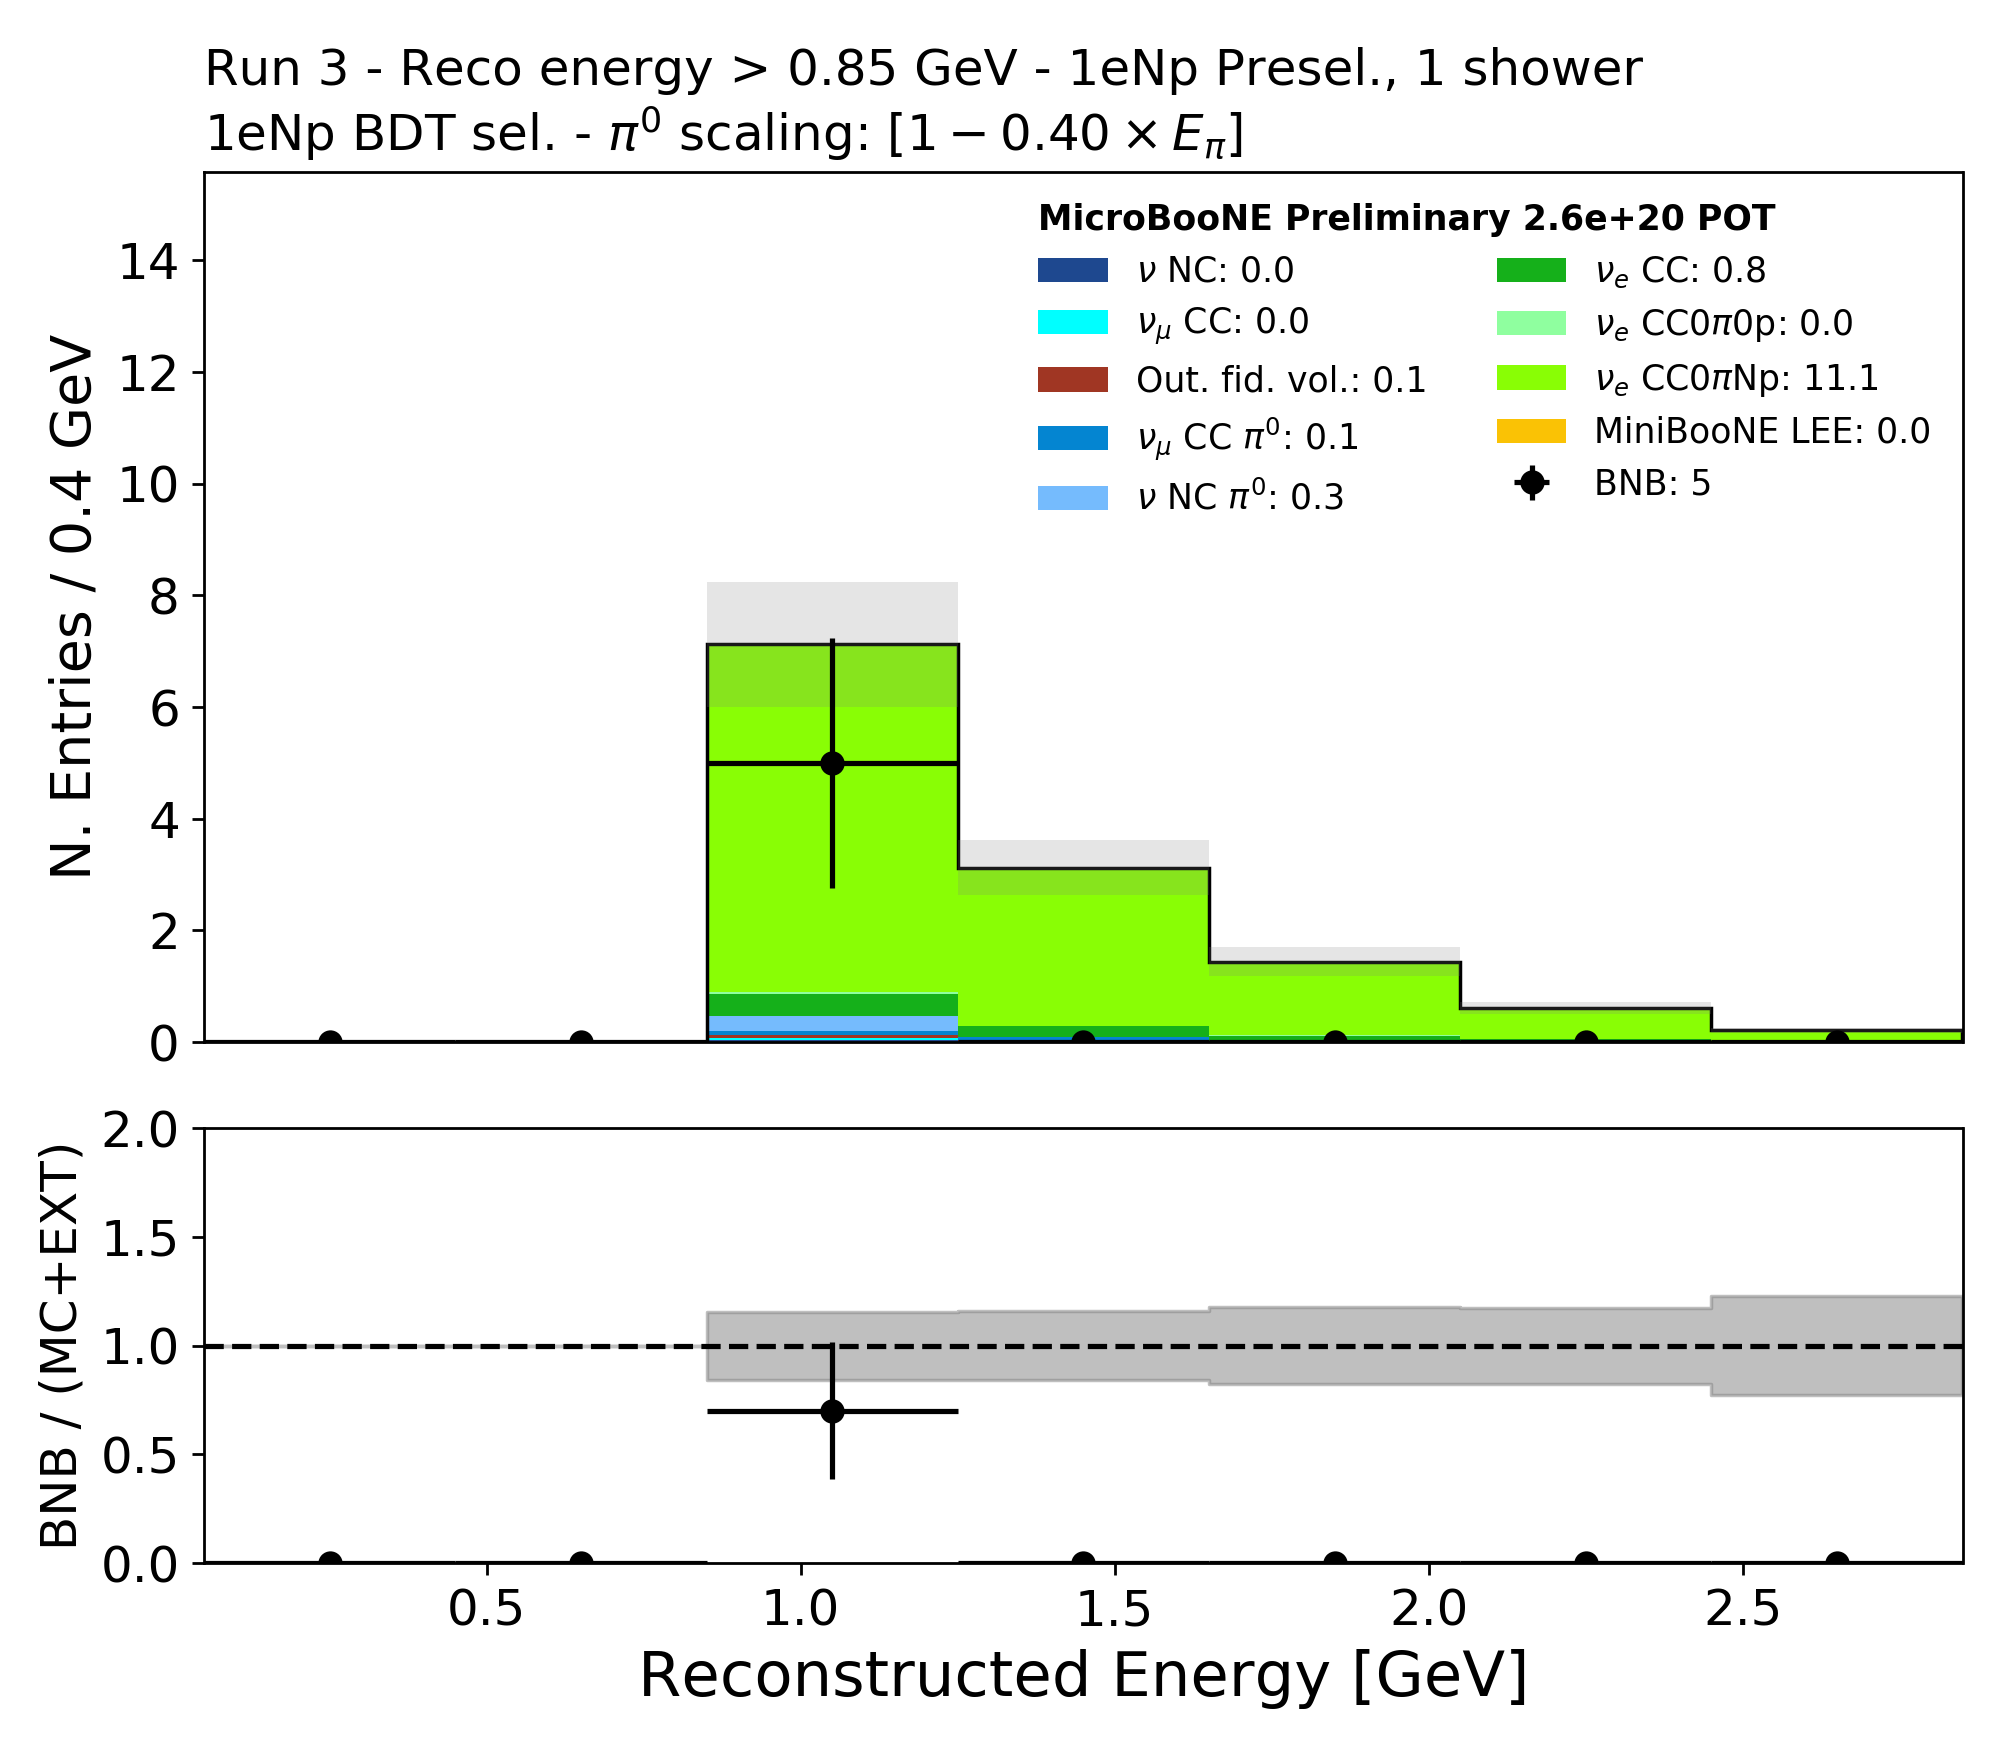
\includegraphics[width=1.00\textwidth]{Sidebands/Figures/CutUpdates/reco_e_coarse_run3_norecovery.png}
    \caption{No recovery, run 3.}
    \end{subfigure}
    \begin{subfigure}{0.35\textwidth}
    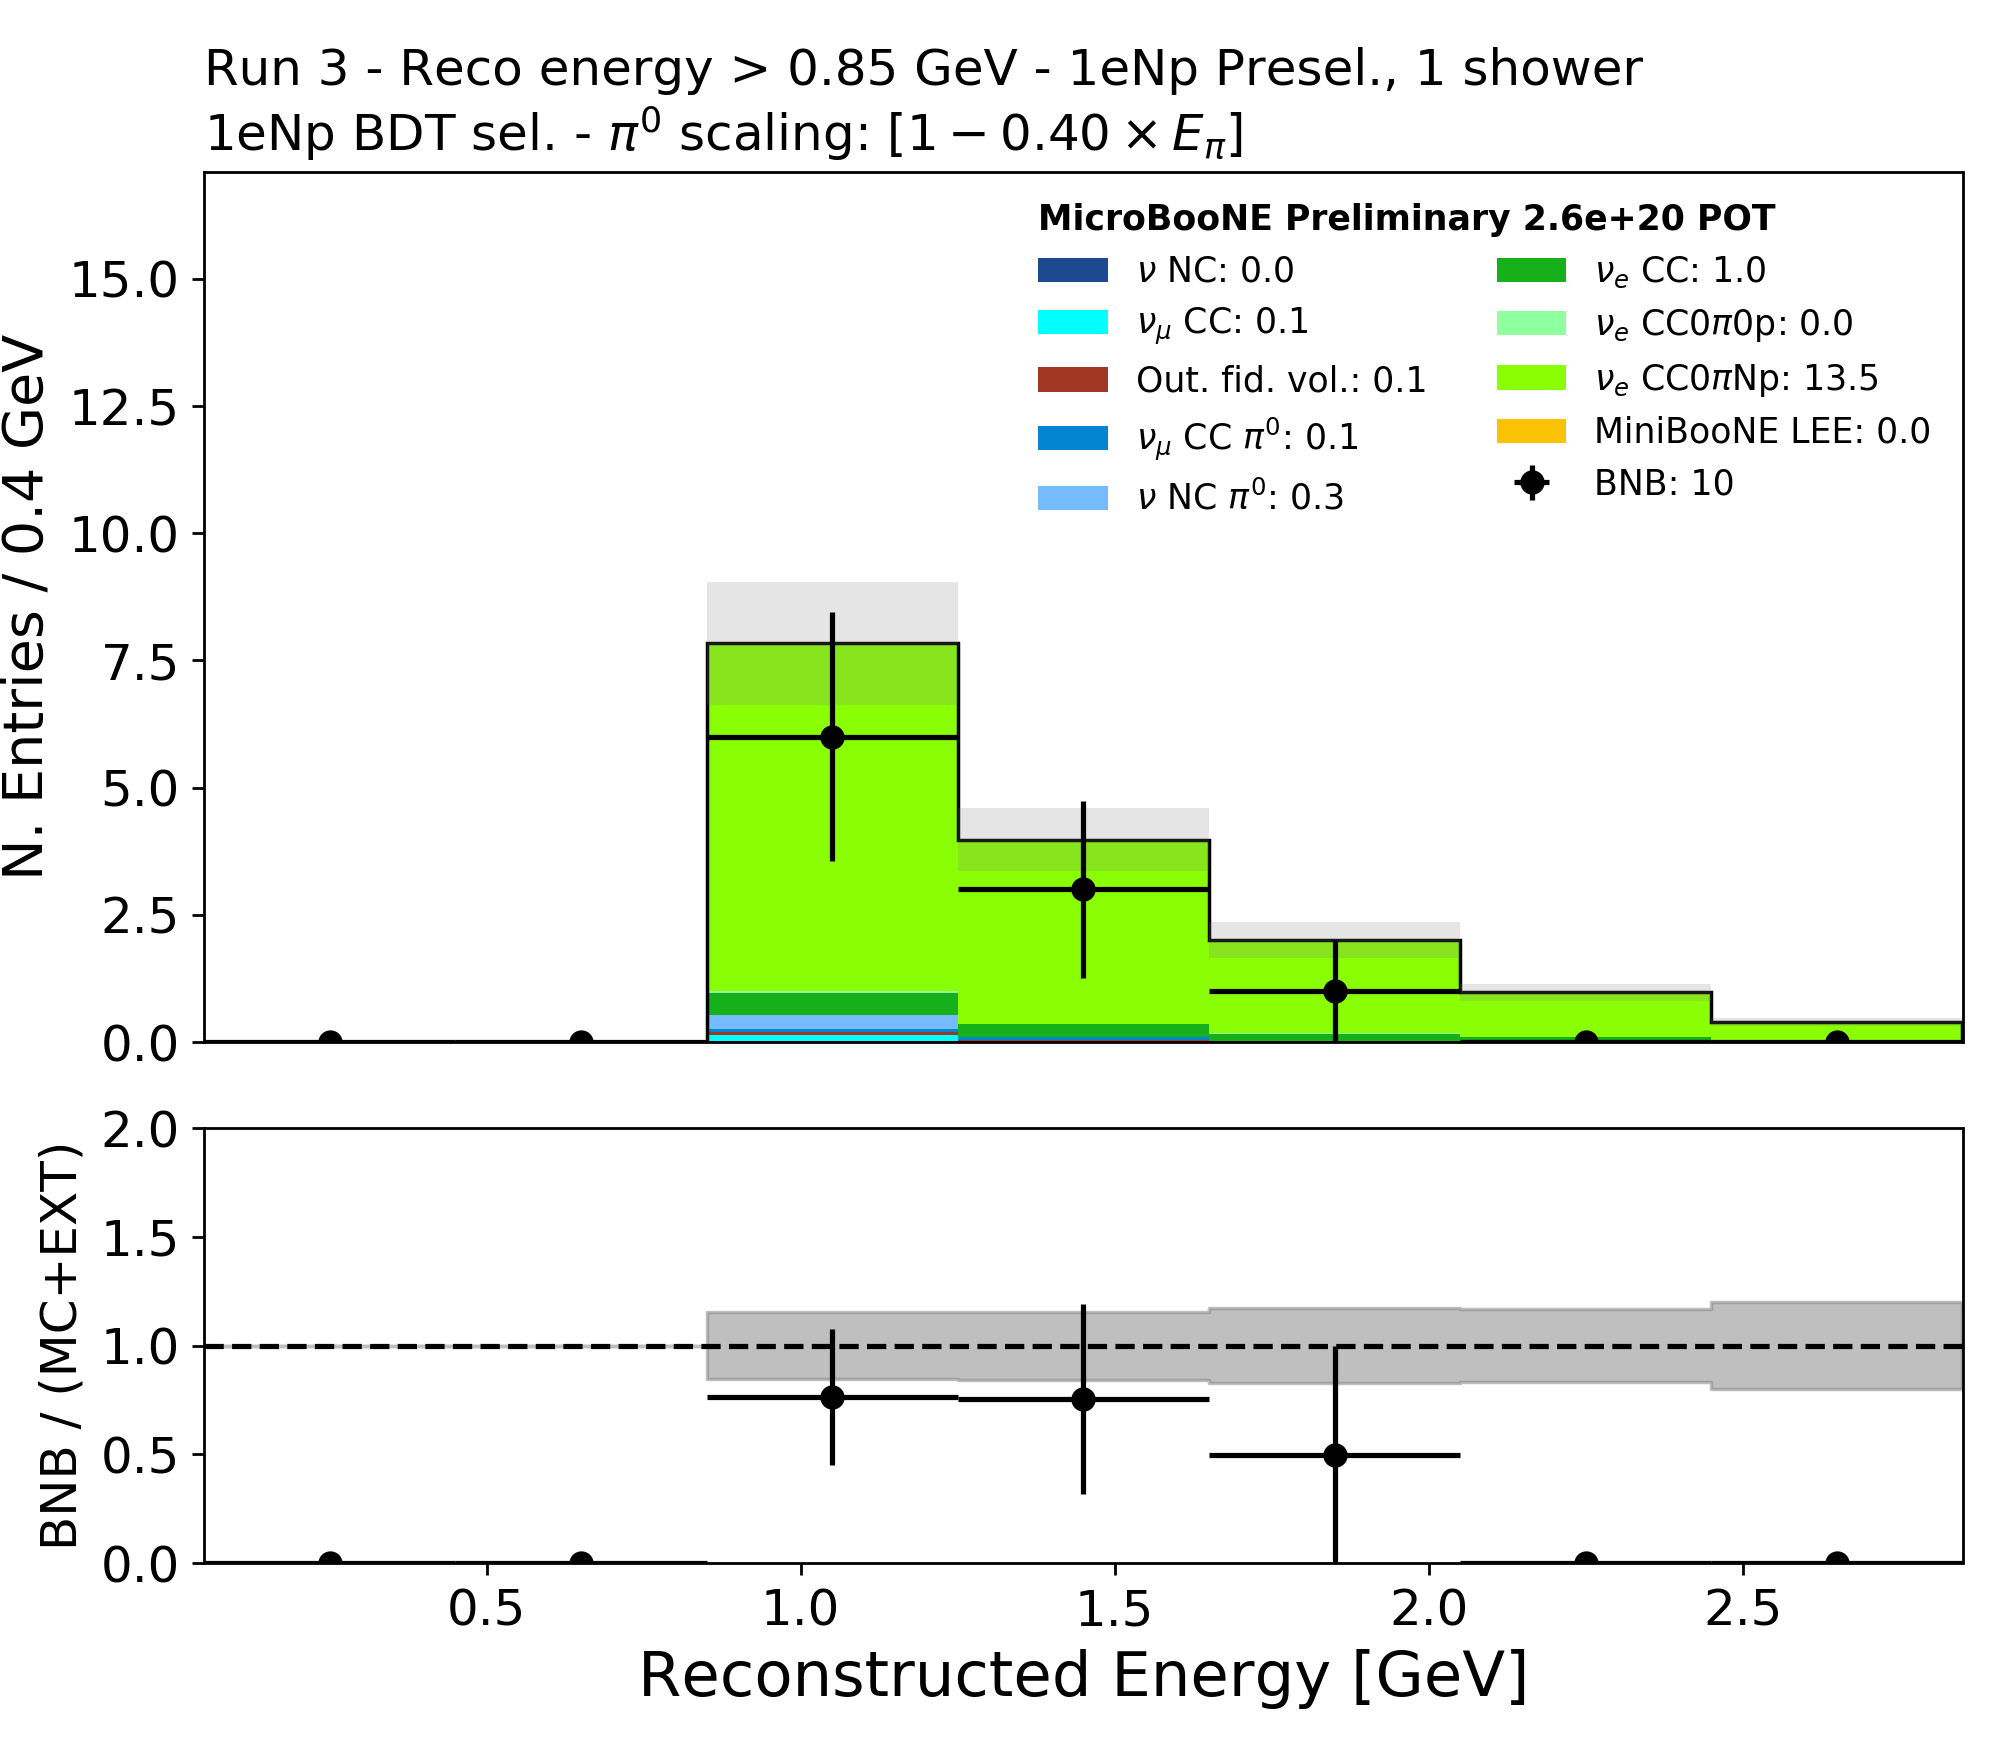
\includegraphics[width=1.00\textwidth]{Sidebands/Figures/CutUpdates/reco_e_coarse_run3_recovery.png}
    \caption{With recovery, run 3.}
    \end{subfigure}
    \caption{Effect of recovery algorithms in run 3 high energy \npsel data after BDT selection.}
    \label{run3recovery}
\end{figure}

The recovery algorithms are applied in the analysis of the \npsel data sidebands. They will also be included when looking into the near-sideband and the signal box, but their contribution is expected to be negligible; the main reason is that the dominant failure mode (shower splitting) affects high-energy electron showers only. Fig.~\ref{shrsplt-rate-vs-recoe} shows the expected rate of events migrating in the signal selection as a consequence of applying the shower splitting recovery algorithm. The recovery is expected to introduce less than one new event for the full Run 1-3 dataset below 1 GeV of reconstructed energy.

\begin{figure}[H]
    \centering
    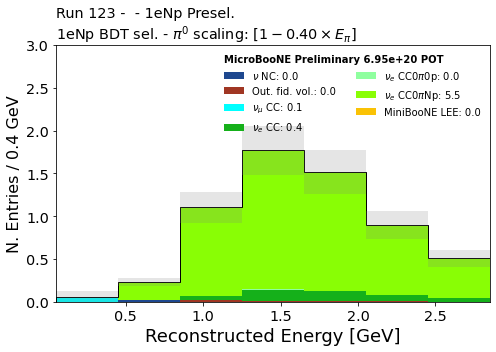
\includegraphics[width=0.40\textwidth]{Sidebands/Figures/CutUpdates/shrsplt-rate-vs-recoe.png}
    \caption{Expected rate of events with shower splitting after BDT selection as a function of reconstructed neutrino energy.}
    \label{shrsplt-rate-vs-recoe}
\end{figure}


\subsection{Selection Updates}
\label{sec:sideband:newcuts}
\par After gaining access to the \npsel and \zpsel high energy sidebands, a number of small cut updates have been identified to reject high energy backgrounds due mainly to large cosmic Bremsstrahlung showers and long muons from $\nu_{\mu}$ CC events. These cuts, while having a small (but non-negligible) impact to the LEE analysis and to the selections at low energy more generally, help reject clear backgrounds at higher energies. The cuts implemented are described in this section.

\subsubsection{Shower-Length Cut}
\label{sec:sideband:newcuts:shrtrklen}
\par Several events in the high energy sideband were found to be associated with very long muons from $\nu_{\mu}$ CC interactions reconstructed as shower-like (possibly due to the presence of $\delta$-rays) and thus labeled as $\nu_e$ by the selection. To reject these events, a cut on the shower length of these events is devised. This variable comes from fitting the reconstructed particle associated to the electron candidate to a track, and calculating the 3D distance between start and end point of the fitted track. Based on the distribution shown in figure~\ref{fig:sb:cuts:shrlen} events with a track-fitted shower length greater than 3 meters are rejected. This removes no $\nu_e$ events from our expectation, and helps suppress a small $\nu_{\mu}$ CC background at both low and high energies in the \npsel and \zpsel selections. The cut helps remove several background events, which are well modeled in the MC. The cut is fully documented in \href{https://microboone-docdb.fnal.gov/cgi-bin/private/ShowDocument?docid=30835}{DocDB 30835}.

\begin{figure}[H]
    \begin{center}
    \begin{subfigure}{0.5\textwidth}
    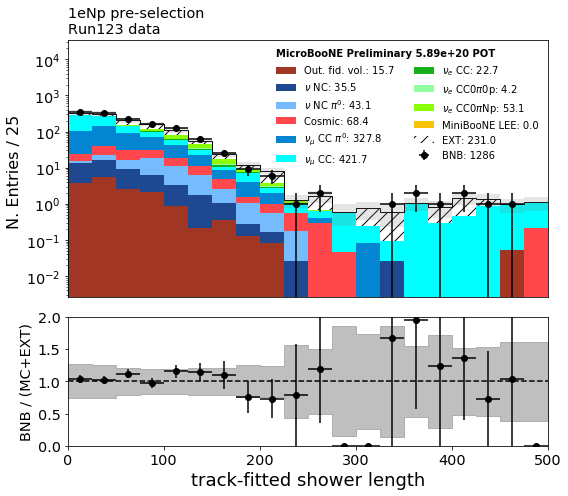
\includegraphics[width=1.00\textwidth]{Sidebands/Figures/CutUpdates/1eNp_HE_shr_trk_len.png}
    %\caption{\npsel Preselection}
    \end{subfigure}
    \caption{\label{fig:sb:cuts:shrlen} Reconstructed track-fitted shower length for \npsel pre-selection data from the high-energy sideband.}
    \end{center}
\end{figure}

\subsubsection{Number of Collection-plane Hits in Missed Shower}
\label{sec:sideband:newcuts:nhits}
Investigations of the Run1 open data as well as the \npsel high energy sideband showed that a few good candidate \nuecc events were failing the selection due to a cut on the number of collection-plane hits in clusters that are not matched in 3D (possibly due to showers not fully reconstructed). Events failing this cut included those in Fig.~\ref{fig:1eNp:box:evd}, due to the incomplete reconstruction of part of the electron shower in one case, and of the proton reinteraction in the other case.

We do not find this variable to be mismodeled based on high statistics sidebands (see Fig.~\ref{fig:sb:cut:secondshowerYnhit}). However, given that it has no impact on the analysis sensitivity, in order to gain signal efficiency we decided to remove (loosen) the requirements on this variable from the \npsel loose and tight box cuts (\zpsel BDT selection). 

Note that this variable is still used as part of the unmatched shower rejection cuts, where it is used more safely in conjunction with other variables. Similarly the variable is also kept among the BDT inputs. More details on the change to the Np selection can be found in DocDB 30202 and for the 0p selection in DocDB 30280.

\begin{figure}[H]
    \begin{center}
    \begin{subfigure}{0.45\textwidth}
    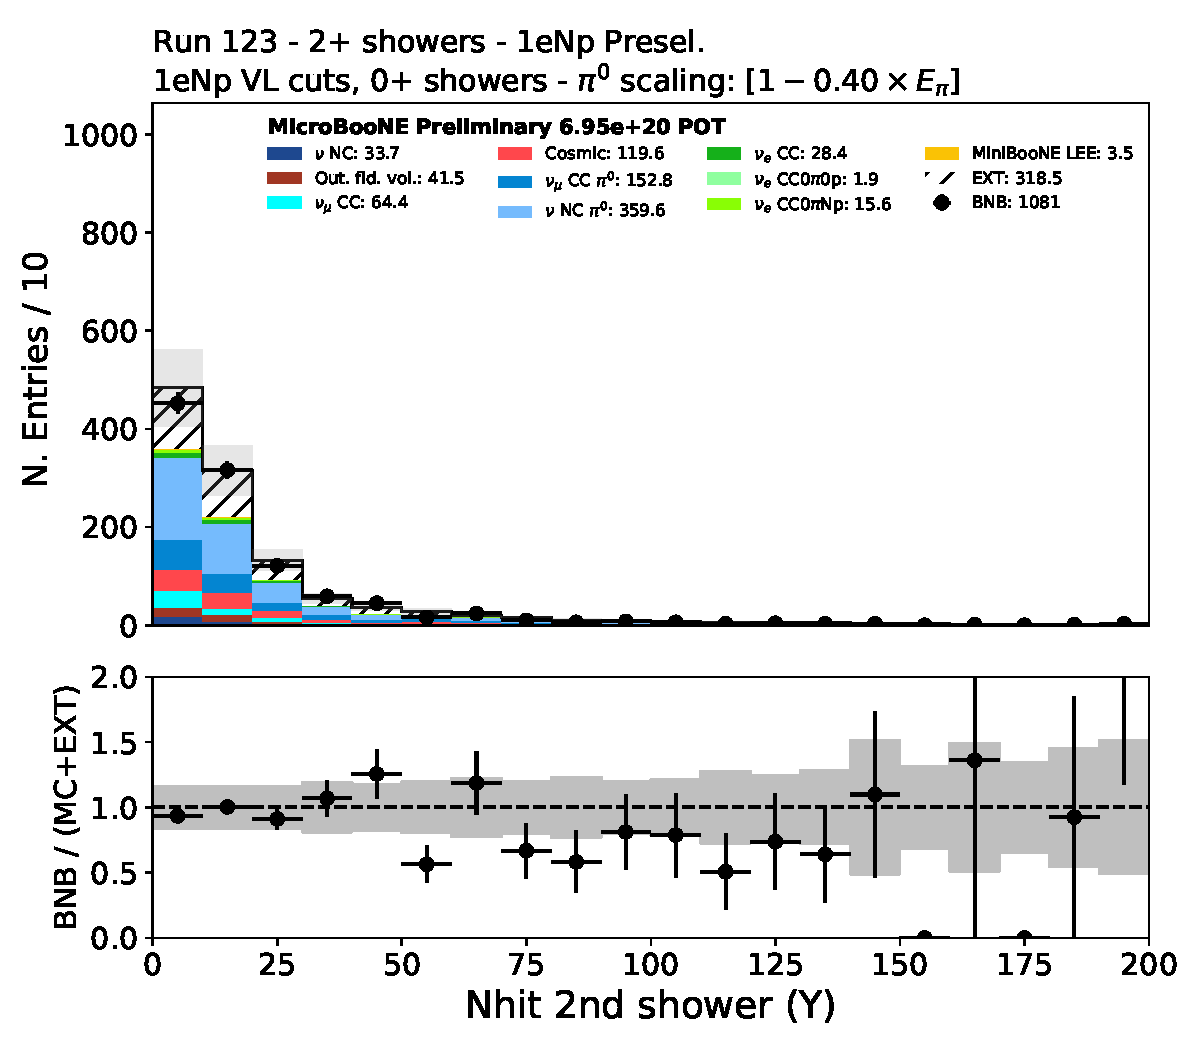
\includegraphics[width=1.00\textwidth]{Sidebands/Figures/CutUpdates/1eNp_2Shr_VL_secondshower_Y_nhit.pdf}
    %\caption{}
    \end{subfigure}
    \begin{subfigure}{0.45\textwidth}
    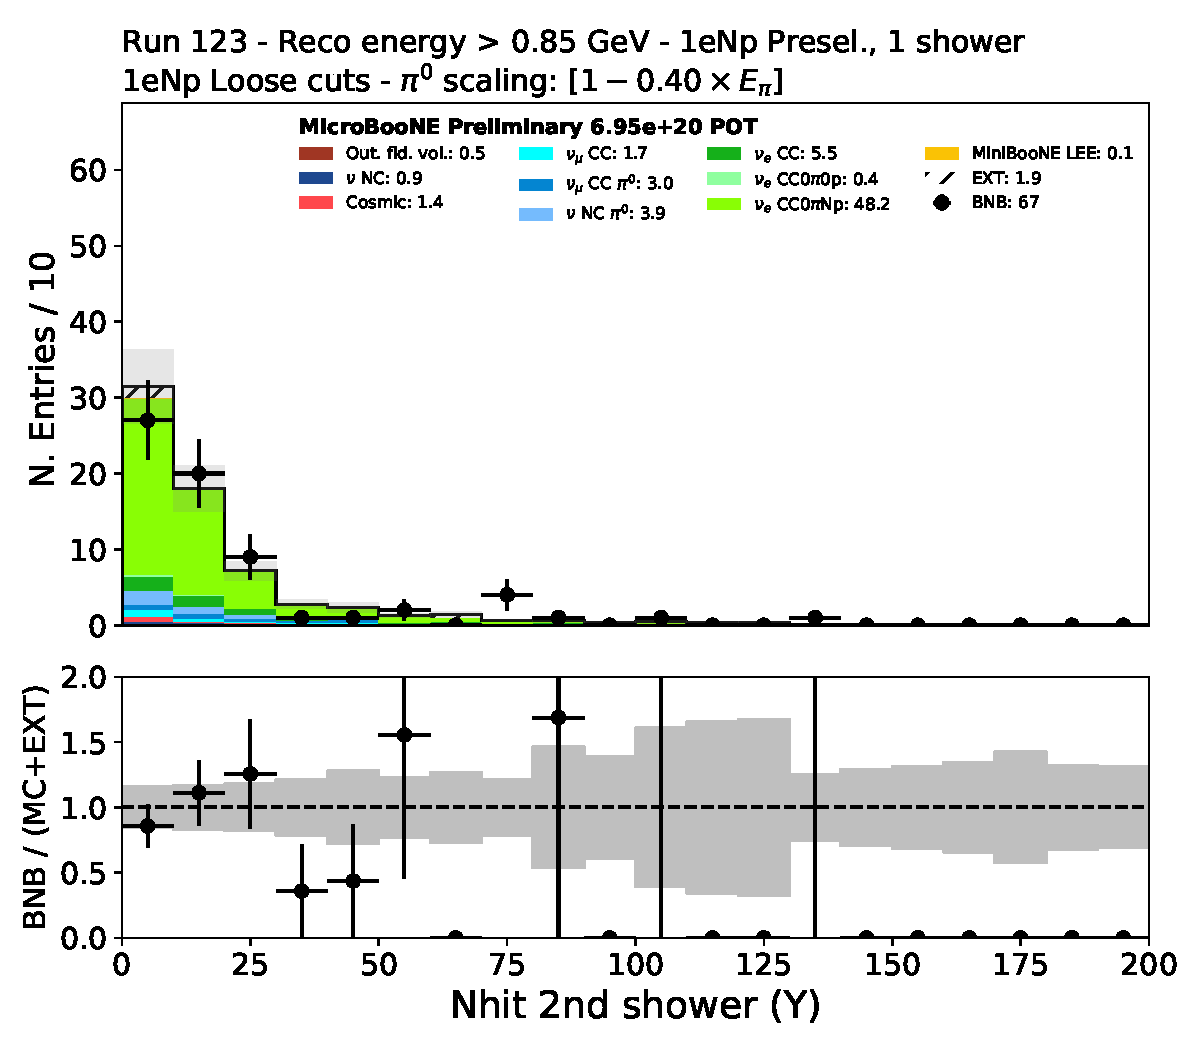
\includegraphics[width=1.00\textwidth]{Sidebands/Figures/CutUpdates/1eNp_HE_L_secondshower_Y_nhit.pdf}
    %\caption{}
    \end{subfigure}
    \caption{\label{fig:sb:cut:secondshowerYnhit} Number of collection-plane hits in clusters that are not matched in 3D with Run1+2 data in the \npsel 2+shower sideband after VeryLoose cuts (left) and in the \npsel high energy sideband after Loose cuts (right).}
    \end{center}
\end{figure}

\subsubsection{Shower Endpoint Cut}
\label{sec:sideband:newcuts:shrendpoint}
There is now 60\% more EXT data available to estimate the cosmic background in the electron neutrino selections.  These additional statistics available for the background estimation motivated adding an additional cut to remove cosmics in the 1e0p selection.  

Showers identified in the electron neutrino selections are also reconstructed as tracks.  Fig.~\ref{fig:1e0p:run123:shrstartend} shows the start and end point in the y direction at pre-selection in the open data. The peaked distribution makes it possible to add a cut in the y direction which suppresses the remaining EXT with minimal impact on the electron neutrino and LEE signals. Shower start points in the y direction are required to be within -100 cm and 80 cm, and end points in the y direction are required to be within -100 and 100. These cuts are fully documented in DocDBs 30130, 30277, and 31898.

\begin{figure}[H] 
\begin{center}
    \begin{subfigure}[b]{0.45\textwidth}
    \centering
    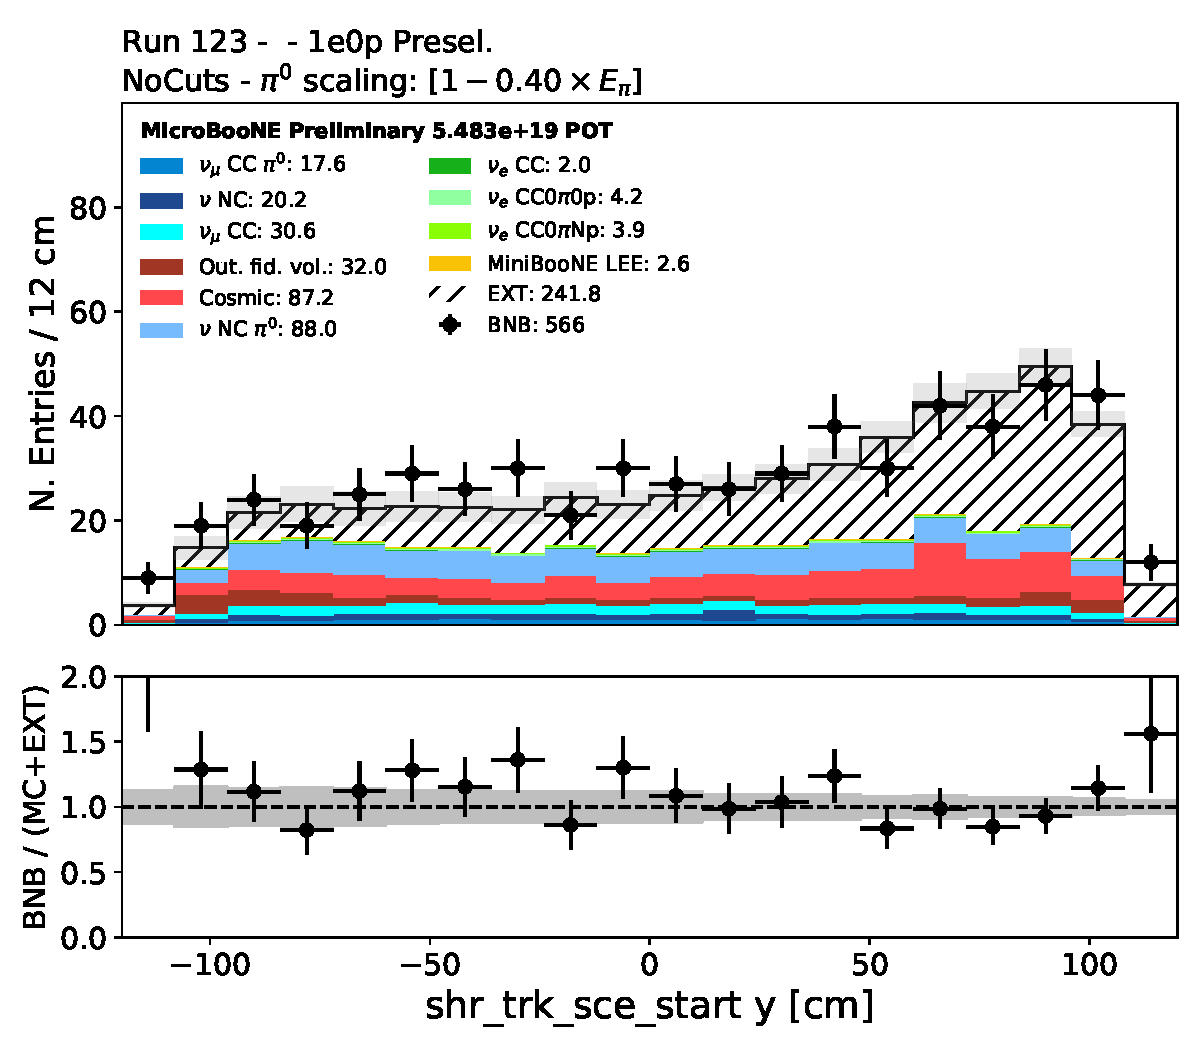
\includegraphics[width=1.00\textwidth]{1e0p/dataMCRun123/shr_trk_sce_start_y.pdf}
    \caption{\label{fig:1e0p:dataMCRun1:shr_start_y} shr\_trk\_sce\_start\_y }
    \end{subfigure}
    \begin{subfigure}[b]{0.45\textwidth}
    \centering
    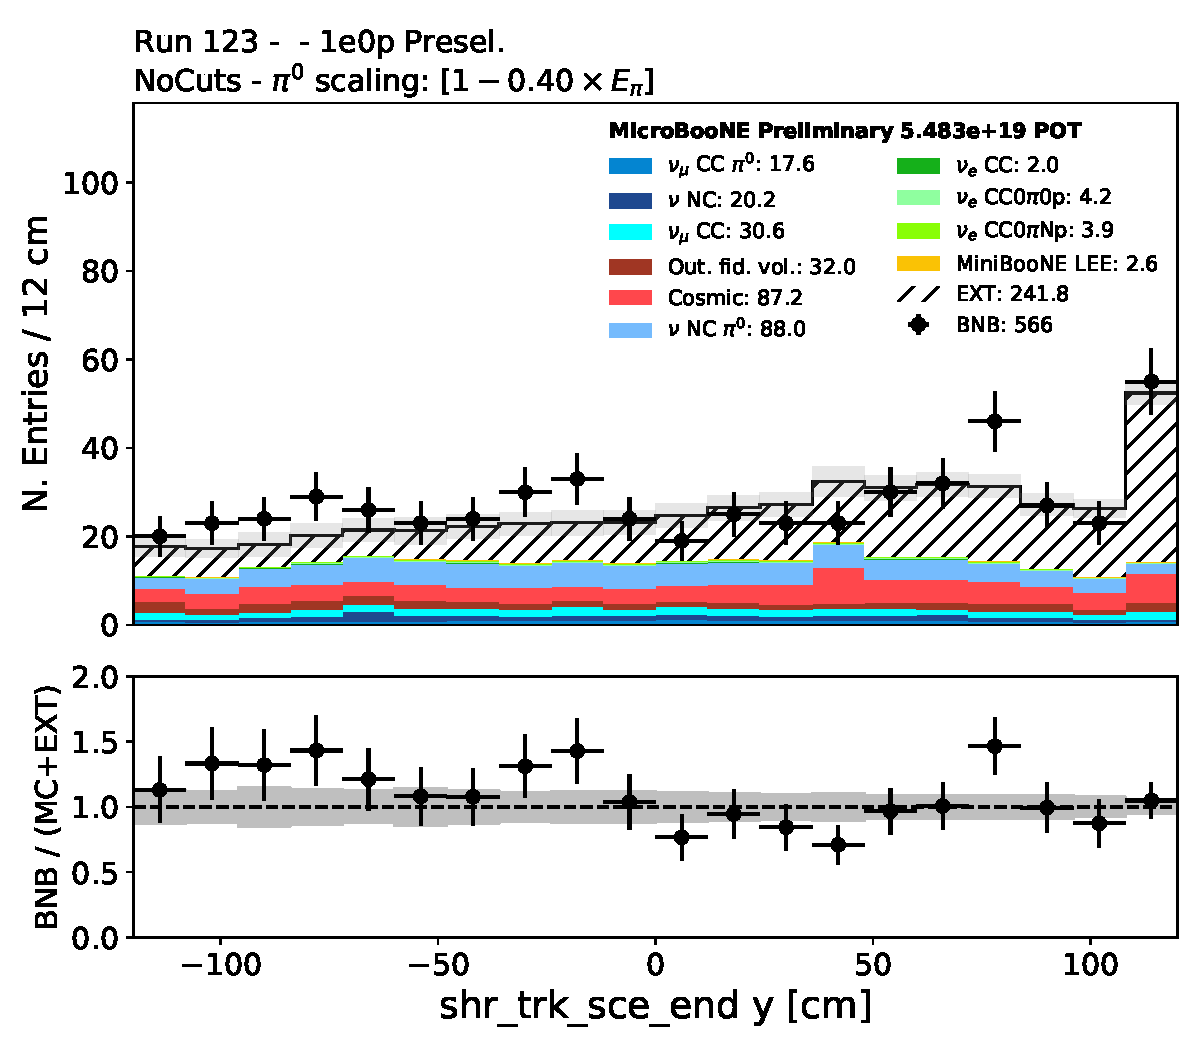
\includegraphics[width=1.00\textwidth]{1e0p/dataMCRun123/shr_trk_sce_end_y.pdf}
    \caption{\label{fig:1e0p:dataMCRun1:shr_end_y} shr\_trk\_sce\_end\_y }
    \end{subfigure}
\caption{\label{fig:1e0p:run123:shrstartend}Data-MC comparison in the open data after the \zpsel preselection.}
\end{center}
\end{figure}

\subsubsection{Exiting Track Cut}
\label{sec:sideband:newcuts:exitingtrack}
In the 1e0p high energy sideband it was observed that there were events with exiting tracks passing the selection. These events pass the 0p selection because previously the only cut on the number of tracks was to require no contained tracks, which allowed events with exiting tracks to make it into the selection. 

One of the events with an exiting track is a cosmic event which is reconstructed as a back to back shower and track. These events can be removed from the 1e0p selection by requiring either 0 tracks total, or 1 track, when the exiting track is back to back with the shower. 

The number of total tracks in events passing the 0p pre-selection is shown in Fig.~\ref{fig:1e0p:dataMCRun1:n_tk_tot}. For events that have more than one track the angle between the shower and track is shown in Fig.~\ref{fig:1e0p:dataMCRun1:shtkang}.  EXT events pile up below -0.9 in this distribution, so can be safely removed without impacting the signal.  

To summarize, events are required to have either zero total tracks, or the cosine of the angle of the exiting track must be greater than -0.9 relative to the shower direction. 

This cut is fully documented in DocDB 31691.

\begin{figure}[H] 
\begin{center}
    \begin{subfigure}[b]{0.45\textwidth}
    \centering
    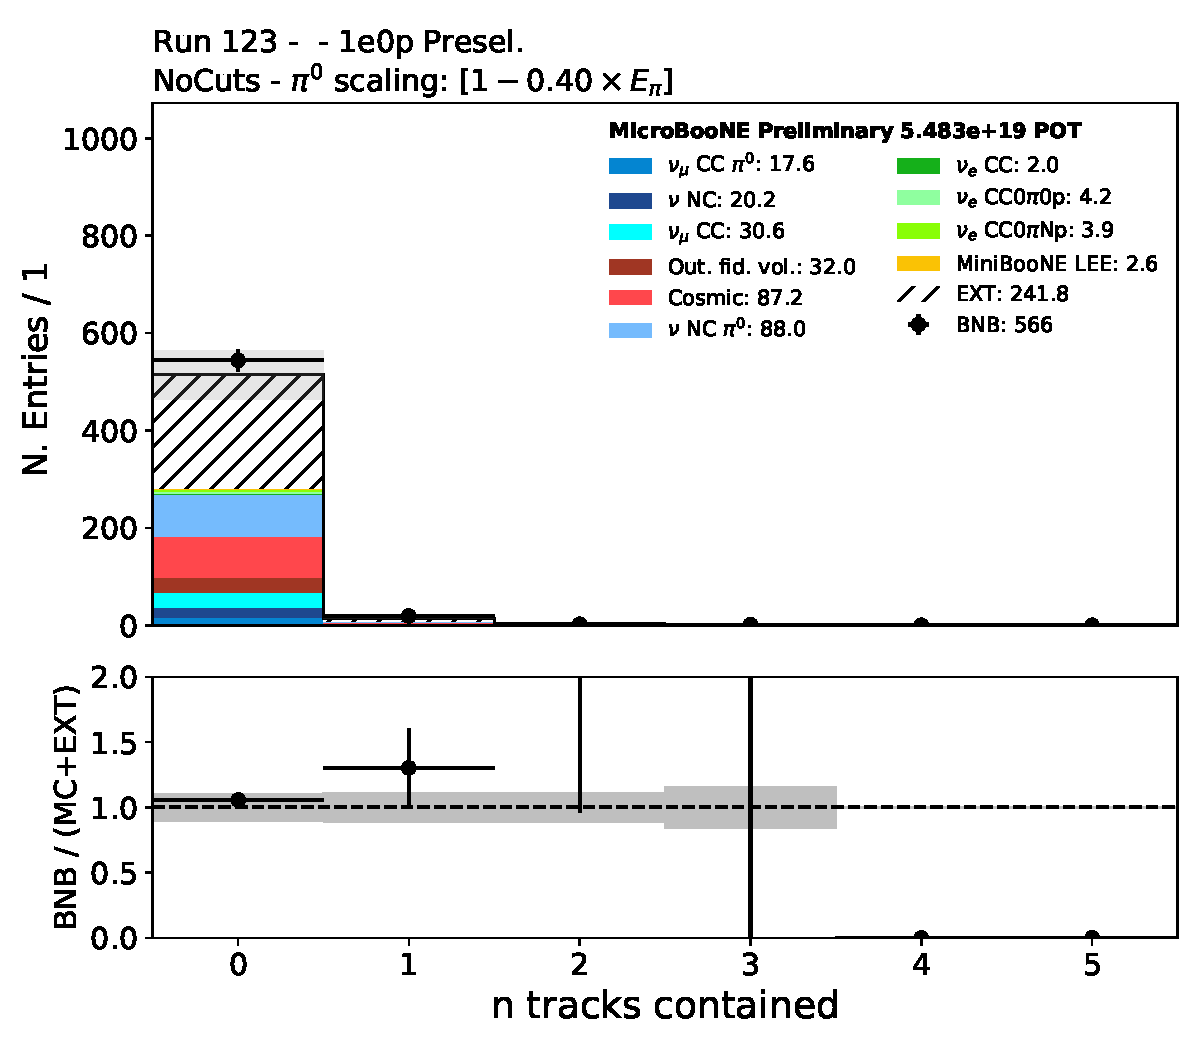
\includegraphics[width=1.00\textwidth]{1e0p/dataMCRun123/n_tracks_tot.pdf}
    \caption{\label{fig:1e0p:dataMCRun1:n_tk_tot} n tracks tot }
    \end{subfigure}
    \begin{subfigure}[b]{0.45\textwidth}
    \centering
    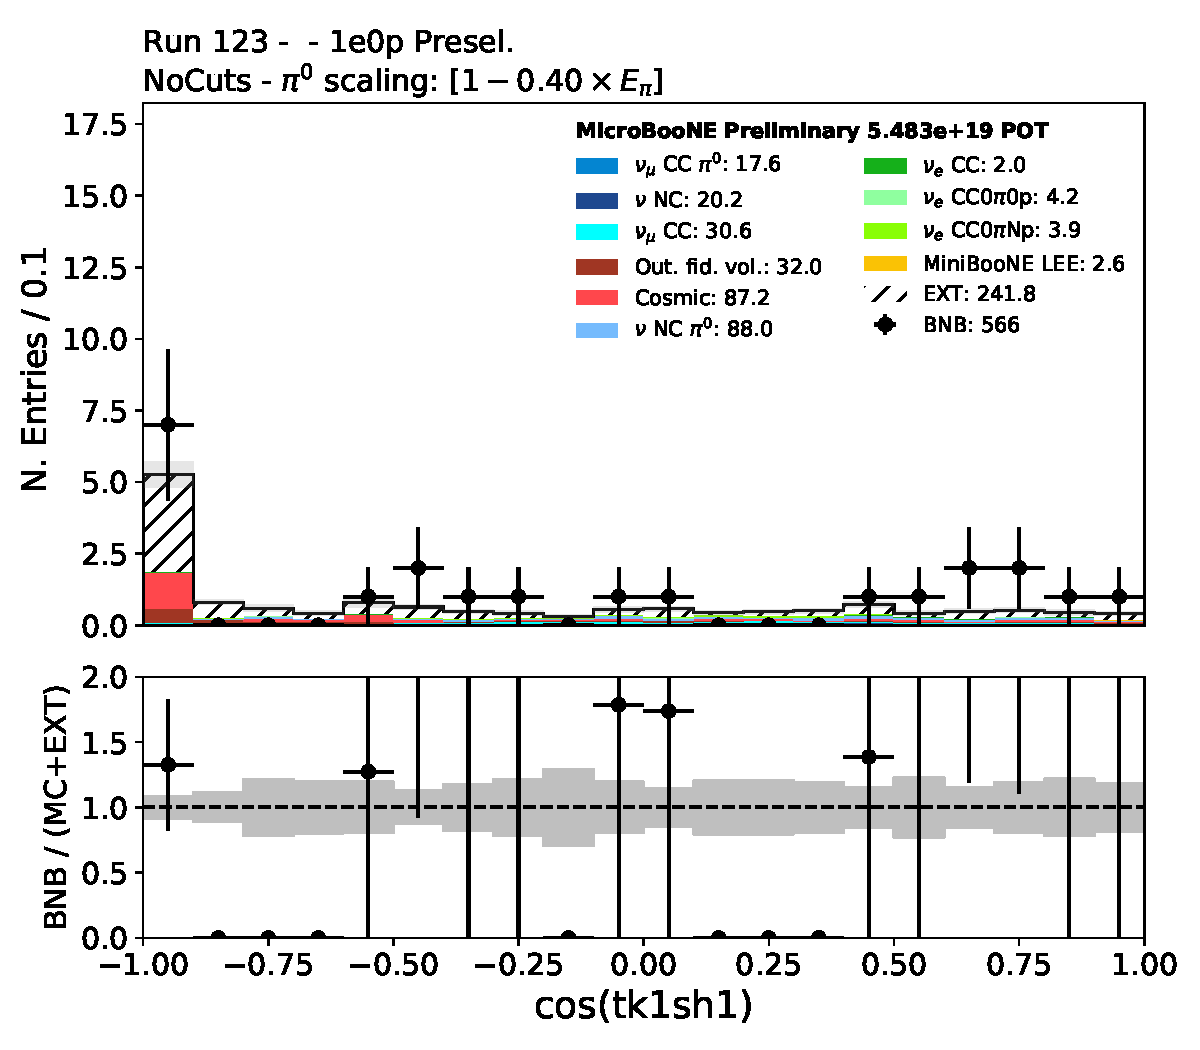
\includegraphics[width=1.00\textwidth]{1e0p/dataMCRun123/tk1sh1_angle_alltk.pdf}
    \caption{\label{fig:1e0p:dataMCRun1:shtkang} tk1 sh1 angle alltk }
    \end{subfigure}
\caption{\label{fig:1e0p:dataMCRun1:exitingtrack_opendata}Data-MC comparison in the open data after the \zpsel preselection.}
\end{center}
\end{figure}

\begin{comment}
\subsubsection{Second Shower Number of Hits Cut}
It was observed in the high energy sideband that the cut on the number of hits in the second shower on the y plane removed signal events, and therefore was not beneficial for the overall Np and 0p selections.

In the Np selection the cut is removed entirely, and in the 0p selection the cut is relaxed from requiring fewer than 20 hits to fewer than 50 hits.  The change to the Np selection is documented in DocDB 30202 and for the 0p selection in DocDB 30280.

\begin{figure}[H] 
\begin{center}
    \begin{subfigure}[b]{0.45\textwidth}
    \centering
    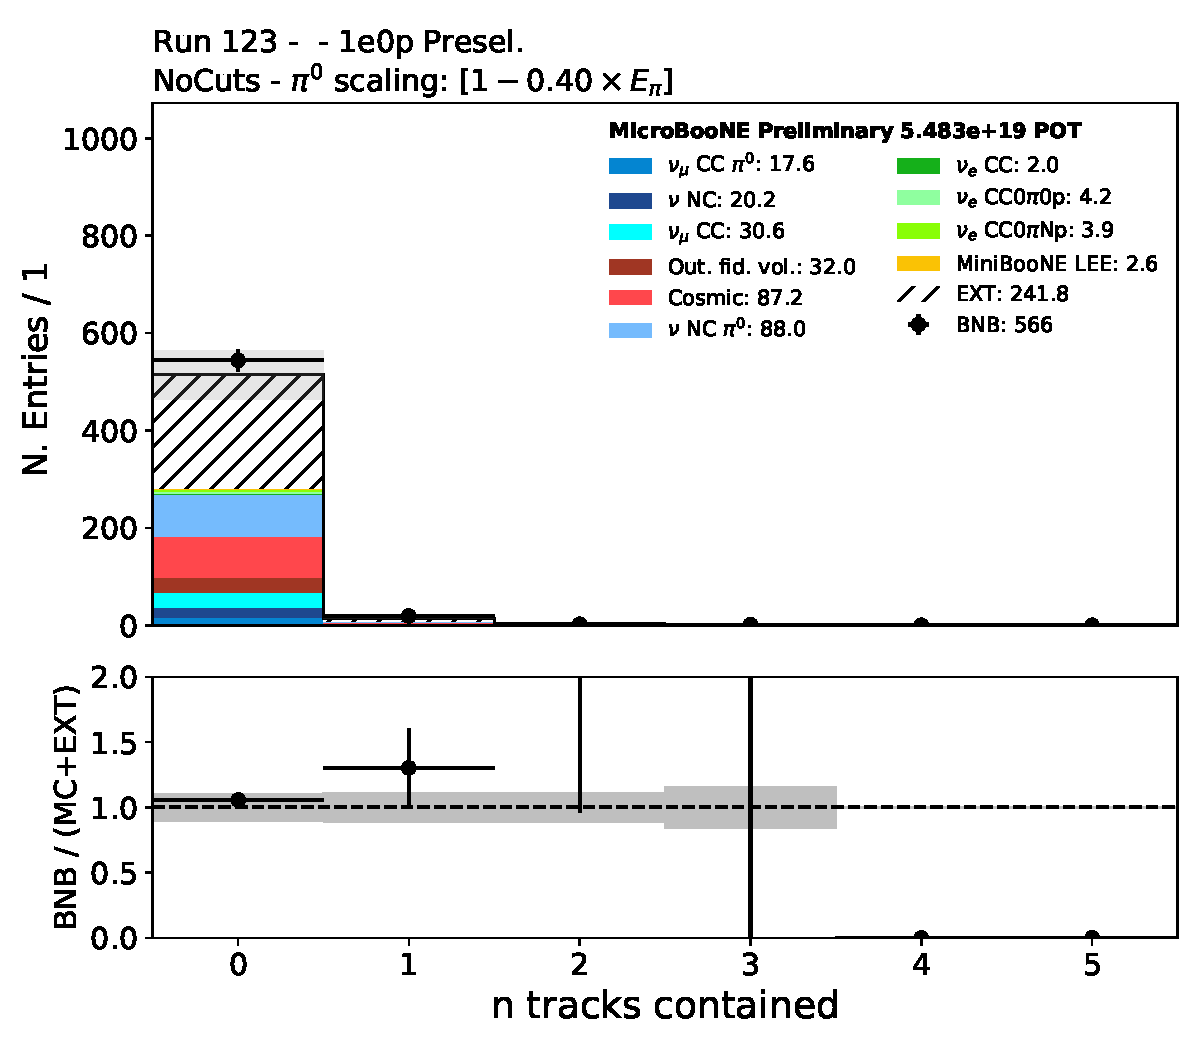
\includegraphics[width=1.00\textwidth]{1e0p/dataMCRun123/n_tracks_tot.pdf}
    \caption{\label{fig:1e0p:dataMCRun1:n_tk_tot} n tracks tot }
    \end{subfigure}
    \begin{subfigure}[b]{0.45\textwidth}
    \centering
    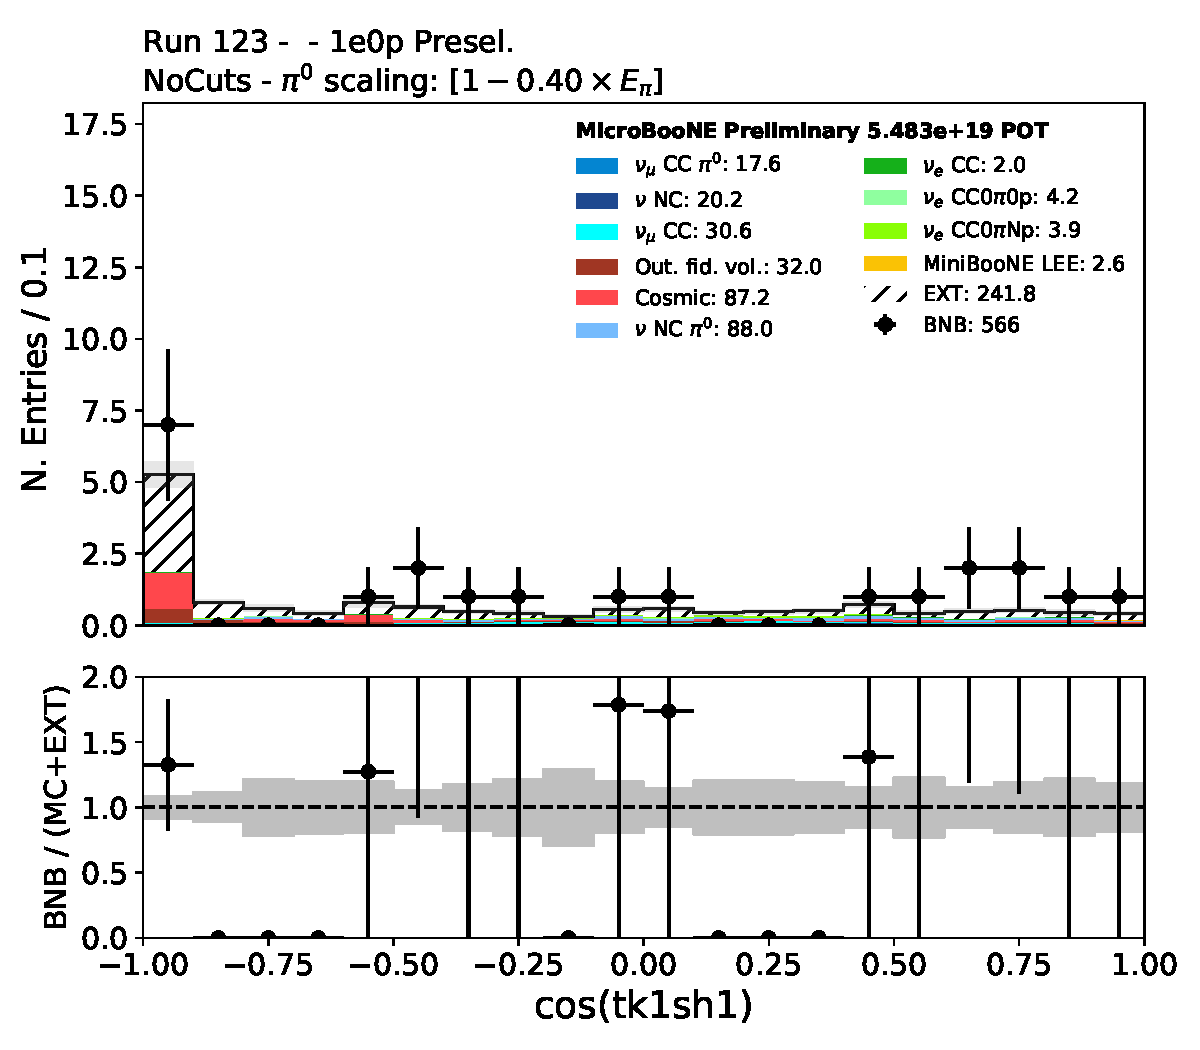
\includegraphics[width=1.00\textwidth]{1e0p/dataMCRun123/tk1sh1_angle_alltk.pdf}
    \caption{\label{fig:1e0p:dataMCRun1:shtkang} tk1 sh1 angle alltk }
    \end{subfigure}
\caption{\label{fig:1e0p:dataMCRun1:exitingtrack_opendata}Data-MC comparison in the open data after the \zpsel preselection.}
\end{center}
\end{figure}
\end{comment}

\subsection{\npsel Sidebands}
\label{sec:sideband:1eNp}
\subsubsection{Two+ Shower Sideband}
\label{sec:sideband:1eNp:2pshr}
The sideband with at least two reconstructed showers provides an extremely valuable sample, where the analysis can be validated inclusively in terms of neutrino energy and BDT response. In particular, given that this sideband is enriched in $\pi^0$ contribution, it allows for a detailed study of the $\pi^0$ modeling across all analysis selection stages; the only difference with respect to the nominal selections is that the requirement of only one contained shower has been replaced with the requirement of two or more showers.

Fig.~\ref{fig:sb:1eNp:twopshr:recoe} shows the reconstructed neutrino energy distributions at different selection stages: \npsel preselection, very loose cuts, and loose cuts; as previously discussed in sec.~\ref{sec:pi0tune}, an energy-dependent scaling is applied to the \pizero contribution. The agreement is very good at pre-selection stage, while it shows a mild deficit (well within systematic uncertainties) in the other stages.

\begin{figure}[H]
    \begin{center}
    \begin{subfigure}{0.32\textwidth}
    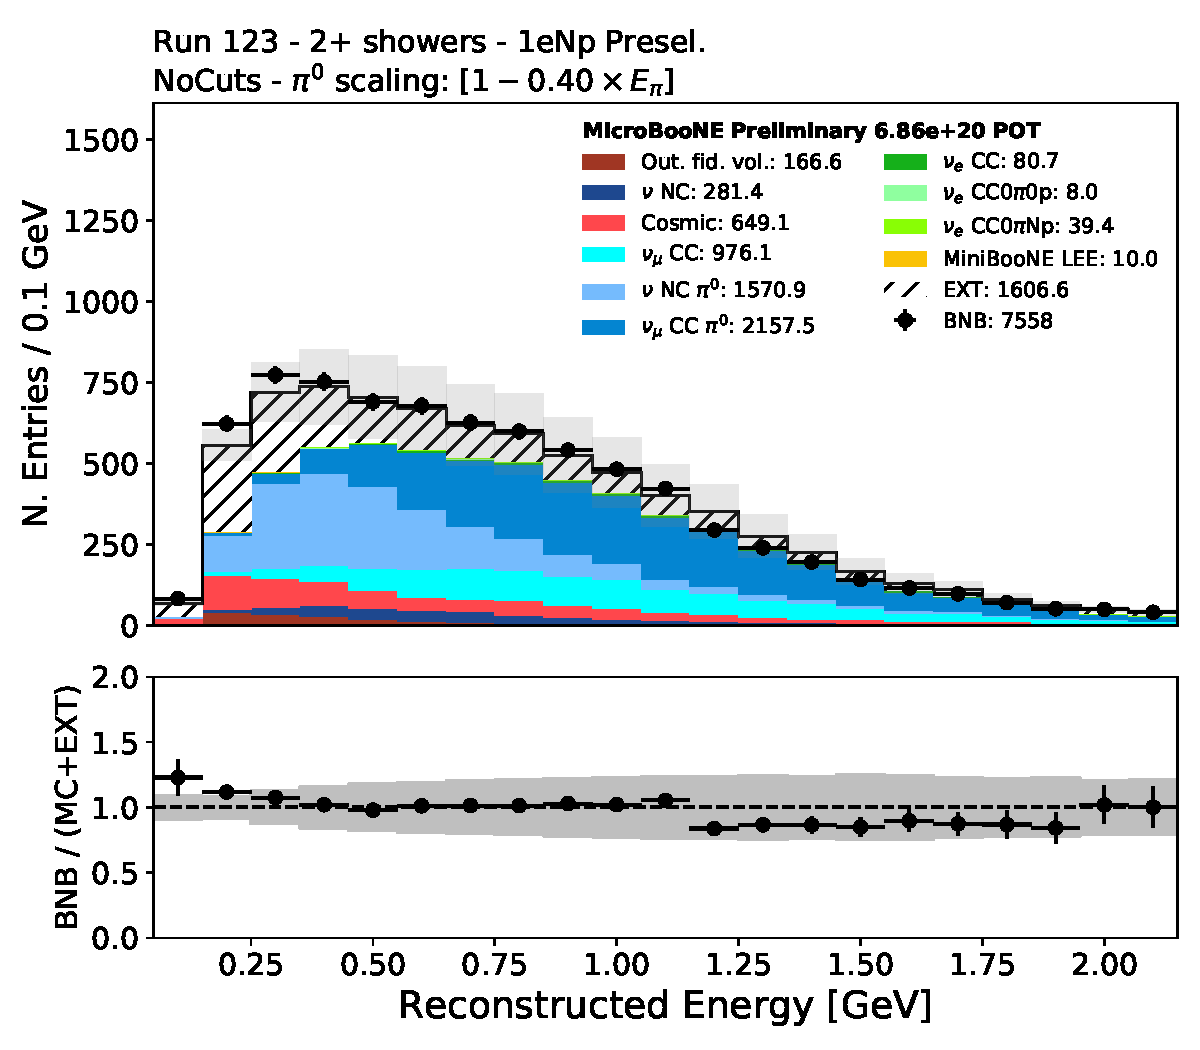
\includegraphics[width=1.00\textwidth]{Sidebands/Figures/1eNp/TwoShower/TwoPShr_NP_None_pi0e040/reco_e.pdf}
    \caption{\npsel Preselection}
    \end{subfigure}
    \begin{subfigure}{0.32\textwidth}
    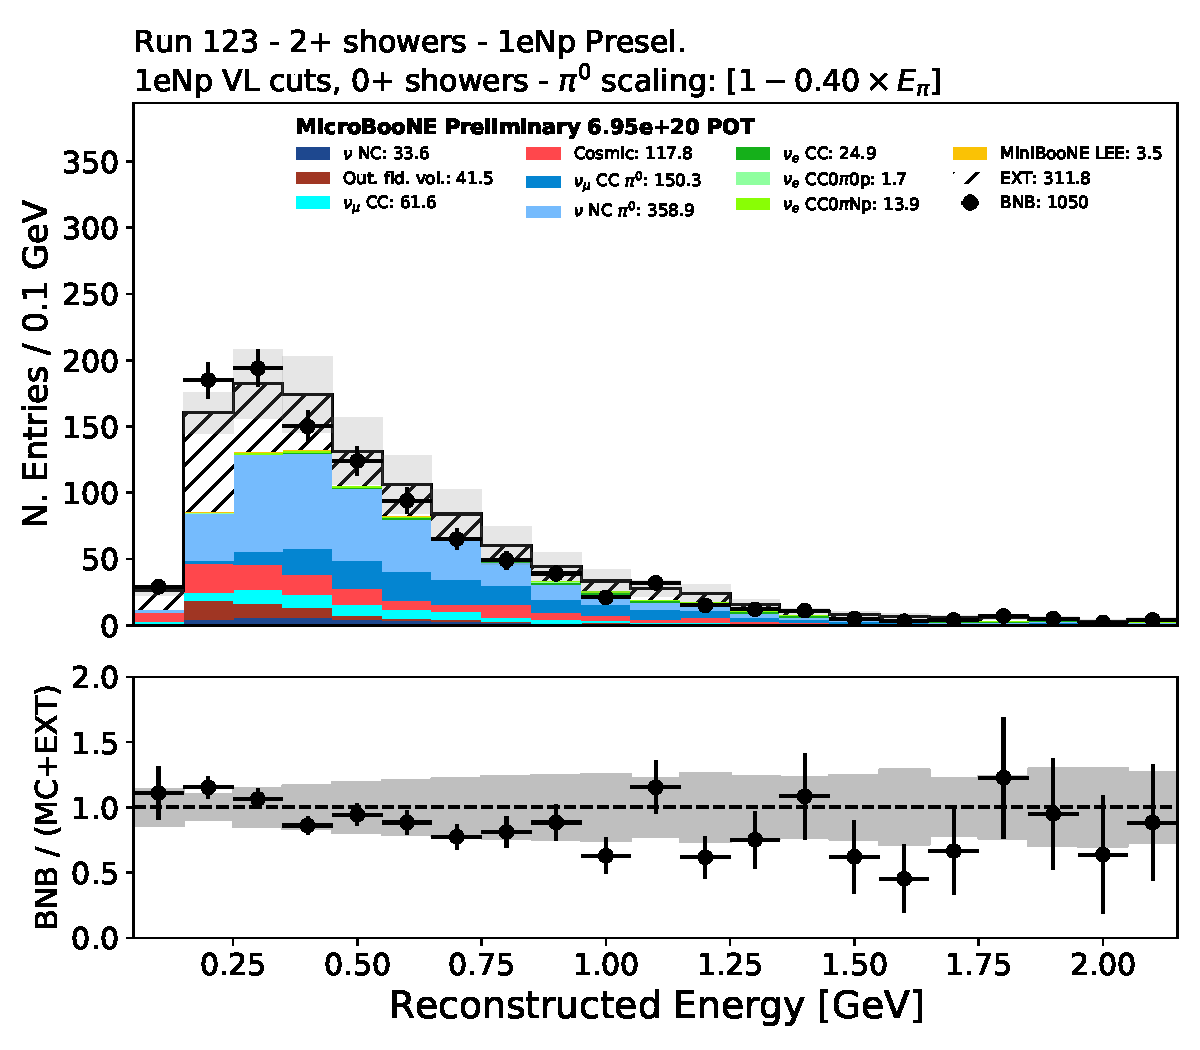
\includegraphics[width=1.00\textwidth]{Sidebands/Figures/1eNp/TwoShower/TwoPShr_NP_NPVLAllShr_pi0e040/reco_e.pdf}
    \caption{\npsel VeryLoose cuts}
    \end{subfigure} 
    \begin{subfigure}{0.32\textwidth}
    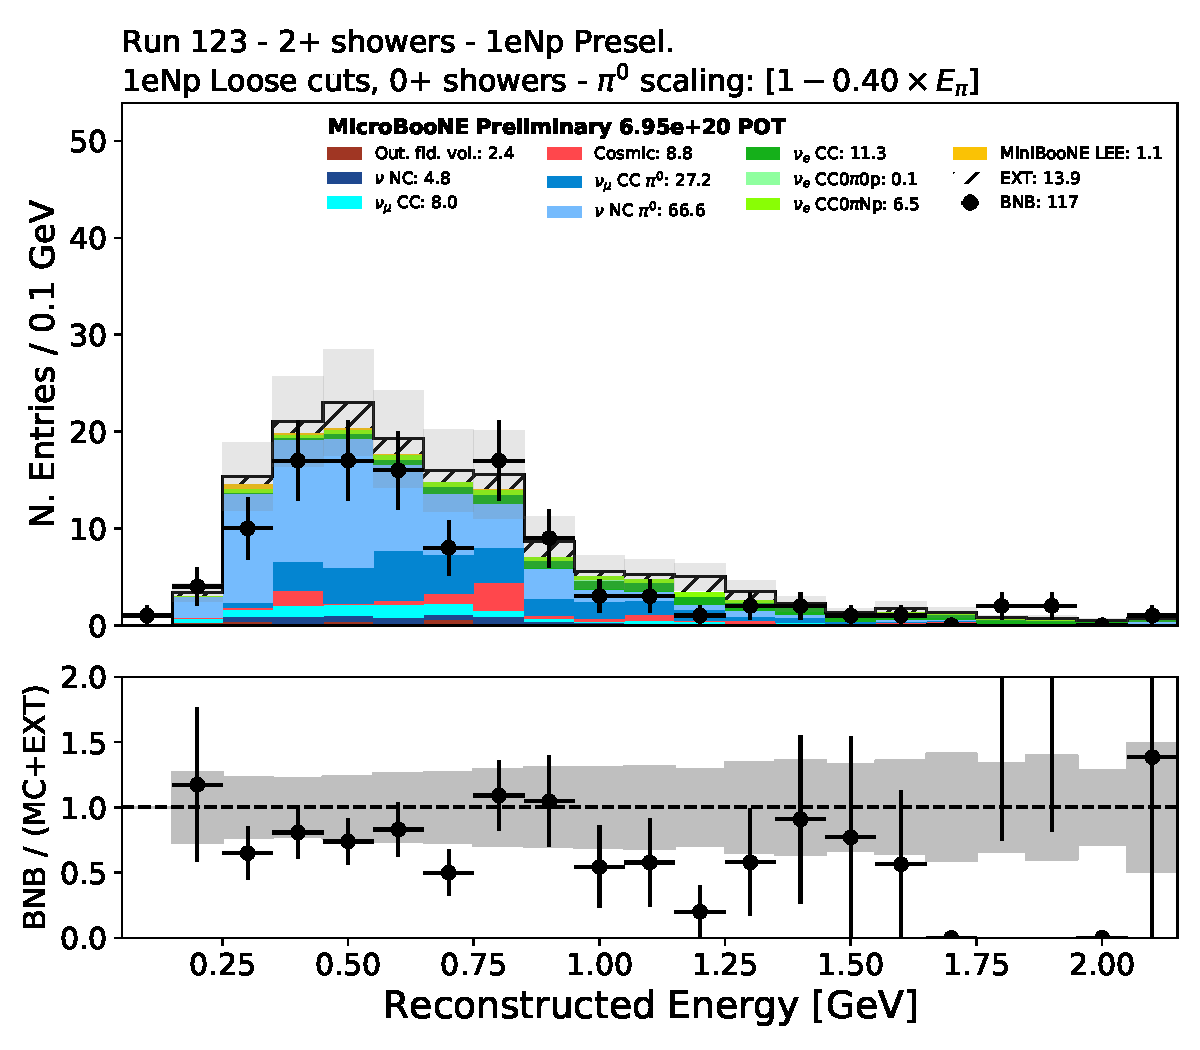
\includegraphics[width=1.00\textwidth]{Sidebands/Figures/1eNp/TwoShower/TwoPShr_NP_NPLAllShr_pi0e040/reco_e.pdf}
    \caption{\npsel Loose cuts}
    \end{subfigure}
    \caption{\label{fig:sb:1eNp:twopshr:recoe} Reconstructed neutrino energy in the 2+ shower sideband, at different stages of the \npsel selection.}
    \end{center}
\end{figure}

As shown in Appendix~\ref{app:sideband:1eNptwoplusshower}, distributions of the BDT input variables at Loose selection stage shows reasonable agreement. However, some tension is present in a few variables, especially in signal-like bins, which then translates into a deficit in the highest BDT score bins (Fig.~\ref{fig:sb:1eNp:twopshr:loose:dedxbdt}). After including systematic uncertainties (all except detector), the probability of the BDT distribution is at about 1-sigma level.

\begin{figure}[H]
    \begin{center}
    \begin{subfigure}{0.4\textwidth}
    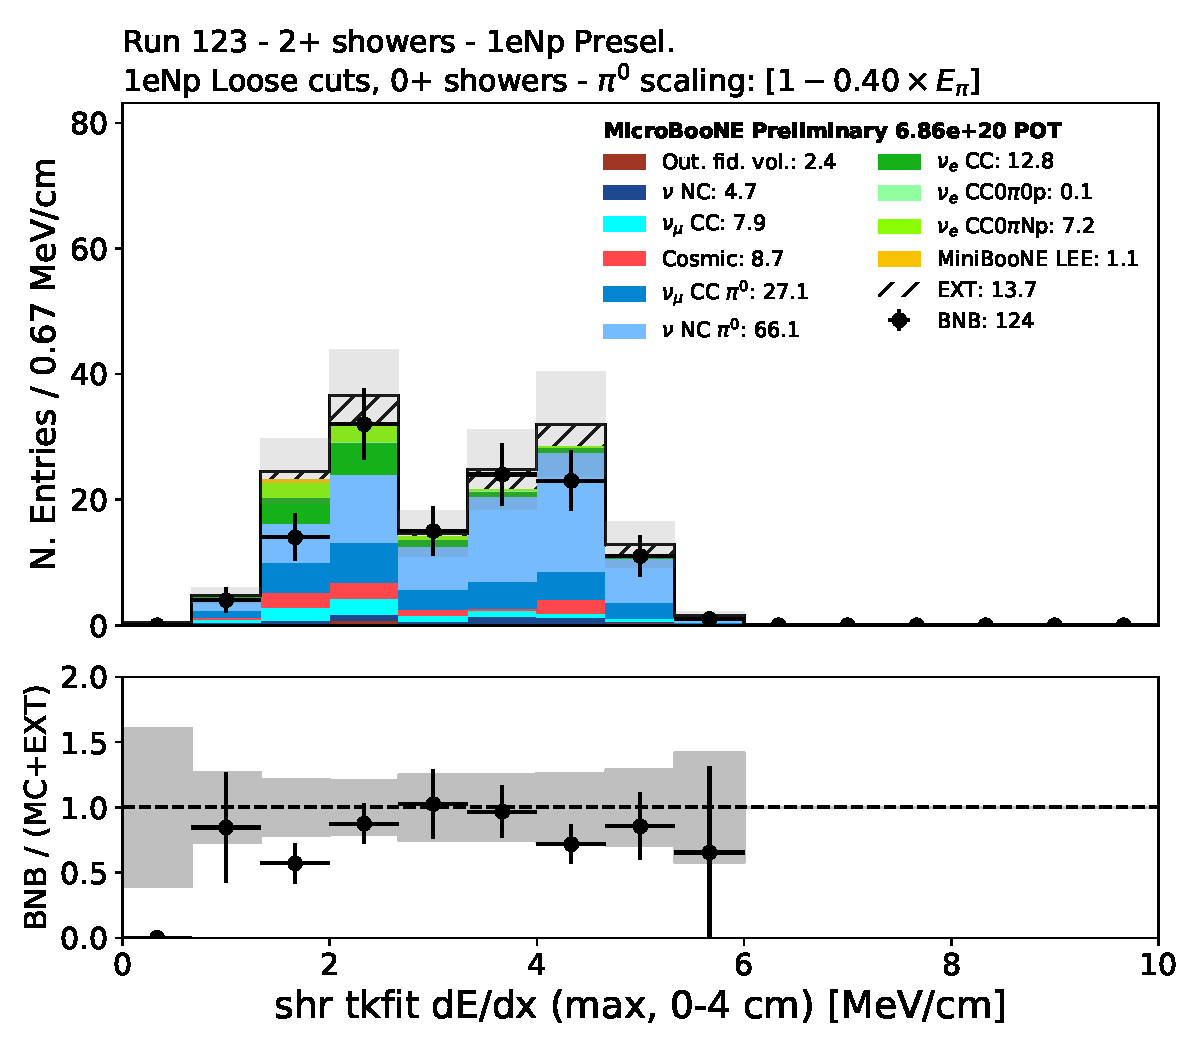
\includegraphics[width=1.00\textwidth]{Sidebands/Figures/1eNp/TwoShower/TwoPShr_NP_NPLAllShr_pi0e040/shr_tkfit_dedx_max.pdf}
    \end{subfigure}
    \begin{subfigure}{0.4\textwidth}
    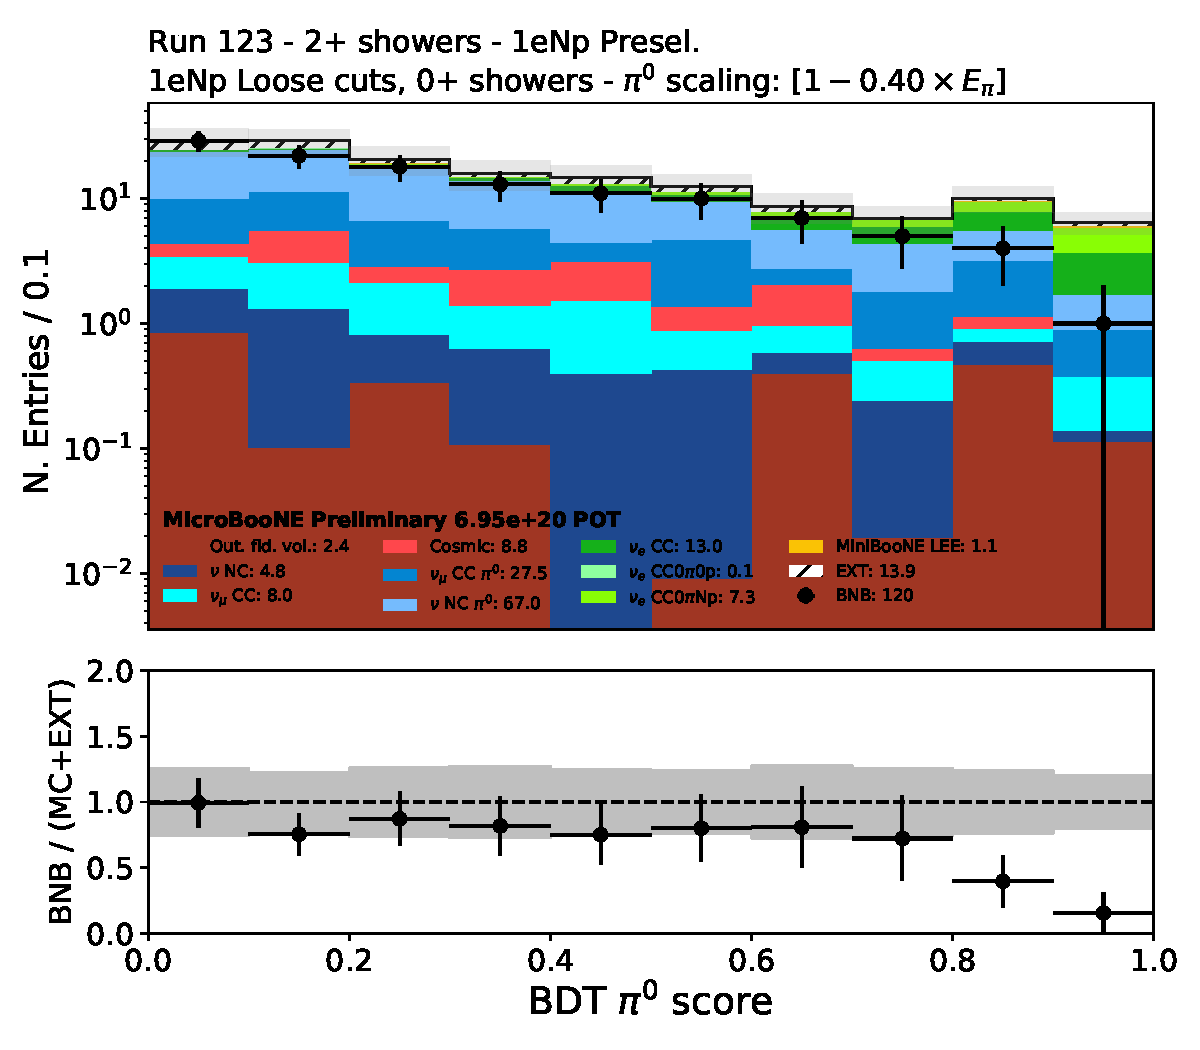
\includegraphics[width=1.00\textwidth]{Sidebands/Figures/1eNp/TwoShower/TwoPShr_NP_NPLAllShr_pi0e040/pi0_score_log.pdf}
    \end{subfigure}
    \caption{\label{fig:sb:1eNp:twopshr:loose:dedxbdt} Shower dEdx and BDT response in the 2+ shower sideband, at Loose stage of the \npsel selection.}
    \end{center}
\end{figure}

As a consequence of the deficit in the last bin of the BDT response, the BDT selection also shows a deficit (Fig.~\ref{fig:sb:1eNp:twopshr:bdt:recoe}). Once again, despite being statistically significant, the severity of the deficit is largely mitigated when systematic uncertainties are taken into account and varies between well within 1 sigma to a bit more than 1 sigma depending on whether correlations are taken into account or neglected, respectively. 

\begin{figure}[H]
    \begin{center}
    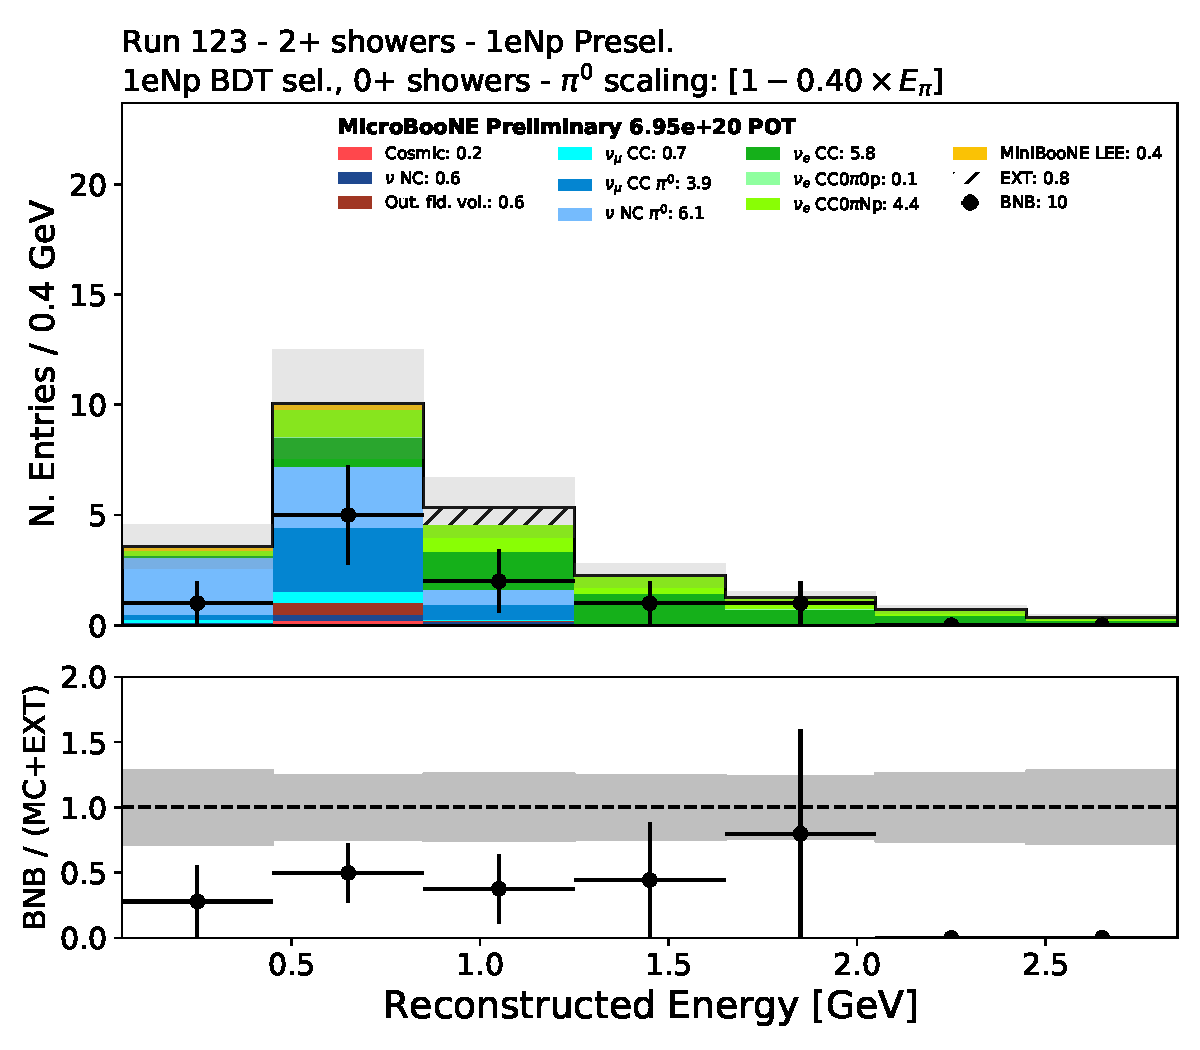
\includegraphics[width=0.4\textwidth]{Sidebands/Figures/1eNp/TwoShower/TwoPShr_NP_NPBDTAllShr_pi0e040/reco_e_coarse.pdf}
    \caption{\label{fig:sb:1eNp:twopshr:bdt:recoe} Reconstructed neutrino energy in the 2+ shower sideband, at BDT stage of the \npsel selection.}
    \end{center}
\end{figure}

We have carried out additional studies to understand more the deficit in this sideband. First, we looked at the event displays for the events passing the BDT selection (see DocDB 31760) and they seem to indicate that the observed number of \npsel and NC\pizero events is consistent with the expectations; the signal and the main background for the analysis thus behave as expected. Then we also looked at the Tight box cut selection, which is an alternative selection with comparable efficiency and purity with respect to the BDT (see Appendix~\ref{app:nueslections:1eNp}); in this selection, while we observe an excellent data-MC agreement in terms of reconstructed neutrino energy, we still see a deficit in signal-like bins for some variables that is qualitatively consistent with the result of the BDT selection (Fig.~\ref{fig:sb:1eNp:twopshr:tight}).

\begin{figure}[H]
    \begin{center}
    \begin{subfigure}{0.4\textwidth}
    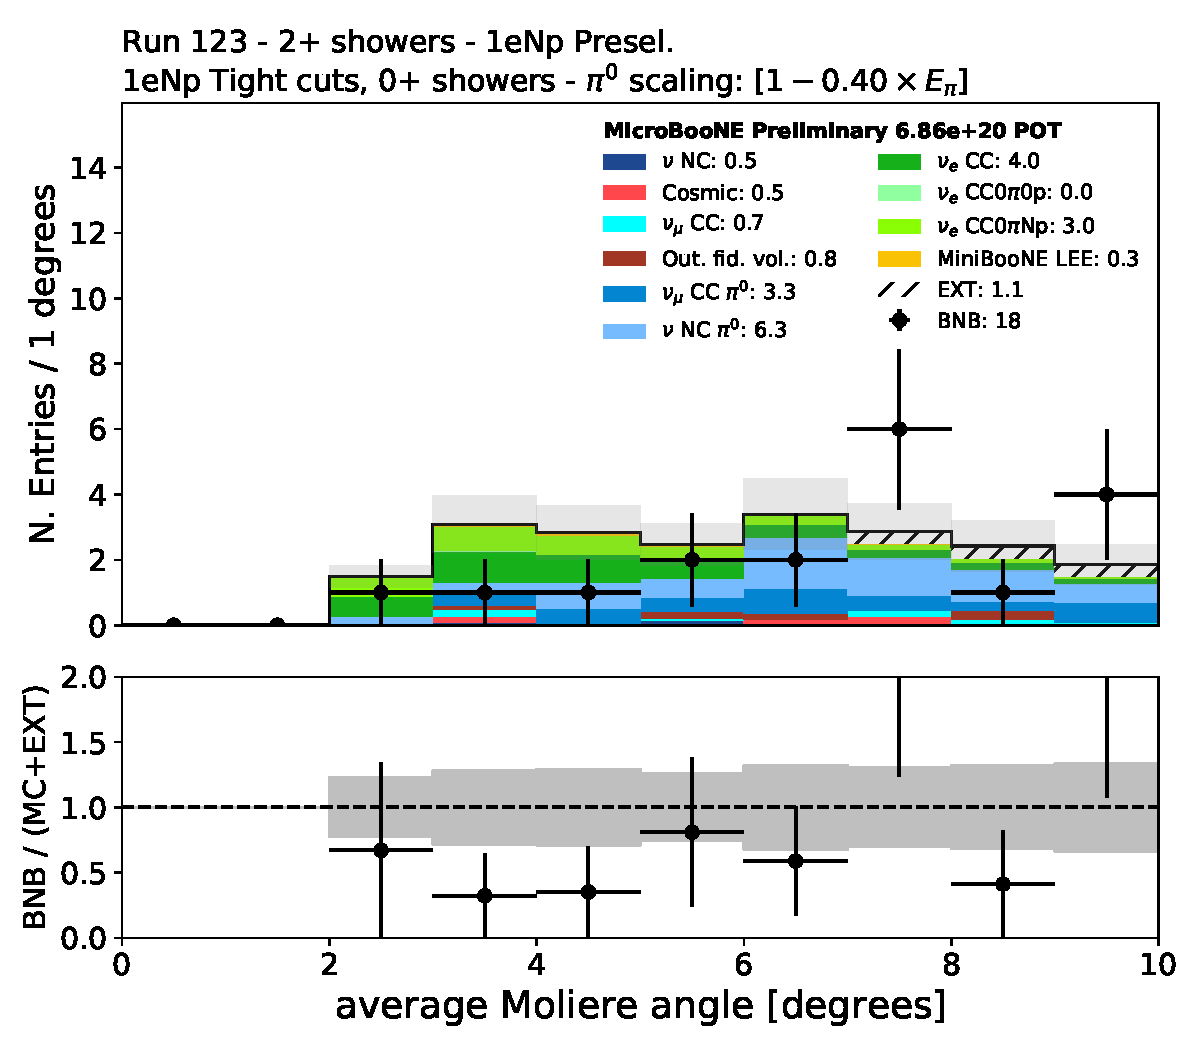
\includegraphics[width=1.00\textwidth]{Sidebands/Figures/1eNp/TwoShower/TwoPShr_NP_NPTAllShr_pi0e040/shrmoliereavg_zoomed.pdf}
    \end{subfigure}
    \begin{subfigure}{0.4\textwidth}
    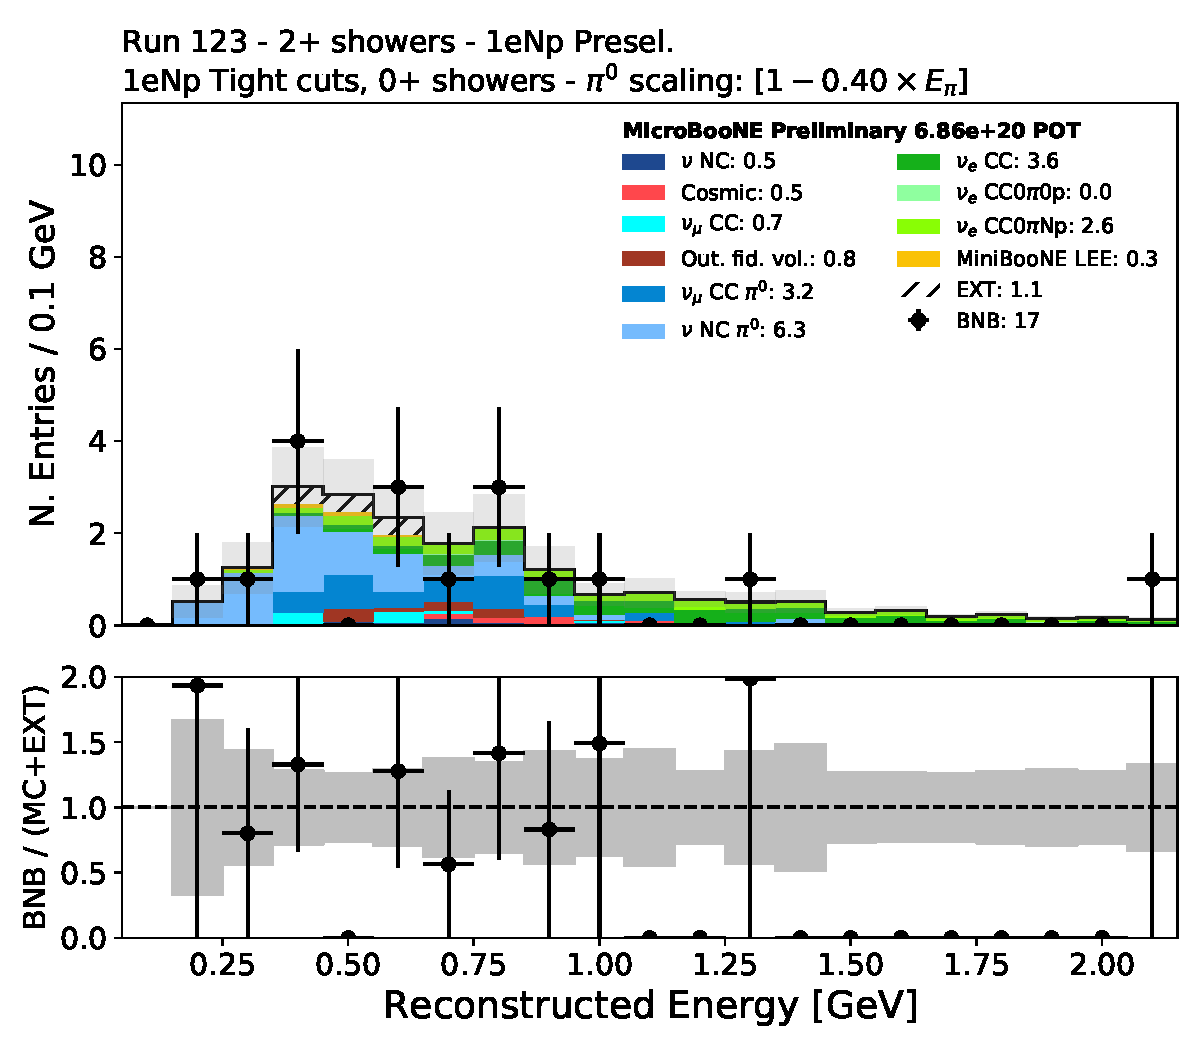
\includegraphics[width=1.00\textwidth]{Sidebands/Figures/1eNp/TwoShower/TwoPShr_NP_NPTAllShr_pi0e040/reco_e.pdf}
    \end{subfigure}
    \caption{\label{fig:sb:1eNp:twopshr:tight} Shower Moliere angle and reconstructed neutrino energy in the 2+ shower sideband, at Tight stage of the \npsel selection.}
    \end{center}
\end{figure}

In summary, the \npsel 2+ shower sideband validates the NC\pizero background of the analysis and, depending on the selection, it shows good agreement or a deficit covered by the systematic uncertainties included in the analysis. The observation of a deficit in events shown at BDT-selection stage (fig.~\ref{fig:sb:1eNp:twopshr:bdt:recoe}), concentrated in bins populated by \nue events (fig.~\ref{fig:sb:1eNp:twopshr:loose:dedxbdt}),raises question on the origin of this discrepancy. While no clear conclusion can be drawn, and the limited phase space selected with the full BDT selection may further compicate interpretations, it will be important to keep these observations in mind as the analysis progresses to the near-sideband data. This sideband provides a particularly valuable validation of input variables to the \nue selection in $\pi^0$ rich distributions, which, when plotted at pre-selection stage with high statistics (see appendix~\ref{app:sideband:1eNptwoplusshower}), show very good data/mc agreement.

\subsubsection{High Energy Sideband}
\label{sec:sideband:1eNp:he}
The high-energy sideband opens in an unbiased way all events with a reconstructed energy greater than 0.85 GeV. The final result of this sideband is in Figure~\ref{fig:HE_1eNp_reco_e}, which shows the reconstructed energy spectrum for \npsel after the BDT selection using the available 6.9e20 POT from Runs 1, 2, and 3.
\begin{figure}[H]
    \begin{center}
    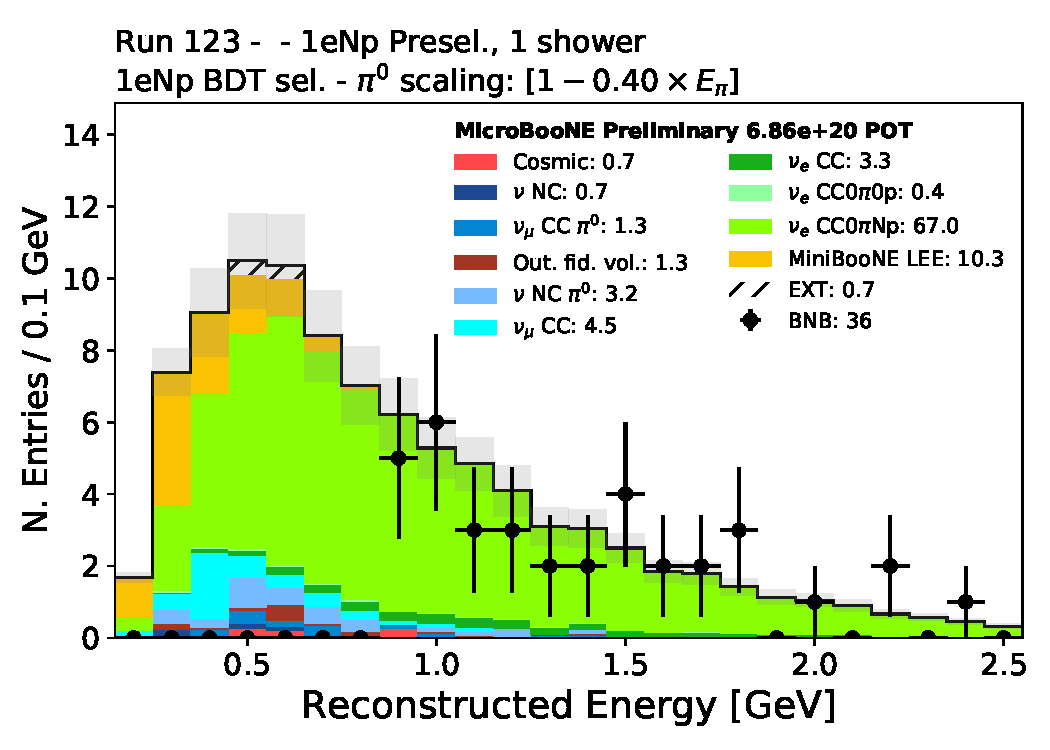
\includegraphics[width=0.5\textwidth]{Sidebands/Figures/1eNp/HighEnergy/reco_e.pdf}
    \caption{Reconstructed neutrino energy in the high energy sideband, after the final stage (BDT) of the \npsel selection. MC is plotted for all energies, and BNB data only for the energies at which it is open; above 0.85 GeV.}
    \label{fig:HE_1eNp_reco_e}
    \end{center}
\end{figure}

At different selection stages, different processes dominate the event sample: at pre-selection $\nu_\mu$ interactions (with and without \pizero) are the most abundant, while at VeryLoose and Loose selection stages, \nuecc interactions already dominate. In all cases we find good data-MC agreement (Fig.~\ref{fig:sb:1eNp:he:recoe}).

\begin{figure}[H]
    \begin{center}
    \begin{subfigure}{0.32\textwidth}
    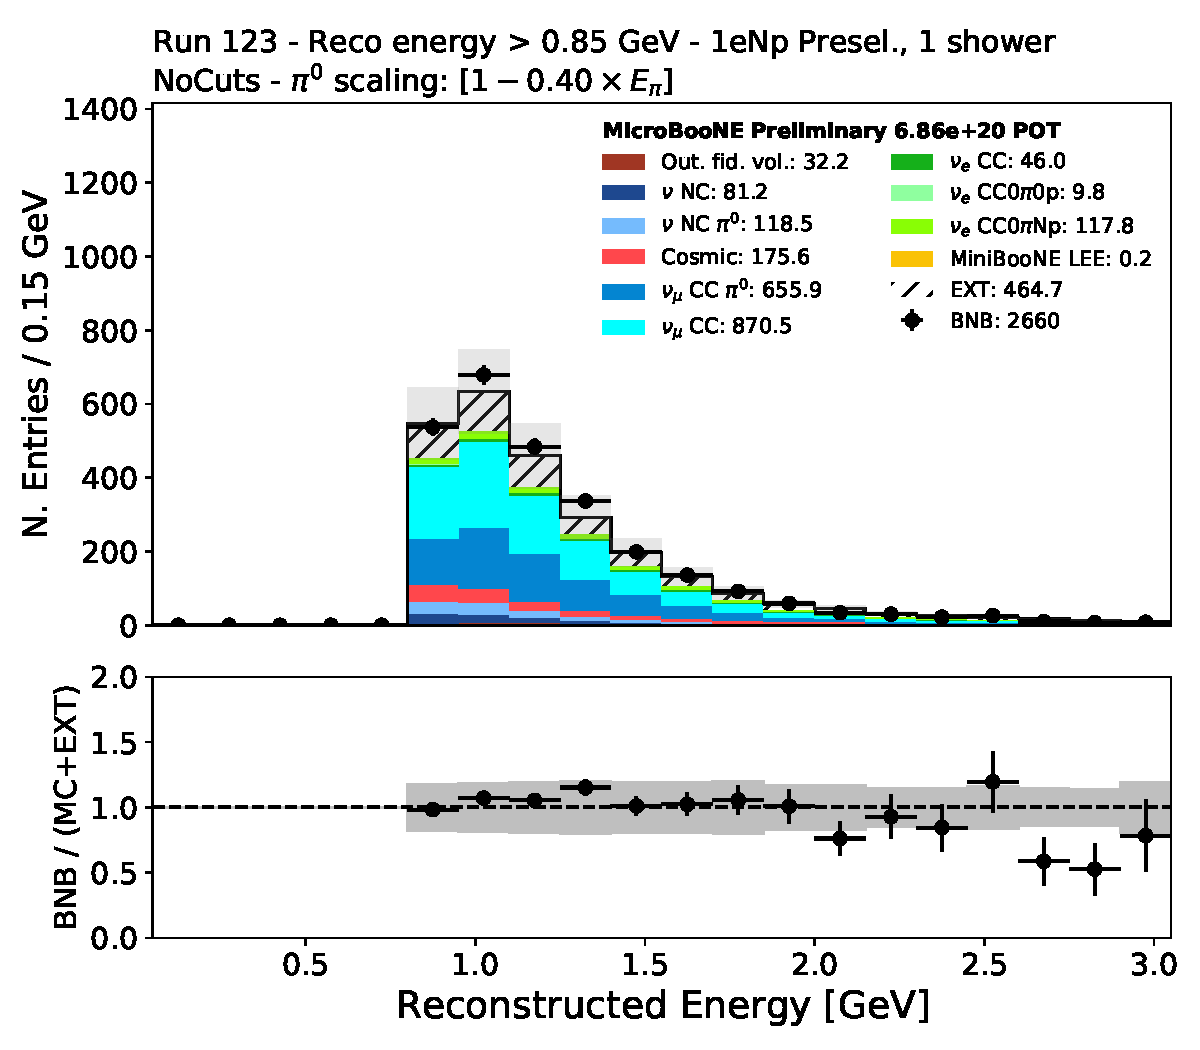
\includegraphics[width=1.00\textwidth]{Sidebands/Figures/1eNp/HighEnergy/HiEext_NPOneShr_None_pi0e040/reco_e_extended.pdf}
    \caption{\npsel Preselection}
    \end{subfigure}
    \begin{subfigure}{0.32\textwidth}
    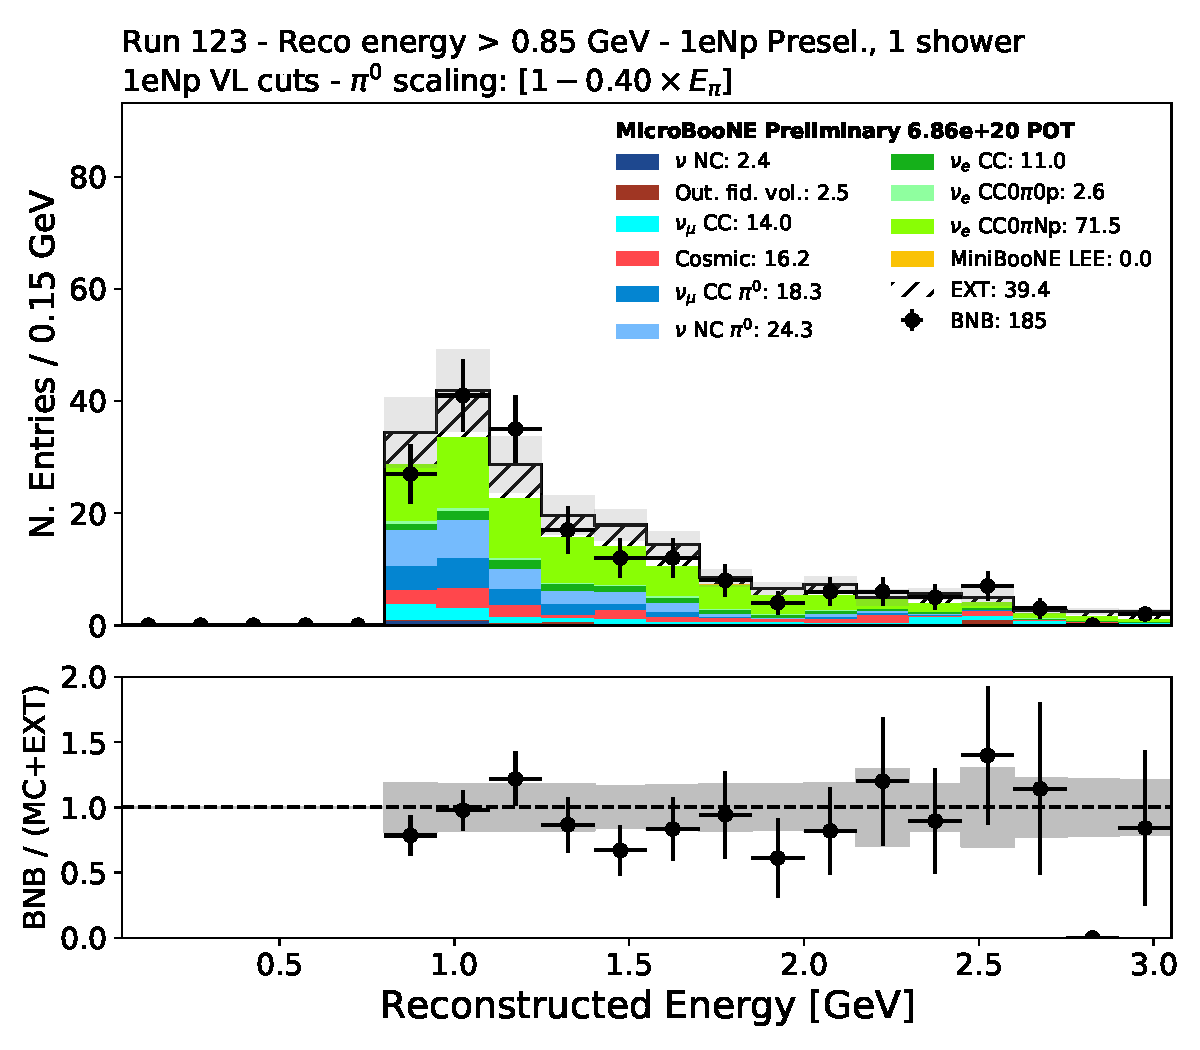
\includegraphics[width=1.00\textwidth]{Sidebands/Figures/1eNp/HighEnergy/HiEext_NPOneShr_NPVL_pi0e040/reco_e_extended.pdf}
    \caption{\npsel VeryLoose cuts}
    \end{subfigure}
    \begin{subfigure}{0.32\textwidth}
    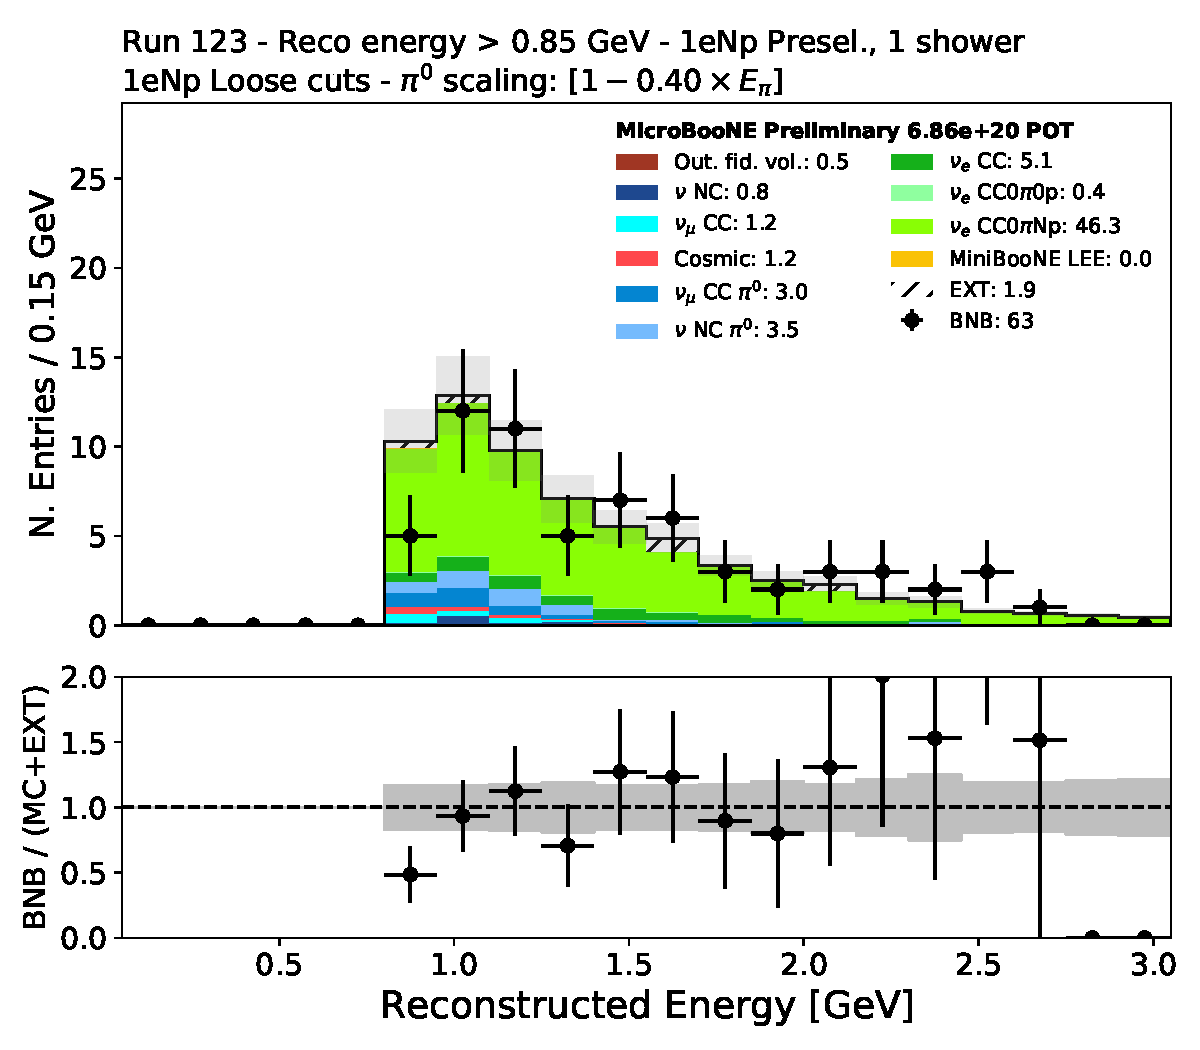
\includegraphics[width=1.00\textwidth]{Sidebands/Figures/1eNp/HighEnergy/HiEext_NPOneShr_NPL_pi0e040/reco_e_extended.pdf}
    \caption{\npsel Loose cuts}
    \end{subfigure}
\caption{\label{fig:sb:1eNp:he:recoe} Reconstructed neutrino energy in the high energy sideband, at different stages of the \npsel selection.}
    \end{center}
\end{figure}

The Loose selection stage in the high energy sideband has a \npsel purity of more than 70\%. Therefore it is ideal to validate the \npsel modeling in terms of the variables that are input to the BDT, as well as the BDT response. Figure~\ref{fig:sb:1eNp:he:L:inputvars} shows the data-MC agreement for some of the most important variables in the selection and the agreement is excellent; for a more complete set of plots at this stage of the selection, see Appendix~\ref{app:datasidebandplotdump:nphe}. The resulting BDT responses are shown in Fig.~\ref{fig:sb:1eNp:he:L:bdtscores} and are in good data-MC agreement. After BDT selection, 36 events survive and event displays indicate that only 2 of them are background (i.e. not \npsel), corresponding to a level of purity (94\%) that is consistent with the expectations.

\begin{figure}[H]
    \begin{center}
    \begin{subfigure}{0.32\textwidth}
    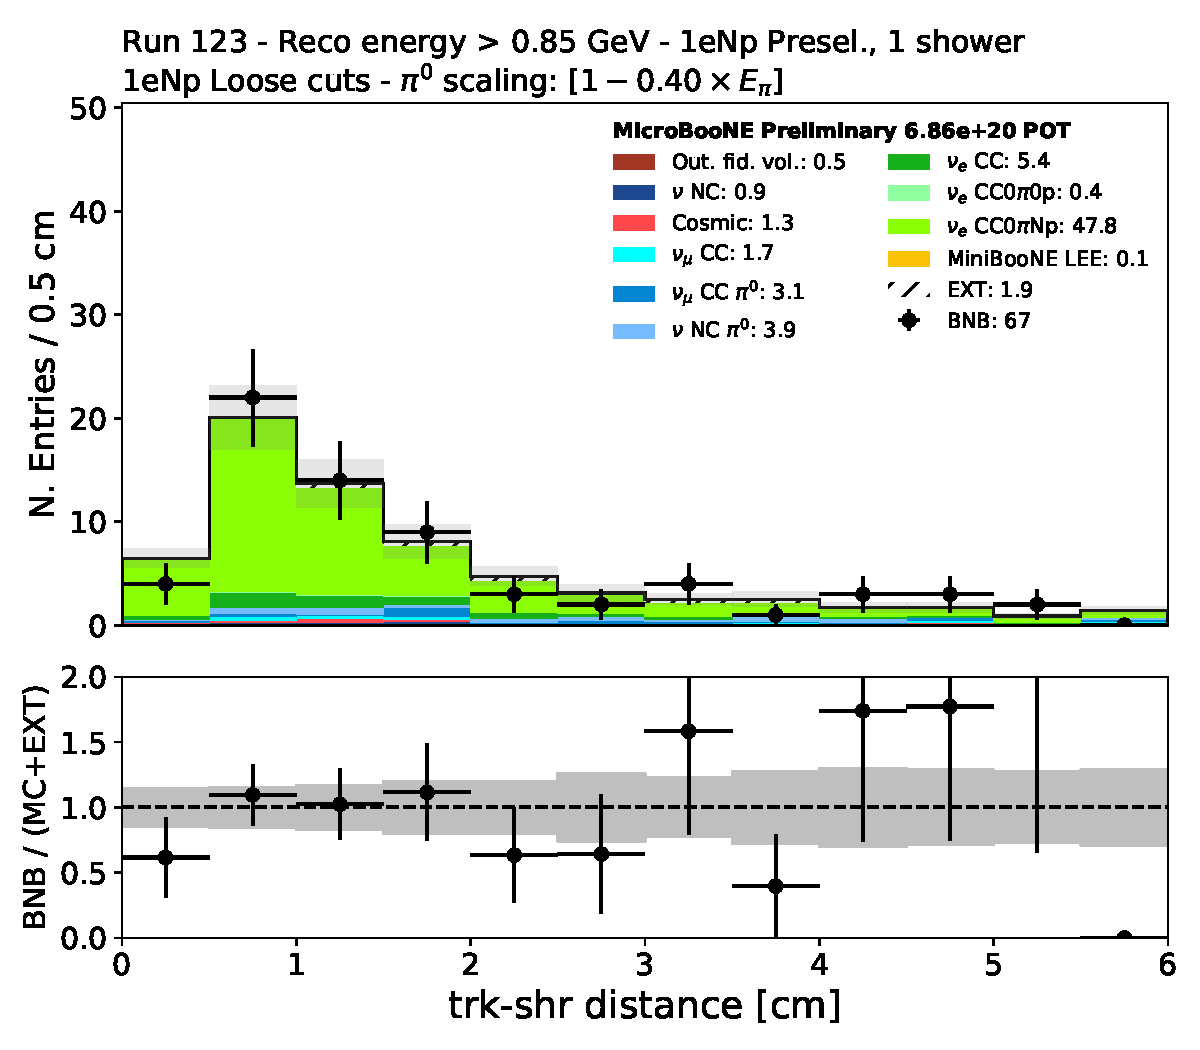
\includegraphics[width=1.00\textwidth]{Sidebands/Figures/1eNp/HighEnergy/HiEext_NPOneShr_NPL_pi0e040/tksh_distance_zoomed.pdf}
    \end{subfigure}
    \begin{subfigure}{0.32\textwidth}
    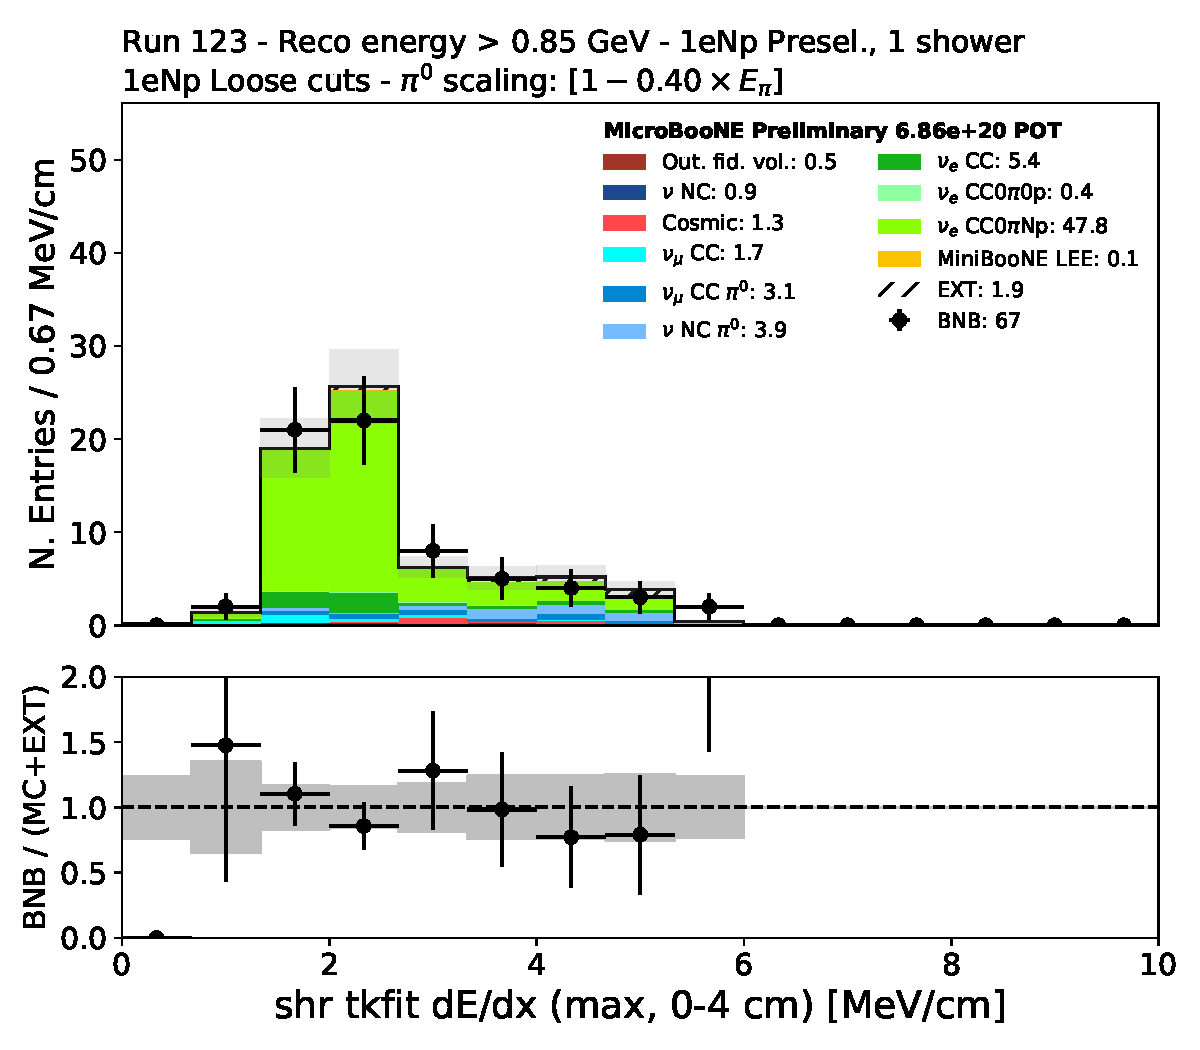
\includegraphics[width=1.00\textwidth]{Sidebands/Figures/1eNp/HighEnergy/HiEext_NPOneShr_NPL_pi0e040/shr_tkfit_dedx_max.pdf}
    \end{subfigure}
    \begin{subfigure}{0.32\textwidth}
    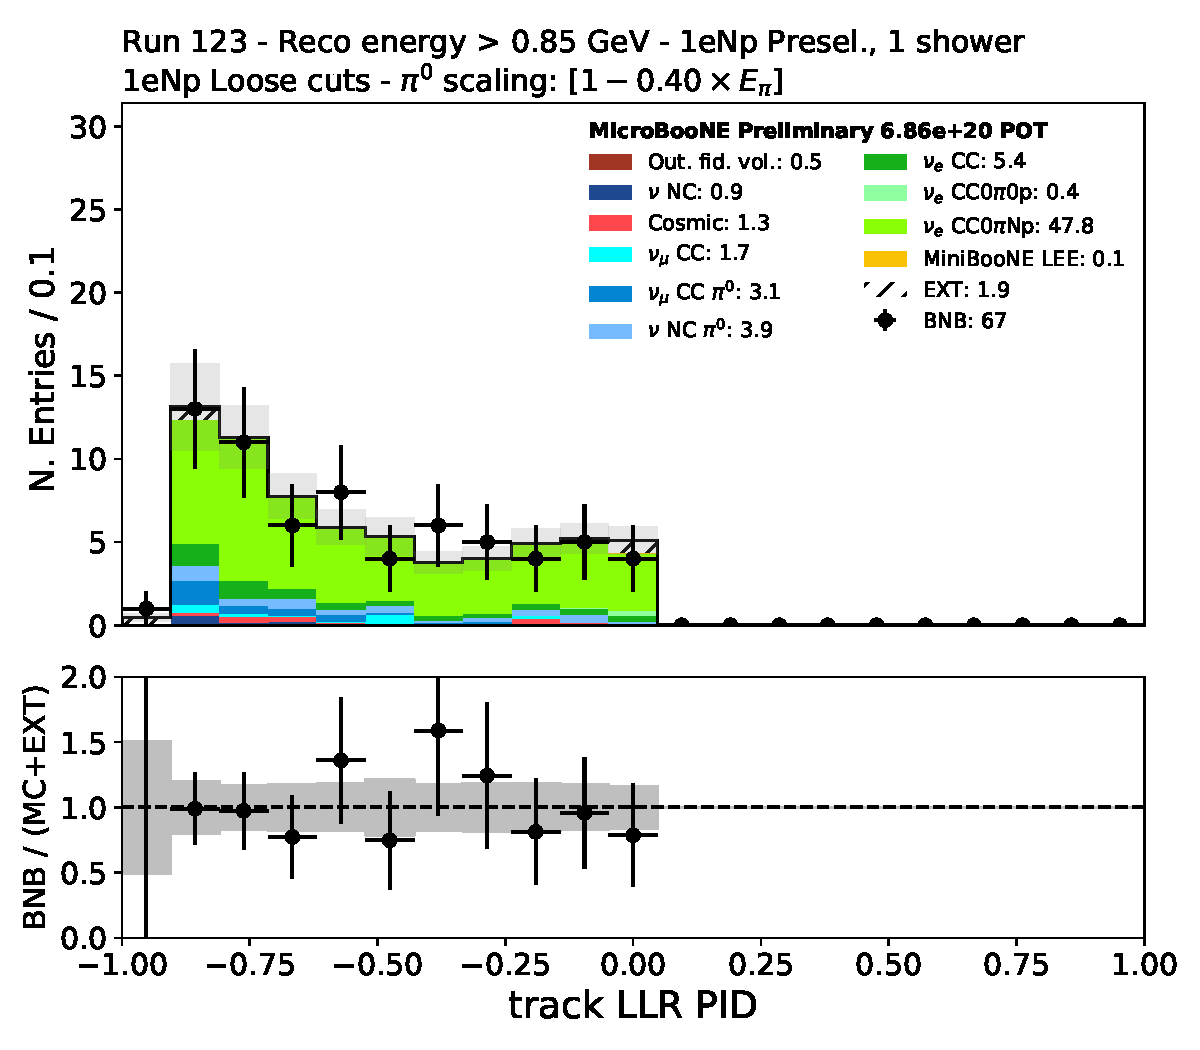
\includegraphics[width=1.00\textwidth]{Sidebands/Figures/1eNp/HighEnergy/HiEext_NPOneShr_NPL_pi0e040/trkpid.pdf}
    \end{subfigure}
\caption{\label{fig:sb:1eNp:he:L:inputvars} Selection of BDT input variables after Loose selection in the \npsel high energy sideband.}
    \end{center}
\end{figure}

\begin{figure}[H]
    \begin{center}
    \begin{subfigure}{0.32\textwidth}
    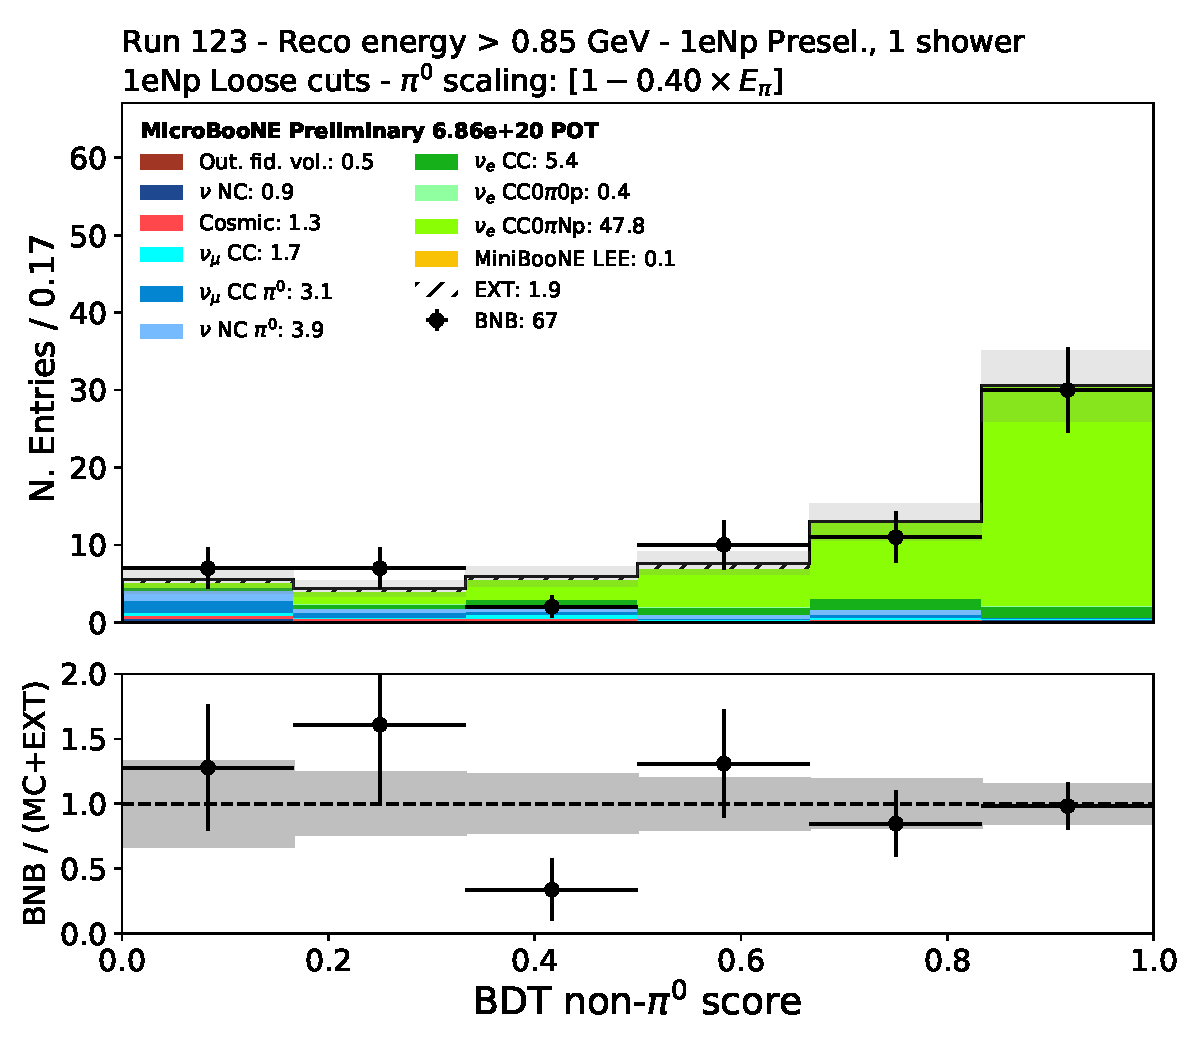
\includegraphics[width=1.00\textwidth]{Sidebands/Figures/1eNp/HighEnergy/HiEext_NPOneShr_NPL_pi0e040/nonpi0_score.pdf}
    \end{subfigure}
    \begin{subfigure}{0.32\textwidth}
    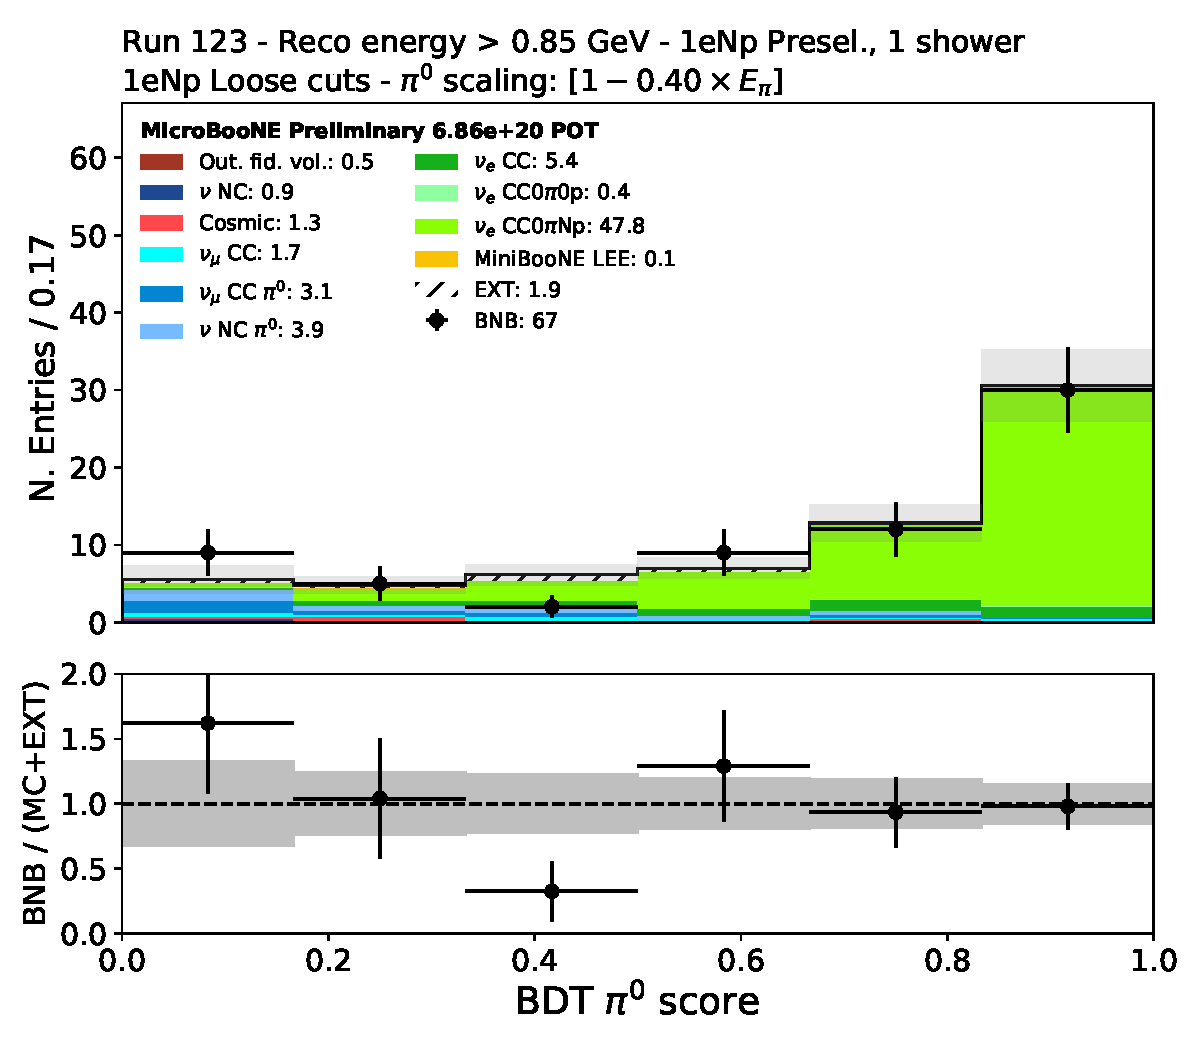
\includegraphics[width=1.00\textwidth]{Sidebands/Figures/1eNp/HighEnergy/HiEext_NPOneShr_NPL_pi0e040/pi0_score.pdf}
    \end{subfigure}
\caption{\label{fig:sb:1eNp:he:L:bdtscores} BDT output after Loose selection in the \npsel high energy sideband.}
    \end{center}
\end{figure}

Since they are not used directly in the selection, kinematic variables are not strongly biased by the selection so they can be used to characterize the selected \nuecc events across a broad phase space. Figure~\ref{fig:sb:1eNp:he:BDT:kinvars} shows a selection of variables and they typically demonstrate good agreement with the expectation. It can be noted that a single bin in the shower $\theta$ angle, corresponding to nearly vertical direction, shows an upward fluctuation. Data events in this bin appear to be well reconstructed and two out of three are \npsel events. Given the low statistics regime no definitive statement can be made about this bin, and it will be monitored when looking at more data.

\begin{figure}[H]
    \begin{center}
    \begin{subfigure}{0.4\textwidth}
    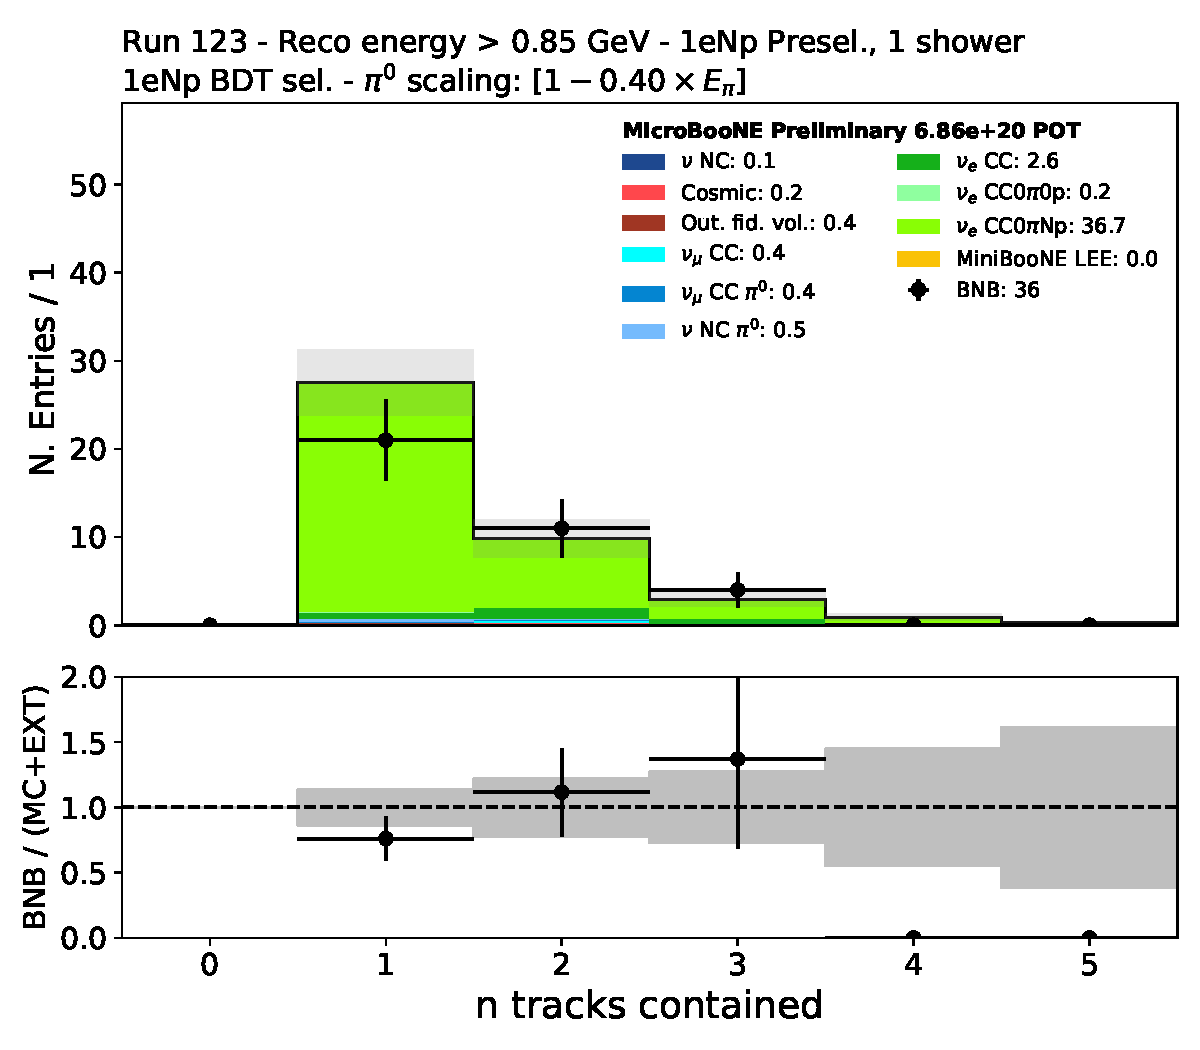
\includegraphics[width=1.00\textwidth]{Sidebands/Figures/1eNp/HighEnergy/HiEext_NPOneShr_NPBDT_pi0e040/n_tracks_contained.pdf}
    \end{subfigure}
    \begin{subfigure}{0.4\textwidth}
    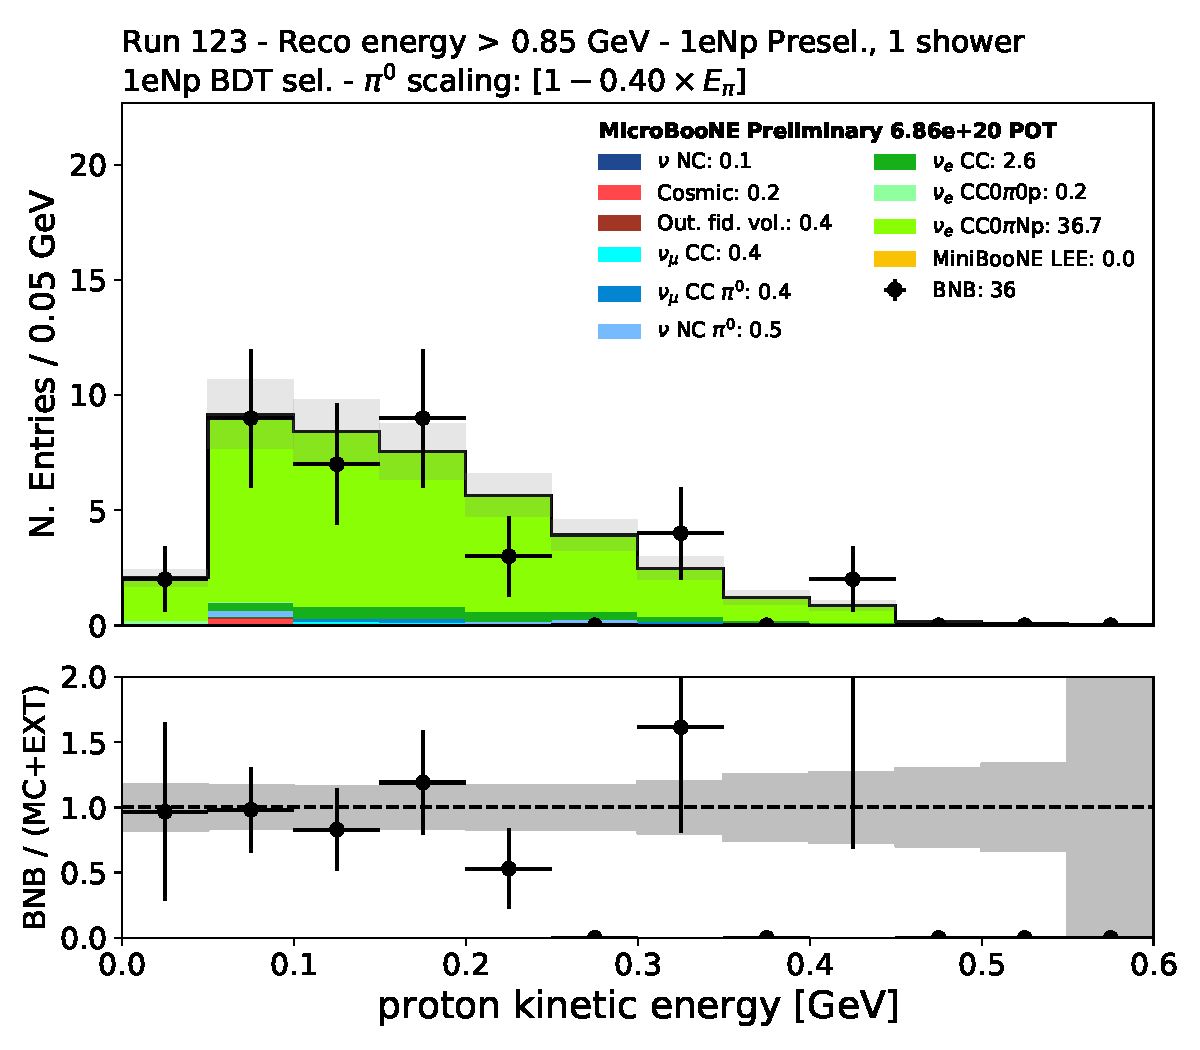
\includegraphics[width=1.00\textwidth]{Sidebands/Figures/1eNp/HighEnergy/HiEext_NPOneShr_NPBDT_pi0e040/protonenergy.pdf}
    \end{subfigure}\\
    \begin{subfigure}{0.4\textwidth}
    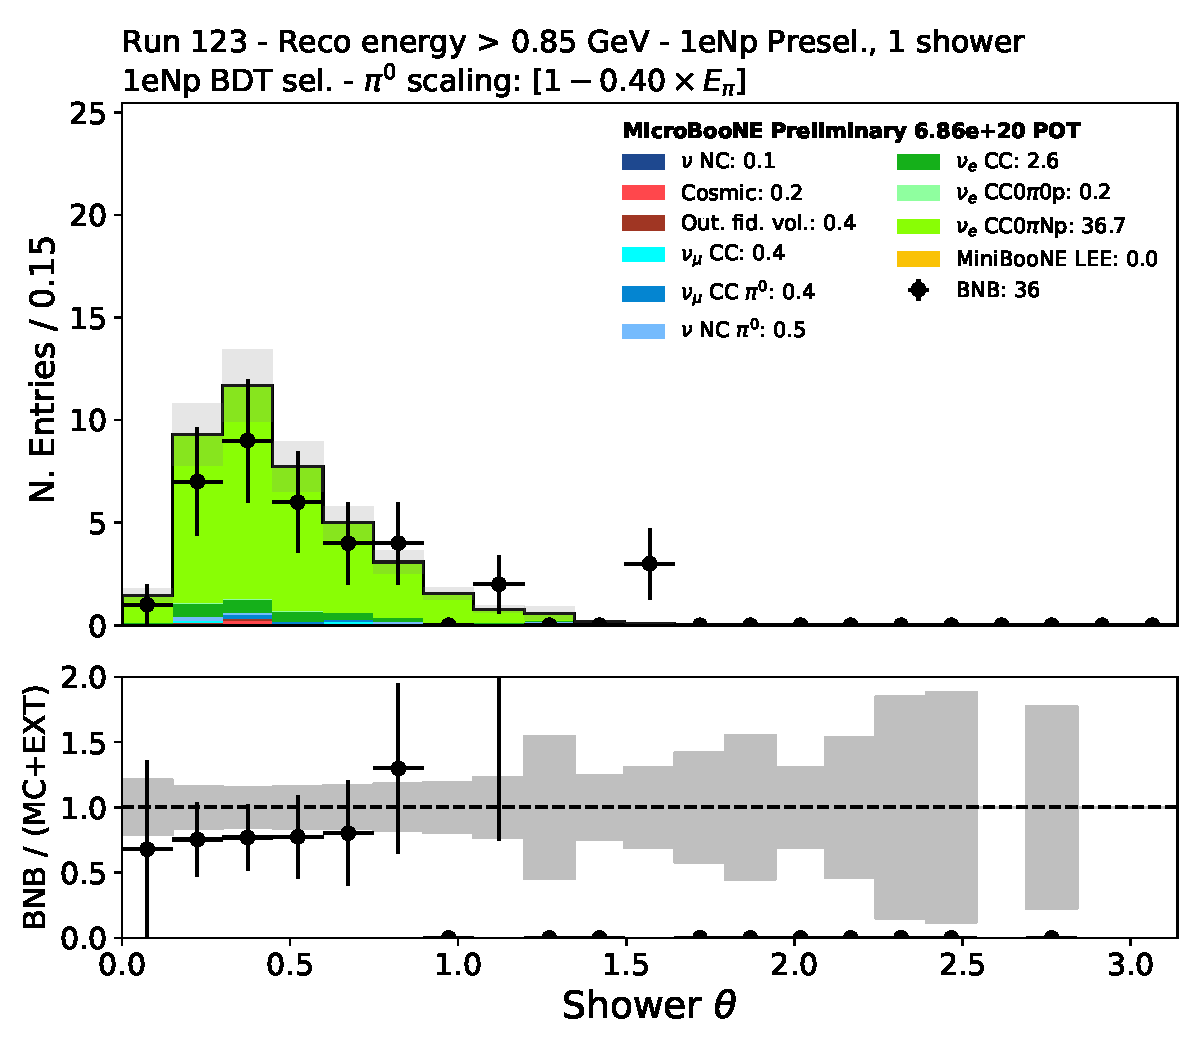
\includegraphics[width=1.00\textwidth]{Sidebands/Figures/1eNp/HighEnergy/HiEext_NPOneShr_NPBDT_pi0e040/shr_theta.pdf}
    \end{subfigure}
    \begin{subfigure}{0.4\textwidth}
    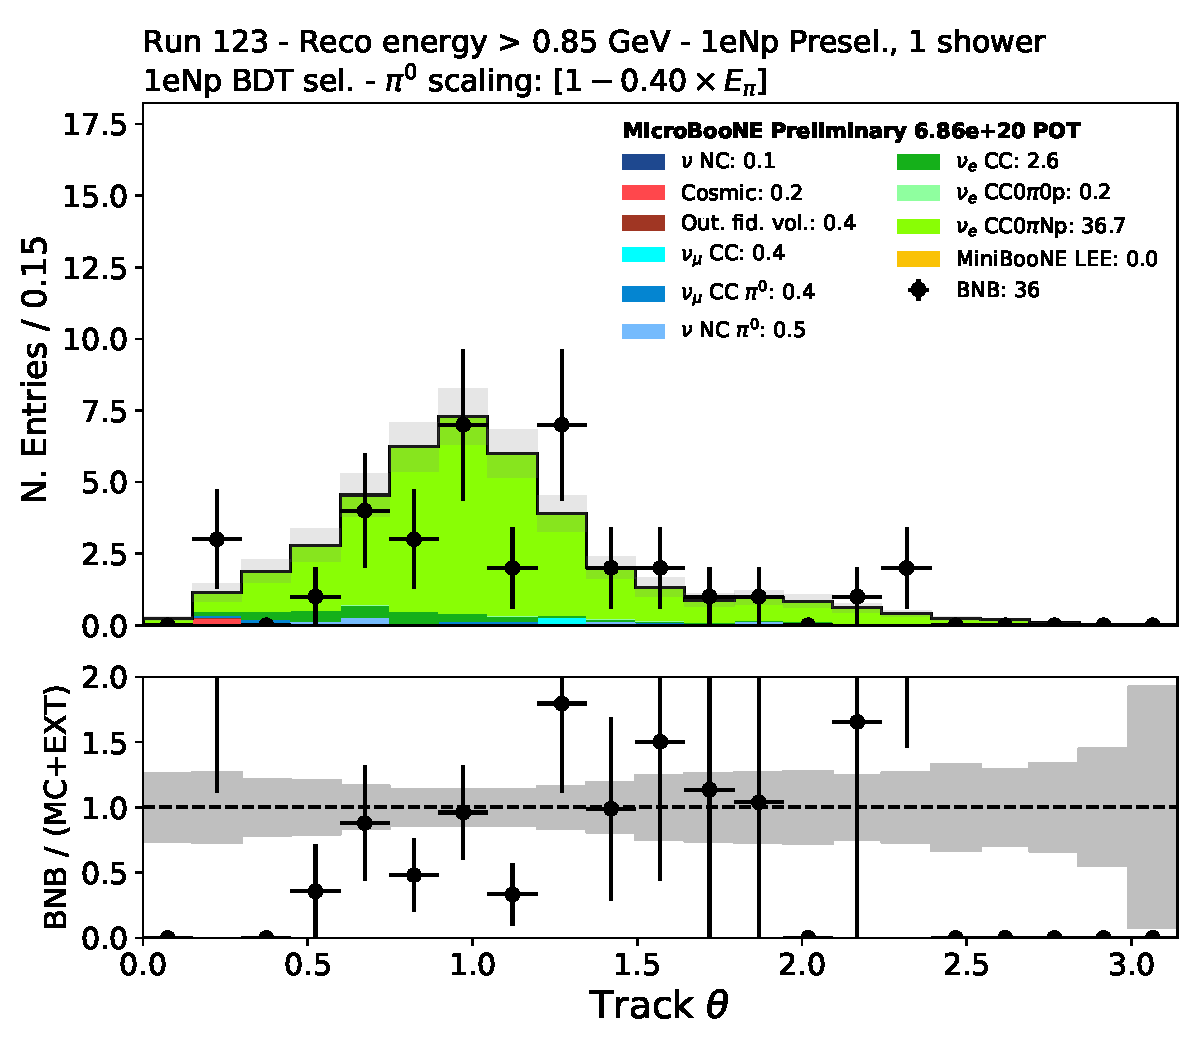
\includegraphics[width=1.00\textwidth]{Sidebands/Figures/1eNp/HighEnergy/HiEext_NPOneShr_NPBDT_pi0e040/trk_theta.pdf}
    \end{subfigure}
\caption{\label{fig:sb:1eNp:he:BDT:kinvars} Selection of kinematic variables after BDT selection in the \npsel high energy sideband.}
    \end{center}
\end{figure}


The results of this sideband demostrate that, at least at high energy, the modeling of the \npsel signal events is accurate both in terms of overall normalization and in terms of the shape of the discriminating variables used in the analysis.

\subsubsection{Low PID Sideband}
\label{sec:sideband:1eNp:lowpid}
The low PID sideband targets the validation of the simulation of the input variables to the BDT, as well as the modeling of background events, using the full energy spectrum.
In this section the distributions of important analysis variables are validated, over the entire energy spectrum, in the low PID region.
This sideband requires, in addition to the \nue pre-selection, exactly one shower contained, and a BDT score less than 0.1. The sideband contains a roughly equal mix of EXT, \numu CC 0$\pi^0$ and \numu $\pi^0$ events and thus is valuebale in helping assess modeling of important backgrounds. Figure~\ref{fig:LPID_1eNp_tkshdist} shows the contribution from \numu and $\pi^0$ events nicely split by track-shower distance, with both contributions well modeled. The data/MC comparisons from this sideband more generally show excellent agreement. We summarize these comparisons with figure~\ref{fig:LPID_1eNp_reco_e} showing the reconstructed energy spectrum after pre-selecion. Plots of all variables input to the \nue selection are presented in appendix~\ref{app:sideband:1eNplowpid}, along with their p-value distributions.

\begin{figure}[H]
    \begin{center}
    \begin{subfigure}{0.45\textwidth}
    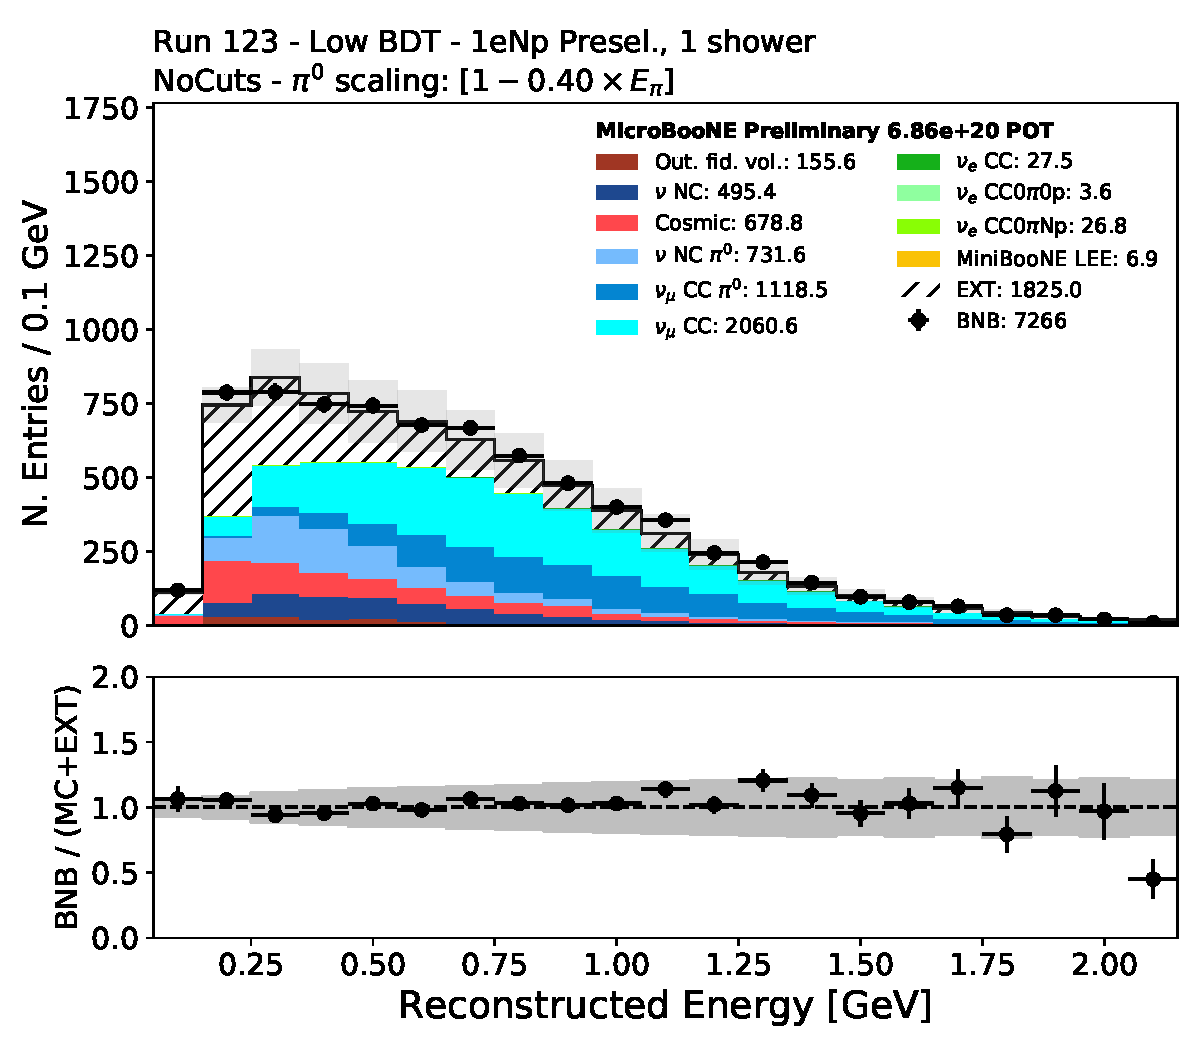
\includegraphics[width=1.00\textwidth]{Sidebands/Figures/1eNp/LPID_NPOneShr_None_pi0e40/reco_e.pdf}
    \caption{\label{fig:LPID_1eNp_reco_e} pre-selection \texttt{reco\_e}}
    \end{subfigure}
    \begin{subfigure}{0.45\textwidth}
    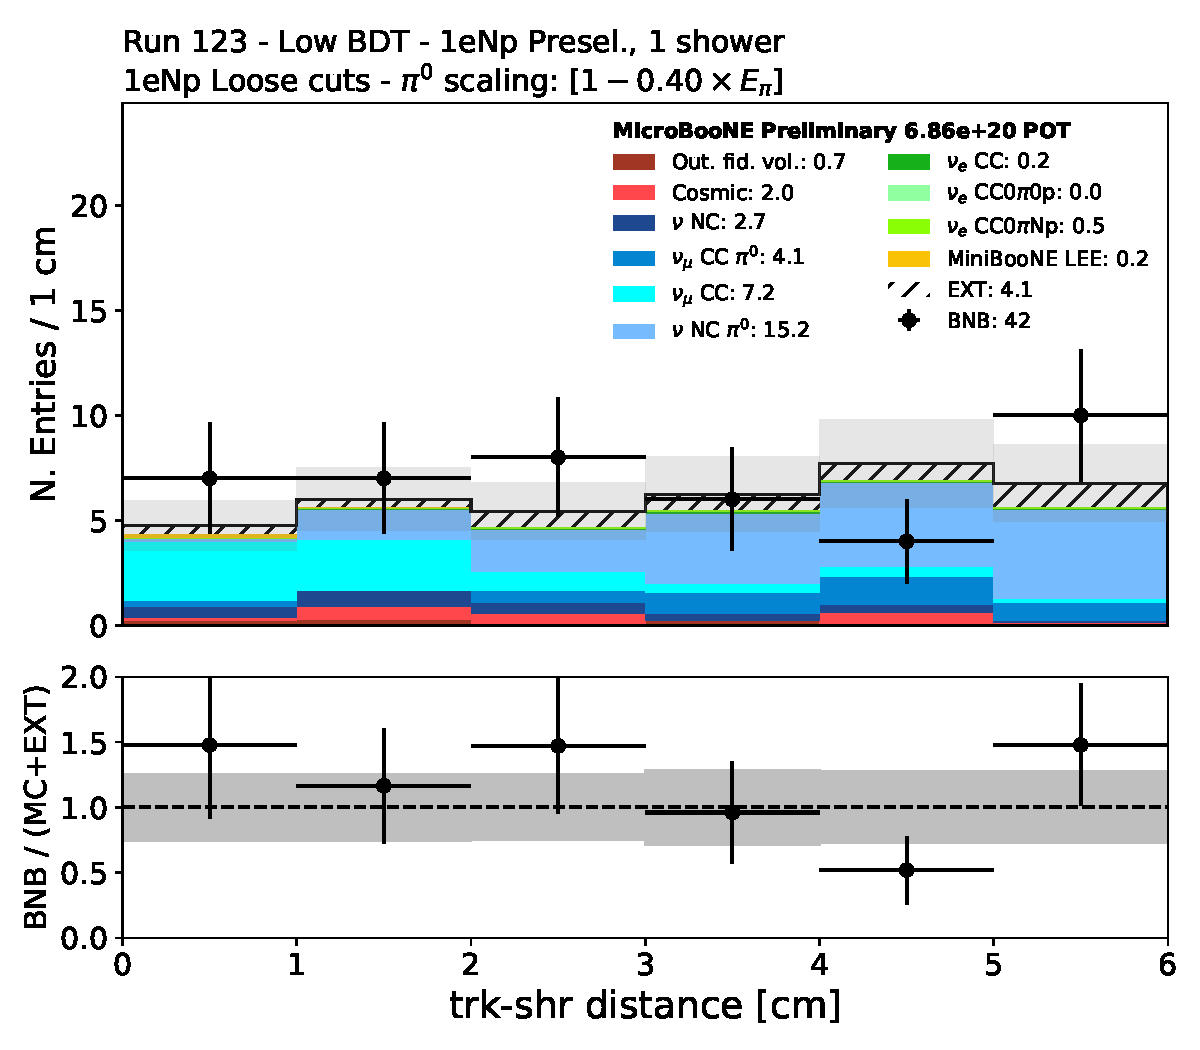
\includegraphics[width=1.00\textwidth]{Sidebands/Figures/1eNp/LPID_NPOneShr_None_pi0e40/tksh_distance_LPID.pdf}
    \caption{\label{fig:LPID_1eNp_tkshdist} loose selection \texttt{tksh\_distance}}
    \end{subfigure}
    \caption{Summary of \npsel low-PID sideband.}
    \end{center}
\end{figure}

\subsubsection{Time Stability Studies}

The results of the \npsel sidebands are analyzed separately for different run periods to check the stability of the data taking quality. Figures~\ref{fig:sb:1eNp:time:twopshr:vl:recoe}-\ref{fig:sb:1eNp:time:he:vl:recoe} show the reconstructed neutrino energy in the three run periods for the three sidebands analyzed; plots are shown after VeryLoose selection which guarantees enough statistics for a meaningful comparison. The consistence between all runs is satisfactory.

\begin{figure}[H]
    \begin{center}
    \begin{subfigure}{0.32\textwidth}
    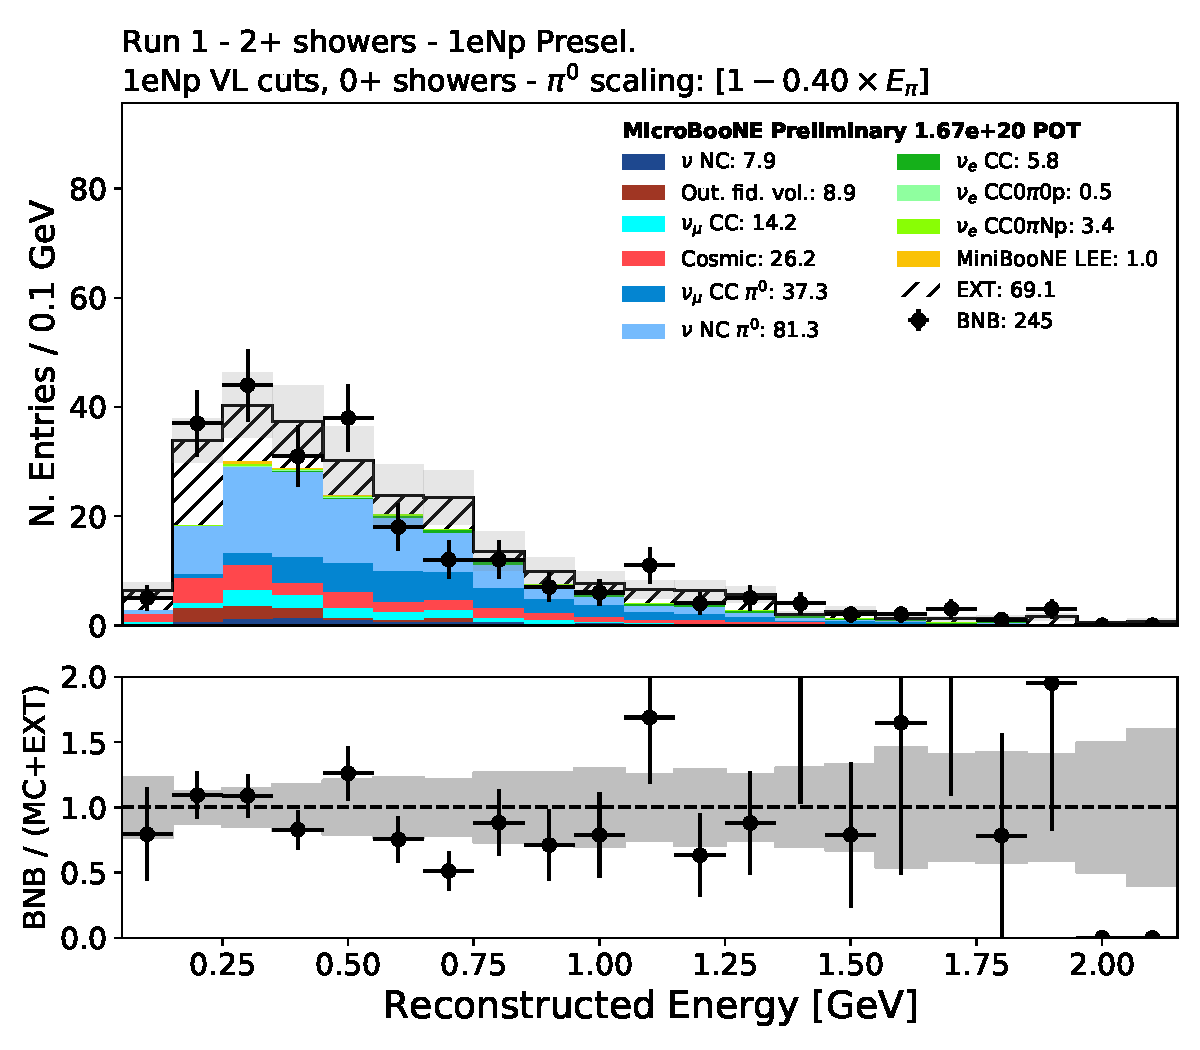
\includegraphics[width=1.00\textwidth]{Sidebands/Figures/1eNp/TimeDependence/reco_e_TwoPShr_NPVL_Run1.pdf}
    \caption{Run1}
    \end{subfigure}
    \begin{subfigure}{0.32\textwidth}
    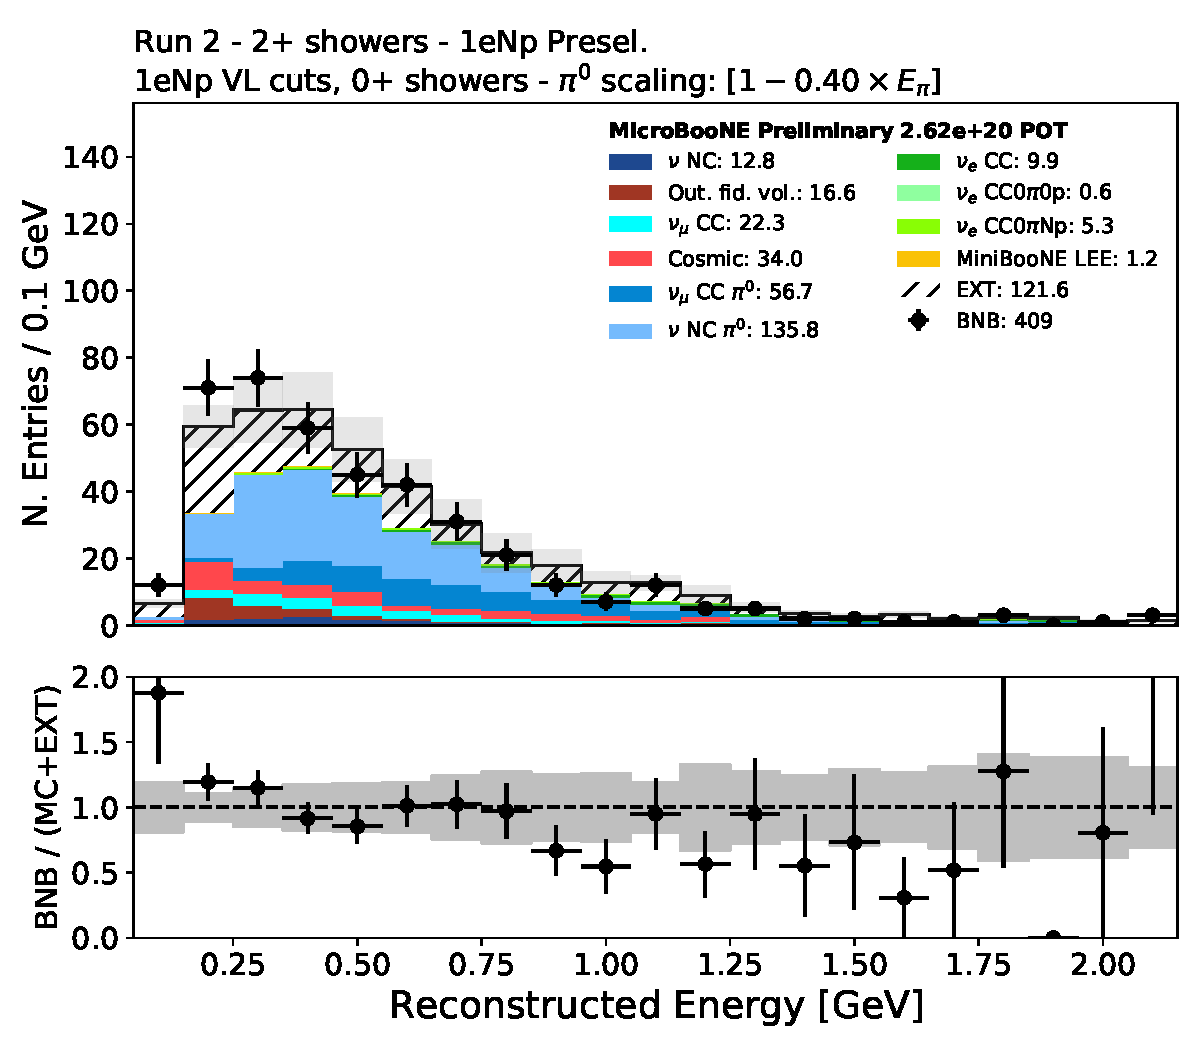
\includegraphics[width=1.00\textwidth]{Sidebands/Figures/1eNp/TimeDependence/reco_e_TwoPShr_NPVL_Run2.pdf}
    \caption{Run2}
    \end{subfigure}
    \begin{subfigure}{0.32\textwidth}
    \includegraphics[width=1.00\textwidth]{Sidebands/Figures/1eNp/TimeDependence/reco_e_TwoPShr_NPVL_Run3.pdf}
    \caption{Run3}
    \end{subfigure}
    \caption{\label{fig:sb:1eNp:time:twopshr:vl:recoe} Reconstructed neutrino energy in the \npsel 2+ shower sideband after VeryLoose selection in the three data taking periods analyzed.}
    \end{center}
\end{figure}

\begin{figure}[H]
    \begin{center}
    \begin{subfigure}{0.32\textwidth}
    \includegraphics[width=1.00\textwidth]{Sidebands/Figures/1eNp/TimeDependence/reco_e_LPID_NPVL_Run1.pdf}
    \caption{Run1}
    \end{subfigure}
    \begin{subfigure}{0.32\textwidth}
    \includegraphics[width=1.00\textwidth]{Sidebands/Figures/1eNp/TimeDependence/reco_e_LPID_NPVL_Run2.pdf}
    \caption{Run2}
    \end{subfigure}
    \begin{subfigure}{0.32\textwidth}
    \includegraphics[width=1.00\textwidth]{Sidebands/Figures/1eNp/TimeDependence/reco_e_LPID_NPVL_Run3.pdf}
    \caption{Run3}
    \end{subfigure}
    \caption{\label{fig:sb:1eNp:time:lpid:vl:recoe} Reconstructed neutrino energy in the \npsel 2+ shower sideband after VeryLoose selection in the three data taking periods analyzed.}
    \end{center}
\end{figure}

\begin{figure}[H]
    \begin{center}
    \begin{subfigure}{0.32\textwidth}
    \includegraphics[width=1.00\textwidth]{Sidebands/Figures/1eNp/TimeDependence/reco_e_coarse_HE_NPVL_Run1.pdf}
    \caption{Run1}
    \end{subfigure}
    \begin{subfigure}{0.32\textwidth}
    \includegraphics[width=1.00\textwidth]{Sidebands/Figures/1eNp/TimeDependence/reco_e_coarse_HE_NPVL_Run2.pdf}
    \caption{Run2}
    \end{subfigure}
    \begin{subfigure}{0.32\textwidth}
    \includegraphics[width=1.00\textwidth]{Sidebands/Figures/1eNp/TimeDependence/reco_e_coarse_HE_NPVL_Run3.pdf}
    \caption{Run3}
    \end{subfigure}
    \caption{\label{fig:sb:1eNp:time:he:vl:recoe} Reconstructed neutrino energy in the \npsel high energy sideband after VeryLoose selection in the three data taking periods analyzed.}
    \end{center}
\end{figure}

It is worth pointing out that a large deficit in the high energy sideband in Run3 after BDT selection was initially observed. This deficit triggered numerous studies (see e.g. Sec.~\ref{sec:timestability}) that were not able to identify a detector state change that could be responsible for this deficit. After including the recovery algorithms (see Sec.~\ref{sec:sideband:recovery}), the number of events in this sample doubled, with the effect of a significant mitigation of the deficit. The reconstructed neutrino energy distributions for all runs in the high energy \npsel sideband after BDT selection are shown in Fig.~\ref{fig:sb:1eNp:time:he:bdt:recoe}, which includes also a comparison of before and after the inclusion of the recovery algorithms in Run3.

\begin{figure}[H]
    \begin{center}
    \begin{subfigure}{0.4\textwidth}
    \includegraphics[width=1.00\textwidth]{Sidebands/Figures/1eNp/TimeDependence/reco_e_coarse_HE_NPBDT_Run1.pdf}
    \caption{Run1}
    \end{subfigure}
    \begin{subfigure}{0.4\textwidth}
    \includegraphics[width=1.00\textwidth]{Sidebands/Figures/1eNp/TimeDependence/reco_e_coarse_HE_NPBDT_Run2.pdf}
    \caption{Run2}
    \end{subfigure}\\
    \begin{subfigure}{0.4\textwidth}
    \includegraphics[width=1.00\textwidth]{Sidebands/Figures/1eNp/TimeDependence/reco_e_coarse_HE_NPBDT_Run3.pdf}
    \caption{Run3}
    \end{subfigure}
    \begin{subfigure}{0.4\textwidth}
    \includegraphics[width=1.00\textwidth]{Sidebands/Figures/1eNp/TimeDependence/reco_e_coarse_HE_NPBDT_Run3_noRecAlg.png}
    \caption{Run3, before recovery algorithms}
    \end{subfigure}
    \caption{\label{fig:sb:1eNp:time:he:bdt:recoe} Reconstructed neutrino energy in the \npsel high energy sideband after VeryLoose selection in the three data taking periods analyzed.}
    \end{center}
\end{figure}

\subsubsection{Event Displays}

This section shows a selection of event displays among the events that pass the BDT selection in the \npsel sidebands described above. For a more complete set of event displays, see Docdb 30666. 

Representative event displays from the \npsel 2+ shower sideband are shown in Fig.~\ref{fig:sb:1eNp:twopshr:evd}. Two of them (a, b) show nice NC$\pi^0$ candidates at medium-low energy, where one of the showers is attached to the vertex; event display (c) is most likely a CC$\pi^0$ event where the muon (with Michel) is mis-reconstructed as the shower attached to the vertex, and one of the $\pi^0$ showers is also reconstructed; the last one (d) is a $\nu_e$ event where the electron shower is split so that the event falls in the 2+ shower sideband.

\begin{figure}[H]
    \begin{center}
    \begin{subfigure}{0.45\textwidth}
    \includegraphics[width=1.00\textwidth]{Sidebands/Figures/1eNp/TwoShower/EVD/evt-17119-1-59_reco2.png}
    \caption{Event 17119/1/59. NC$\pi^0$, $E_\nu^{\texttt{reco}} = 0.52~\texttt{GeV}$.}
    \end{subfigure}
    \begin{subfigure}{0.45\textwidth}
    \includegraphics[width=1.00\textwidth]{Sidebands/Figures/1eNp/TwoShower/EVD/evt-9060-124-6212_reco2.png}
    \caption{Event 9060/124/6212. NC$\pi^0$, $E_\nu^{\texttt{reco}} = 0.72~\texttt{GeV}$.}
    \end{subfigure} \\
    \vspace{0.3cm}
    \begin{subfigure}{0.45\textwidth}
    \includegraphics[width=1.00\textwidth]{Sidebands/Figures/1eNp/TwoShower/EVD/evt-14073-207-10357_reco1.png}
    \caption{Event 14073/207/10357. CC$\pi^0$, $E_\nu^{\texttt{reco}} = 0.66~\texttt{GeV}$.}
    \end{subfigure}
    \begin{subfigure}{0.45\textwidth}
    \includegraphics[width=1.00\textwidth]{Sidebands/Figures/1eNp/TwoShower/EVD/evt-15289-10-502_reco.png}
    \caption{Event 15289/10/502. $1e1p$, $E_\nu^{\texttt{reco}} = 0.85~\texttt{GeV}$.}
    \end{subfigure}
    \caption{\label{fig:sb:1eNp:twopshr:evd} Selected event displays for the \npsel 2+ shower sideband. All events pass the BDT selection.}
    \end{center}
\end{figure}

Representative event displays from the \npsel high energy sideband are shown in Fig.~\ref{fig:sb:1eNp:he:evd}. They are all \npsel events, which confirms the expected high purity of our selection. Both the electron shower and the hadronic part of the interaction seem well reconstructed.

\begin{figure}[H]
    \begin{center}
    \begin{subfigure}{0.45\textwidth}
    \includegraphics[width=1.00\textwidth]{Sidebands/Figures/1eNp/HighEnergy/EVD/evt-5161-8-447_reco2.png}
    \caption{Event 5161-8-447. $1e1p$, $E_\nu^{\texttt{reco}} = 1.1~\texttt{GeV}$.}
    \end{subfigure}
    \begin{subfigure}{0.45\textwidth}
    \includegraphics[width=1.00\textwidth]{Sidebands/Figures/1eNp/HighEnergy/EVD/evt-8799-142-7129_reco2.png}
    \caption{Event 8799-142-7129. $1e3p$, $E_\nu^{\texttt{reco}} = 1.5~\texttt{GeV}$.}
    \end{subfigure} \\
    \vspace{0.3cm}
    \begin{subfigure}{0.45\textwidth}
    \includegraphics[width=1.00\textwidth]{Sidebands/Figures/1eNp/HighEnergy/EVD/evt-8936-51-2567_reco2.png}
    \caption{Event 8936-51-2567. $1e2p$, $E_\nu^{\texttt{reco}} = 1.7~\texttt{GeV}$.}
    \end{subfigure}
    \begin{subfigure}{0.45\textwidth}
    \includegraphics[width=1.00\textwidth]{Sidebands/Figures/1eNp/HighEnergy/EVD/evt-9207-118-5940_reco2.png}
    \caption{Event 9207-118-5940. $1e2p$, $E_\nu^{\texttt{reco}} = 1.2~\texttt{GeV}$.}
    \end{subfigure}
    \caption{\label{fig:sb:1eNp:he:evd} Selected event displays for the \npsel high energy sideband. All events pass the BDT selection.}
    \end{center}
\end{figure}

A few additional raw event displays from the \npsel high-energy sideband are shown in figure~\ref{fig:sb:1eNp:he:evd:raw}.

\begin{figure}[H]
    \begin{center}
    \begin{subfigure}{0.45\textwidth}
    \includegraphics[width=1.00\textwidth]{Sidebands/Figures/1eNp/HighEnergy/EVD/raw/10704_168_8406_Y_raw.png}
    \caption{Event 10704-168-8406.}
    \end{subfigure}
    \begin{subfigure}{0.45\textwidth}
    \includegraphics[width=1.00\textwidth]{Sidebands/Figures/1eNp/HighEnergy/EVD/raw/10846_207_10366_Y_raw.png}
    \caption{Event 10846-207-10366.}
    \end{subfigure} \\
    \vspace{0.3cm}
    \begin{subfigure}{0.45\textwidth}
    \includegraphics[width=1.00\textwidth]{Sidebands/Figures/1eNp/HighEnergy/EVD/raw/14034_17_890_Y_raw.png}
    \caption{Event 14034-17-890.}
    \end{subfigure}
    \begin{subfigure}{0.45\textwidth}
    \includegraphics[width=1.00\textwidth]{Sidebands/Figures/1eNp/HighEnergy/EVD/raw/3633_6046_72_Y_raw.png}
    \caption{Event 3633-6046-72.}
    \end{subfigure}
    \caption{\label{fig:sb:1eNp:he:evd:raw} Selected event displays for the \npsel high energy sideband. All events pass the BDT selection.}
    \end{center}
\end{figure}
\subsection{1e0p Sidebands}
\label{sec:sideband:1e0p}

%\begin{comment}
\subsubsection{Two+ Shower Sideband}
\label{sec:sideband:1e0p:2pshr}

The two or more shower sideband is defined by a set of pre-selection cuts common to the $\nu_e$ search, no requirement on the number of contained tracks, and a minimum of two contained showers. This data set is mostly populated with $\pi^0$ interactions, so this allows for the study of $\pi^0$ modelling at each step of the analysis.

The visible reconstructed energy at several stages of the analysis is shown in \cref{fig:sb:1eZp:twopshr:recoe}. The stages shown are: the \zpsel preselection, the \zpsel loose cuts and the \zpsel BDT selection. Good agreement between data and simulation is observed. After the BDT selection, 7 data events remain and 5.3 are predicted.

\begin{figure}[H]
    %\begin{center}
    \centering
    \begin{subfigure}{0.3\textwidth}
    %\centering
    \includegraphics[width=1.00\textwidth]{Sidebands/Figures/TwoShr_1e0pSel_newSamples/reco_e_presel.pdf}
    \caption{\zpsel Preselection}
    \end{subfigure}
    \begin{subfigure}{0.3\textwidth}
    %\centering
    \includegraphics[width=1.00\textwidth]{Sidebands/Figures/TwoShr_1e0pSel_newSamples/reco_e_loose.pdf}
    \caption{\zpsel Loose cuts}
    \end{subfigure}
    \begin{subfigure}{0.3\textwidth}
    %\centering
    \includegraphics[width=1.00\textwidth]{Sidebands/Figures/TwoShr_1e0pSel_newSamples/reco_e_BDT.pdf}
    \caption{\zpsel BDT selection}
    \end{subfigure}
    \caption{\label{fig:sb:1eZp:twopshr:recoe} Reconstructed neutrino energy in the 2+ shower sideband, at different stages of the \zpsel selection.}
    %\end{center}
\end{figure}

Figure~\ref{fig:sb:1eZp:twopshr:loose:vars1} shows select data-MC comparisons of NC \pizero rich distributions from the 2+ shower \zpsel sideband, all demonstrating good data/MC agreement. Figure~\ref{fig:sb:1eZp:twopshr:loose:bdt} shows the BDT response in this sideband. Additional data/MC comparisons from this sideband are included in appendix~\ref{app:sideband:1e0ptwoplusshower}, along with a summary of p-values.

\begin{figure}[H]
    \begin{center}
    \begin{subfigure}{0.4\textwidth}
    \includegraphics[width=1.00\textwidth]{Sidebands/Figures/TwoShr_1e0pSel_newSamples/secondshower_Y_nhit_loose.pdf}
    %\caption{}
    \end{subfigure}
    \begin{subfigure}{0.4\textwidth}
    \includegraphics[width=1.00\textwidth]{Sidebands/Figures/TwoShr_1e0pSel_newSamples/subcluster_loose.pdf}
    %\caption{}
    \end{subfigure} \\
    \begin{subfigure}{0.4\textwidth}
    \includegraphics[width=1.00\textwidth]{Sidebands/Figures/TwoShr_1e0pSel_newSamples/shr_tkfit_gap10_dedx_Y_loose.pdf}
    %\caption{}
    \end{subfigure}
    \begin{subfigure}{0.4\textwidth}
    \includegraphics[width=1.00\textwidth]{Sidebands/Figures/TwoShr_1e0pSel_newSamples/shrmoliereavg_loose.pdf}
    %\caption{}
    \end{subfigure}
    \caption{\label{fig:sb:1eZp:twopshr:loose:vars1} Selection variables after \zpsel Loose cuts in the 2+ shower sideband.}
    \end{center}
\end{figure}

\begin{figure}[H]
    \begin{center}
    \begin{subfigure}{0.4\textwidth}
    \includegraphics[width=1.00\textwidth]{Sidebands/Figures/TwoShr_1e0pSel_newSamples/bkg_score_loose.pdf}
    %\caption{}
    \end{subfigure}
    \caption{\label{fig:sb:1eZp:twopshr:loose:bdt} BDT response after \zpsel loose cuts in the 2+ shower sideband.}
    \end{center}
\end{figure}


%\end{comment}
\subsubsection{High Energy Sideband}
\label{sec:sideband:1e0p:he}
The high energy sideband for the 1e0p selection is defined as events above 0.9 GeV in reconstructed neutrino energy.  These events were used to validate the input variables on electron neutrino events at high energy at various selection stages: pre-selection, loose selection and BDT selection. 

Fig.~\ref{fig:1e0p:High_E_sideband:reco_e} shows the reconstructed neutrino energy at pre-selection, loose selection, and after the BDT selection. The data in these distributions agree well with the prediction. 

\begin{figure}[H]
    \centering
    \begin{subfigure}{0.3\textwidth}
    \includegraphics[width=1.0\textwidth]{1e0p/High_E_Sideband/reco_e_extended.pdf}
    \caption{Pre-Selection}
    \end{subfigure}
    \begin{subfigure}{0.3\textwidth}
    \includegraphics[width=1.0\textwidth]{1e0p/High_E_Sideband/loose_selection/reco_e_extended.pdf}
    \caption{Loose Selection}
    \end{subfigure}
    \begin{subfigure}{0.3\textwidth}
    \includegraphics[width=1.0\textwidth]{1e0p/High_E_Sideband/BDT_selection/reco_e_highe.pdf}
    \caption{BDT Selection}
    \end{subfigure}
    \caption{Reconstructed energy in the high energy sideband at different selection stages.} 
    \label{fig:1e0p:High_E_sideband:reco_e}
\end{figure}

After loose selection 35 events remain, reducing the expected cosmic background by 96\% and the $\pi^{0}$ background by about half.  

One of the BDT selection variables that is able to well separate electrons and pi0s is dE/dx on the Y plane calculated for four centimeters starting one centeimeter away from the shower start point. Fig.~\ref{fig:1e0p:High_E_sideband:dedx} shows the shower dE/dx and $e$/$\gamma$ separation in the high energy side band after pre-selection, loose selection and BDT selection.

\begin{figure}[H]
    \centering
    \begin{subfigure}{0.3\textwidth}
    \includegraphics[width=1.0\textwidth]{1e0p/High_E_Sideband/shr_tkfit_gap10_dedx_Y.pdf}
    \caption{Pre-Selection}
    \end{subfigure}
    \begin{subfigure}{0.3\textwidth}
    \includegraphics[width=1.0\textwidth]{1e0p/High_E_Sideband/loose_selection/shr_tkfit_gap10_dedx_Y.pdf}
    \caption{Loose Selection}
    \end{subfigure}
    \begin{subfigure}{0.3\textwidth}
    \includegraphics[width=1.0\textwidth]{1e0p/High_E_Sideband/BDT_selection/shr_tkfit_gap10_dedx_Y.pdf}
    \caption{BDT Selection}
    \end{subfigure}
    \caption{dE/dx in the high energy sideband at different selection stages.} 
    \label{fig:1e0p:High_E_sideband:dedx}
\end{figure}

The shower dE/dx and many other variables are used in the BDT that is ultimately used to select 1e0p events. 
Fig.~\ref{fig:1e0p:High_E_sideband:bdtscore} shows the background BDT score at pre-selection, loose selection, and after the BDT selection.  
\begin{figure}[H]
    \centering
    \begin{subfigure}{0.3\textwidth}
    \includegraphics[width=1.0\textwidth]{1e0p/High_E_Sideband/bkg_score.pdf}
    \caption{Pre-Selection}
    \end{subfigure}
    \begin{subfigure}{0.3\textwidth}
    \includegraphics[width=1.0\textwidth]{1e0p/High_E_Sideband/loose_selection/bkg_score.pdf}
    \caption{Loose Selection}
    \end{subfigure}
    \begin{subfigure}{0.3\textwidth}
    \includegraphics[width=1.0\textwidth]{1e0p/High_E_Sideband/BDT_selection/bkg_score_high_bdt.pdf}
    \caption{BDT Selection}
    \end{subfigure}
    \caption{BDT score in the high energy side band at different selection stages.} 
    \label{fig:1e0p:High_E_sideband:bdtscore}
\end{figure}

A full set of plots of the variables used as BDT inputs or in the loose selection, at the pre-selection stage, can be found in Section~\ref{sec:zpHighE_plots}. Good Data-MC agreement is generally observed. 

After the full BDT selection in the high energy sideband 5 events remain, and 3 of them are predicted to be electron neutrinos.  Based on event displays, two of these events are 1e0p, one is 1eNp, and two are cosmic or muon neutrino backgrounds.  These are consistent with prediction, as shown in table~\ref{tab:1e0p:High_E_sideband:comparedatamc}.  The event displays for these events are shown in Section BB.

\begin{table}[h!]
\centering
\begin{center}
\begin{tabular}{ c|c|c } 
Sample& Predicted & Data \\ 
\hline \hline
  1e0p&3.5&2   \\ 
  1eNp&1.7&1  \\ 
  Cosmic/$\nu_{\mu}$ & 0.8 & 2 \\
 \hline \hline
\end{tabular}
\end{center}
\caption{Comparison of data and prediction in high energy 1e0p sideband.}
\label{tab:1e0p:High_E_sideband:comparedatamc}
\end{table}

Fig.~\ref{fig:1e0p:High_E_sideband:recoe_all} shows the selected electron neutrino events at high energy compared to the predicted events at all energies.

\begin{figure}[H]
    \centering
    \includegraphics[width=0.4\textwidth]{1e0p/High_E_Sideband/BDT_selection/reco_e_07272020.pdf}
    \caption{Selected electron neutrinos in the high energy sideband.}
    %\begin{subfigure}{0.3\textwidth}
   % \includegraphics[width=1.0\textwidth]{1e0p/High_E_Sideband/subcluster.png}
    %\caption{subcluster}
   % \end{subfigure}
    \label{fig:1e0p:High_E_sideband:recoe_all}
\end{figure}

The kinematics of the shower can also be used to characterize the event.
Fig.~\ref{fig:1e0p:High_E_sideband:shrtheta} shows, for example, the shower angles after the BDT selection.
\begin{figure}[H]
    \centering
    \begin{subfigure}{0.3\textwidth}
    \includegraphics[width=1.0\textwidth]{1e0p/High_E_Sideband/BDT_selection/shr_phi.pdf}
    \caption{shr phi}
    \end{subfigure}
    \begin{subfigure}{0.3\textwidth}
    \includegraphics[width=1.0\textwidth]{1e0p/High_E_Sideband/BDT_selection/shr_theta.pdf}
    \caption{shr theta}
    \end{subfigure}
    \caption{Shower angles for events passing BDT selection.} 
    \label{fig:1e0p:High_E_sideband:shrtheta}
\end{figure}

%%%%%%%%%%%%%%%%%
\subsubsection{Low BDT Sideband}
\label{sec:sideband:1e0p:lowpid}
The low BDT sideband for the 1e0p selection is defined as events below 0.4 in the background BDT response. These events were opened in order to validate the background model. All variables used in the BDT response were studied in addition to the reconstructed neutrino energy. Good data-MC agreement  was generally observed. 
Fig~\ref{fig:low_0pbdt_sideband_plots} shows a selection of variables in the low BDT sideband after pre-selection.  These agree well with the prediction.  

\begin{figure}[H]
    \centering
%    \begin{subfigure}{0.48\textwidth}
%    \includegraphics[width=0.8\textwidth]{1e0p/Low_BDT_Sideband/reco_nu_vtx_x.pdf}
%    \caption{Reconstructed neutrino vertex in the X coordinate}
%    \end{subfigure}
    \begin{subfigure}{0.3\textwidth}
    \includegraphics[width=0.8\textwidth]{1e0p/Low_BDT_Sideband/bkg_score_low_bdt.pdf}
    \caption{BDT score distribution}
    \end{subfigure}
    \begin{subfigure}{0.3\textwidth}
    \includegraphics[width=0.8\textwidth]{1e0p/Low_BDT_Sideband/shr_tkfit_gap10_dedx_Y.pdf}
    \caption{\dedx of the electron candidate shower.}
    \end{subfigure}
    \begin{subfigure}{0.3\textwidth}
    \includegraphics[width=0.8\textwidth]{1e0p/Low_BDT_Sideband/reco_e_note.pdf}
    \caption{Reconstructed energy}
    \end{subfigure}
    \caption{Selection of variables after 1e0p pre-selection and requiring one shower.} 
    \label{fig:low_0pbdt_sideband_plots}
\end{figure}

A full set of plots after pre-selection can be found in Section~\ref{sec:zpLowPID_plots}. 

Fig~\ref{fig:low_0pbdt_sideband_plots_loose} shows the same variables in the low BDT sideband after loose selection.  These plots have fewer cosmics, and also agree well with the prediction which indicates good background modeling. 

\begin{figure}[H]
    \centering
%    \begin{subfigure}{0.48\textwidth}
%    \includegraphics[width=0.8\textwidth]{1e0p/Low_BDT_Sideband/reco_nu_vtx_x.pdf}
%    \caption{Reconstructed neutrino vertex in the X coordinate}
%    \end{subfigure}
    \begin{subfigure}{0.3\textwidth}
    \includegraphics[width=0.8\textwidth]{1e0p/Low_BDT_Sideband/loose_selection/bkg_score_low_bdt.pdf}
    \caption{BDT score distribution}
    \end{subfigure}
    \begin{subfigure}{0.3\textwidth}
    \includegraphics[width=0.8\textwidth]{1e0p/Low_BDT_Sideband/loose_selection/shr_tkfit_gap10_dedx_Y.pdf}
    \caption{\dedx of the electron candidate shower.}
    \end{subfigure}
    \begin{subfigure}{0.3\textwidth}
    \includegraphics[width=0.8\textwidth]{1e0p/Low_BDT_Sideband/loose_selection/reco_e_note.pdf}
    \caption{Reconstructed energy}
    \end{subfigure}
    \caption{Selection of variables after 1e0p loose selection.} 
    \label{fig:low_0pbdt_sideband_plots_loose}
\end{figure}

\subsubsection{Time Stability Studies}
The high energy and low BDT sidebands were also studied on a run-by-run basis to understand if there is any time dependence in the selection performance. The selection was generally found to be stable across runs. 

Fig.~\ref{fig:low_0pbdt_timedep} shows the reconstructed neutrino energy for runs 1, 2 and 3 separately in the low BDT sideband after the loose selection. 
\begin{figure}[H]
    \centering
    \begin{subfigure}{0.3\textwidth}
    \includegraphics[width=1.0\textwidth]{1e0p/Low_BDT_Sideband/run1/reco_e.pdf}
    \caption{Run 1}
    \end{subfigure}
    \begin{subfigure}{0.3\textwidth}
    \includegraphics[width=1.0\textwidth]{1e0p/Low_BDT_Sideband/run2/reco_e.pdf}
    \caption{Run 2}
    \end{subfigure}
    \begin{subfigure}{0.3\textwidth}
    \includegraphics[width=1.0\textwidth]{1e0p/Low_BDT_Sideband/run3/reco_e.pdf}
    \caption{Run 3}
    \end{subfigure}
    \caption{Reconstructed neutrino energy in low BDT sideband} 
    \label{fig:low_0pbdt_timedep}
\end{figure}

\begin{comment}
Fig DD shows the BDT score in the low BDT sideband for each of run 1,2, and 3 separately. 

\begin{figure}[H]
    \centering
    \begin{subfigure}{0.3\textwidth}
    \includegraphics[width=1.0\textwidth]{1e0p/Low_BDT_Sideband/run1/bkg_score_low_bdt.pdf}
    \caption{Run 1}
    \end{subfigure}
    \begin{subfigure}{0.3\textwidth}
    \includegraphics[width=1.0\textwidth]{1e0p/Low_BDT_Sideband/run2/bkg_score_low_bdt.pdf}
    \caption{Run 2}
    \end{subfigure}
    \begin{subfigure}{0.3\textwidth}
    \includegraphics[width=1.0\textwidth]{1e0p/Low_BDT_Sideband/run3/bkg_score_low_bdt.pdf}
    \caption{Run 3}
    \end{subfigure}
    \caption{BDT Score} 
    \label{fig:low_0pbdt_sideband_plots}
\end{figure}
\end{comment}

Fig.~\ref{fig:highe_0pbdt_timedep} shows the reconstructed neutrino energy in the high energy sideband at pre-selection for each run separately.

\begin{figure}[H]
    \centering
    \begin{subfigure}{0.3\textwidth}
    \includegraphics[width=1.0\textwidth]{1e0p/High_E_Sideband/run1/reco_e_highe.pdf}
    \caption{Run 1}
    \end{subfigure}
    \begin{subfigure}{0.3\textwidth}
    \includegraphics[width=1.0\textwidth]{1e0p/High_E_Sideband/run2/reco_e_highe.pdf}
    \caption{Run 2}
    \end{subfigure}
    \begin{subfigure}{0.3\textwidth}
    \includegraphics[width=1.0\textwidth]{1e0p/High_E_Sideband/run3/reco_e_highe.pdf}
    \caption{Run 3}
    \end{subfigure}
    \caption{Reconstructed energy in high energy sideband after pre-selection.} 
    \label{fig:highe_0pbdt_timedep}
\end{figure}

\begin{comment}
Fig FF shows the background BDT score in the high energy sideband at pre-selection.
\begin{figure}[H]
    \centering
    \begin{subfigure}{0.3\textwidth}
    \includegraphics[width=1.0\textwidth]{1e0p/High_E_Sideband/run1/bkg_score.pdf}
    \caption{Run 1}
    \end{subfigure}
    \begin{subfigure}{0.3\textwidth}
    \includegraphics[width=1.0\textwidth]{1e0p/High_E_Sideband/run2/bkg_score.pdf}
    \caption{Run 2}
    \end{subfigure}
    \begin{subfigure}{0.3\textwidth}
    \includegraphics[width=1.0\textwidth]{1e0p/High_E_Sideband/run3/bkg_score.pdf}
    \caption{Run 3}
    \end{subfigure}
    \caption{BDT Score} 
    \label{fig:low_0pbdt_sideband_plots}
\end{figure}
\end{comment}

Fig~\ref{fig:2shr0p_rundep} shows the reconstructed energy in the 2+ shower sideband after the 0p pre-selection for each of runs 1, 2 and 3 separately.
\begin{figure}[H]
    \centering
    \begin{subfigure}{0.3\textwidth}
    \includegraphics[width=1.0\textwidth]{Sidebands/Figures/twoshr_0p_timedep/run1_recoe.pdf}
    \caption{Run 1}
    \end{subfigure}
    \begin{subfigure}{0.3\textwidth}
    \includegraphics[width=1.0\textwidth]{Sidebands/Figures/twoshr_0p_timedep/run2_recoe.pdf}
    \caption{Run 2}
    \end{subfigure}
    \begin{subfigure}{0.3\textwidth}
    \includegraphics[width=1.0\textwidth]{Sidebands/Figures/twoshr_0p_timedep/run3_recoe.pdf}
    \caption{Run 3}
    \end{subfigure}
    \caption{Reconstructed energy in 2+ shower sideband} 
    \label{fig:2shr0p_rundep}
\end{figure}

\subsubsection{Event Displays}

There are five events that pass the 1e0p selection in the high energy sideband.  Two of them are 1e0p events, shown in Fig.~\ref{fig:evd_1e0p_1} and ~\ref{fig:evd_1e0p_2}.

\begin{figure}[H]
    \centering
    \includegraphics[width=0.8\textwidth]{1e0p/High_E_Sideband/evds/1e0p1_6769_52_2613.pdf}
    \caption{Event 6769-52-2613. 1e0p.}
    \label{fig:evd_1e0p_1}
\end{figure}

\begin{figure}[H]
    \centering
    \includegraphics[width=0.8\textwidth]{1e0p/High_E_Sideband/evds/1e0p2_8906_113_5659.pdf}
    \caption{Event 8906-113-5659. 1e0p.}
    \label{fig:evd_1e0p_2}
\end{figure}

One high energy 1eNp event with an exiting proton track also passes the 1e0p selection, and is shown in Fig.~\ref{fig:evd_1eNp_0psel_1}.

\begin{figure}[H]
    \centering
    \includegraphics[width=0.8\textwidth]{1e0p/High_E_Sideband/evds/1eNp_9498_138_6938.pdf}
    \caption{Event 9498-138-6938. 1e1p.}
    \label{fig:evd_1eNp_0psel_1}
\end{figure} 

There are two EXT/cosmic/ numu events that pass the 1e0p selection at high energy.  These are shown in Fig.~\ref{fig:evd_ext_0psel_1} and ~\ref{fig:evd_ext_0psel_2}.

\begin{figure}[H]
    \centering
    \includegraphics[width=0.8\textwidth]{1e0p/High_E_Sideband/evds/ext1_6286_65_3258.pdf}
    \caption{Event 6286-65-3258. EXT/numu background.}
    \label{fig:evd_ext_0psel_1}
\end{figure} 

\begin{figure}[H]
    \centering
    \includegraphics[width=0.8\textwidth]{1e0p/High_E_Sideband/evds/ext2_16075_355_17784.pdf}
    \caption{Event 16075-355-17784. EXT/numu background.}
    \label{fig:evd_ext_0psel_2}
\end{figure}

\clearpage
%\end{comment}


\subsection{Inclusive High-Energy Sideband}
\label{sc:nuecc:sideband}

For the inclusive \nuecc analysis (see \cref{sec:nueselection:inclusive}), the high-energy far-sideband corresponds to events with a reconstructed neutrino energy above \SI{900}{\MeV}. The data unblinded with this constraint is \SI{6.8E20}{POT} from the first three years of MicroBooNE data-taking. The higher event energy enables us to look with relatively high statistics at a $\nu_e$-pure sample. The overall normalisation agreement and the purity of the sideband is given and compared with the fully unblinded \SI{5.5e19}{POT} sample in \cref{tab:nuecc:sideband}.

\begin{table}[htb]
    \centering
\begin{tabular}{@{}llcc@{}}
\toprule
                                      &          & {Unblinded Sample}        & {High-Energy Sideband} \\ \midrule
Stage                                 & Quantity & {\SI{5.5e20}{POT}} & {\SI{6.8e20}{POT}}     \\ \midrule
\multirow{2}{*}{NeutrinoID \& Shower} & Purity   & \pct{1.36+-0.01}                     & \pct{8.17+-0.07}                         \\
                                      & Ratio    & \num{1.14+-0.20}                     & \num{0.94+-0.18}                         \\
\multirow{2}{*}{Preselection}         & Purity   & \pct{6.28+-0.04}                     & \pct{15.2+-0.3}                          \\
                                      & Ratio    & \num{1.05+-0.21}                     & \num{0.99+-0.19}                         \\
\multirow{2}{*}{Selection}            & Purity   & \pct{54.0+-1.0}                      & \pct{74.5+-1.6}                          \\
                                      & Ratio    & \num{0.84+-0.24}                     & \num{0.81+-0.16}                         \\ \bottomrule
\end{tabular}
    \caption{Comparison of the ratio and purity for the different stages of the \nuecc selection, both for the high-energy far-sideband and the unblinded data samples. The ratio is defined as \textit{(Beam On - Beam Off) / Overlay}. The uncertainty includes the cross-section + flux + re-interaction + detector variations + statistical uncertainties. The purity is the fraction of \nuecc events, and includes the dirt, \textit{Beam Off} and other background components in the denominator.}
    \label{tab:nuecc:sideband}
\end{table}

Similarly as in \cref{sec:nueselection:inclusive}, it was chosen to apply the data-driven $\pi$-scaling on all plots in this section:
\begin{equation*}
\pi^0 \text{reweighting} \left\{
    \begin{array}{ll}
        1 - 0.4 \cdot E(\pi^0)[\si{\GeV}] & E(\pi^0) < \SI{0.6}{\GeV} \\
        0.76 & E(\pi^0) > \SI{0.6}{\GeV}
    \end{array}
\right.
\end{equation*}
The effect of the scaling on the normalisation is given in \cref{tab:nuecc:pi0scaling}.

\begin{table}[htb]
    \centering
    \begin{tabular}{@{}llcc@{}}
\toprule
    Data-set                                  & Selection stage   & No scaling & $\pi^0$ scaling \\ \midrule
\multirow{3}{*}{Unblinded sample}     & Cosmic rejection+Shower & 1.04       & 1.14         \\
                                      & Preselection            & 0.92       & 1.05        \\
                                      & Selection               & 0.80       & 0.84         \\
\multirow{3}{*}{High-Energy Sideband} & Cosmic rejection+Shower & 0.81       & 0.94         \\
                                      & Preselection            & 0.84       & 0.99        \\
                                      & Selection               & 0.78       & 0.81         \\ \bottomrule
\end{tabular} 
    \caption{Effect of the $\pi^0$ scaling on the integrated \textit{(Beam On - Beam Off) / Overlay} ratio for different steps in the selection. The statistical and systematic uncertainty on the numbers is \pct{\approx 20}.}
    \label{tab:nuecc:pi0scaling}
\end{table}

There are 127 events selected which are distributed over the different runs as given in \cref{tab:nuecc:sideband_run_sel_events}. This leads to a data-set containing and estimated $\order{100} \, \nu_e$'s.

\begin{table}[htb]
    \centering
\begin{tabular}{@{}lccc@{}}
\toprule
                & Run1 & Run2 & Run3 \\ \midrule
POT [\SI{e20}{POT}]             & 1.7  & 2.6  & 2.5  \\
Selected events & $38\pm6$   & $51\pm7$   & $38\pm6$   \\ \bottomrule
\end{tabular}
    \caption{The events selected by the \nuecc selection in the high-energy sideband, broken down by run period. Given the amount of protons-on-target, the number of events observed in Run3 is lower than expected from both simulation and Run1 and Run2. Nonetheless, the variation is is not in strong tension when both the statistical and systematic uncertainties are taken into account.}
    \label{tab:nuecc:sideband_run_sel_events}
\end{table}


\subsubsection{Data Simulation Comparisons}

 \cref{fig:nuecc:sideband:electron,fig:nuecc:sideband:bdt,fig:nuecc:sideband:trk_vtx,fig:nuecc:sideband:e_kinematics} compare the sideband data with simulation samples for key variables after the preselection and selection. All plots include, similar to the main section, all systematic uncertainties: flux, cross-section, re-interaction and detector variations. Due to availability, the CCMEC (GENIE up/down), LYAttentuation (detector) and $XZ$ angle variation (detector) are excluded. These systematic uncertainties are grouped together with the uncertainty due to the limited simulation statistics and external backgrounds and shown as hatched error bands around the prediction. The errors on the observed data events are assumed to follow a Poisson distribution and the error, represented by black crosses is the square root of the number of events. 

\begin{figure}[htb] 
    \centering
    \includegraphics[height=0.27\textheight]{Sidebands/Figures/nuecc/run123/fake_before.pdf}
\caption{\label{fig:nuecc:sideband:electron} The two electron candidate shower variables with the cleanest electron-gamma separation: The \dedx on the collection plane in the first \SI{4}{\cm} of the shower (left) and the vertex distance between the shower start and the reconstructed neutrino interaction point (middle). The electron identification BDT response is given in the right panel. All three panels are at the preselection stage. Equivalent to \cref{fig:e_cand_1,fig:egammasep}.}
\end{figure}

\begin{figure}[htb] 
    \centering
    \includegraphics[height=0.27\textheight]{Sidebands/Figures/nuecc/run123/event_bdt.pdf}
\caption{\label{fig:nuecc:sideband:bdt} The response of the \nuecc event classification BDT after the preselection (left). The final selection corresponds to a cut in this variable at 0.87. The reconstructed electron energy after selection is given in the right panel. Equivalent to \cref{fig:final_sel}.}
\end{figure}

\begin{figure}[htb] 
    \centering
    \includegraphics[height=0.27\textheight]{Sidebands/Figures/nuecc/run123/event_trk_at_vtx.pdf}
\caption{\label{fig:nuecc:sideband:trk_vtx} Track multiplicity near the vertex (start point within \SI{3}{\cm}) after the preselection (left) and the full \nuecc selection (right). Equivalent to \cref{fig:nuecc:trk_at_vtx}.}
\end{figure}

\begin{figure}[htb] 
    \centering
    \includegraphics[height=0.27\textheight]{Sidebands/Figures/nuecc/run123/event_e_kinematics.pdf}
\caption{\label{fig:nuecc:sideband:e_kinematics} Electron shower energy (left) and directional angles $\theta$ (middle) and $\phi$ (right) of the \nuecc electron candidate. In blue, the neutrino related backgrounds are grouped into one category. The error bars on the data are Poissonian.Equivalent to \cref{fig:final_nue:datamcafter}.}
\end{figure}

\subsubsection{Event Displays}

A subset of selected events is given in \cref{fig:nuecc:sideband:evd}. A more complete set with three plane view and reconstructed objects is available on \href{https://drive.google.com/drive/folders/1_zV1V4MbLB0MO1aP-VNPCGC1d0QatSU8?usp=sharing}{Google Drive}.

\begin{figure}
    \includegraphics[width=0.32\textwidth]{Sidebands/Figures/nuecc/evd/1e0p_a.png}
    \includegraphics[width=0.32\textwidth]{Sidebands/Figures/nuecc/evd/1e0p_b.png}
    \includegraphics[width=0.32\textwidth]{Sidebands/Figures/nuecc/evd/1e0p_c.png} \\
    
    \includegraphics[width=0.32\textwidth]{Sidebands/Figures/nuecc/evd/1e1p_d.png}
    \includegraphics[width=0.32\textwidth]{Sidebands/Figures/nuecc/evd/1e1p_e.png}
    \includegraphics[width=0.32\textwidth]{Sidebands/Figures/nuecc/evd/1e1p_a.png}\\
    
    \includegraphics[width=0.32\textwidth]{Sidebands/Figures/nuecc/evd/1e1p_b.png}
    \includegraphics[width=0.32\textwidth]{Sidebands/Figures/nuecc/evd/1e2p_a.png}
    \includegraphics[width=0.32\textwidth]{Sidebands/Figures/nuecc/evd/1e2p_b.png} \\
    
    \includegraphics[width=0.32\textwidth]{Sidebands/Figures/nuecc/evd/1e3p_b.png}
    \includegraphics[width=0.32\textwidth]{Sidebands/Figures/nuecc/evd/1e3p_a.png}
    \includegraphics[width=0.32\textwidth]{Sidebands/Figures/nuecc/evd/1e1x.png} \\
    
    \includegraphics[width=0.32\textwidth]{Sidebands/Figures/nuecc/evd/1e1p1pi.png}
    \includegraphics[width=0.32\textwidth]{Sidebands/Figures/nuecc/evd/1e2p1pi.png}
    \includegraphics[width=0.32\textwidth]{Sidebands/Figures/nuecc/evd/1e5p.png} \\
    
    \caption{Selected sub-set of selected \nuecc candidate events, demonstrating the wide variety in topologies.}
    \label{fig:nuecc:sideband:evd}
\end{figure}
\clearpage
\subsection{NuMI as a Sideband/Elena}
MicroBooNE is exposed to an orthogonal, sizable source of neutrinos which can be used as sideband to cross check BNB $\nu_e$ searches: the NuMI beam.  Albeit the energy of the protons generating the NuMI beam is much higher (120 GeV compared to the usual 8 GeV of the Booster),  neutrinos from NuMI cover an energy range similar to the neutrinos from BNB, because of the highly off-axis nature of the NuMI beam at MicroBooNE. Additionally, the electron $\nu_e$ and $\bar\nu_e$ content of the beam is about an order of magnitude higher in NuMI compared to the instrinsic $\nu_e$ BNB prediction.  
Oscillation effects in NuMI are predicted to be small and extremely difficult to disentangle from the flux predictions for the intrinsic electron neutrinos. Details on the NuMI beam characteristics and flux predictions can be found in Ref.~\cite{bib:NuMIFlux}.

\subsubsection{Overview of NuMI data set}
The availability of NuMI data has been limited. Thus, the results presented in this section are obtained only with a Run 1 sample of 8.885e19 POT on beam and $\sim$4M EXT triggers (both corresponding to about half of the  Run 1 collected sample), as well as simulated $\nu$ overlay and dirt samples corresponding to 2.071e21 POT  and 1.421e21 POT, respectively. The result presented only show statistical uncertainty, not considering cross section or flux systematics. We follow the current best practices for NuMI POT normalization in MCC9, which entail a reduction of the NuMI EXT trigger by 2\% (to account for neutrino trigger occupancy) and a reduction of the dirt by 65\% (constraint using the event flash timing); more details on the NuMI POT normalization can be found in \cite{bib:NuMINorm}. 


\subsubsection{NuMI 1eNp Sideband/Elena}
Figure~\ref{fig:NuMI_1eNp_reco_e} shows the reconstructed energy spectrum for \npsel after the final \npsel selection using the currently available 8.885e19  POT from Run 1 NuMI data.

\begin{figure}[H]
    \begin{center}
    \includegraphics[width=0.5\textwidth]{Sidebands/Figures/NuMI/1eNp/BDTSel/reco_e.pdf}
    \caption{}
    \label{fig:NuMI_1eNp_reco_e}
    \end{center}
\end{figure}



Figures~\ref{fig:NuMI_1eNp_1} to~\ref{fig:NuMI_1eNp_5} show all BDT input variables from the   loose selection stage.

\begin{figure}[H]
    \centering
    \begin{subfigure}{0.3\textwidth}
    \includegraphics[width=1.0\textwidth]{Sidebands/Figures/NuMI/1eNp/tksh_distance.pdf}
    \caption{tksh\_distance}
    \end{subfigure}
    \begin{subfigure}{0.3\textwidth}
    \includegraphics[width=1.0\textwidth]{Sidebands/Figures/NuMI/1eNp/tksh_angle.pdf}
    \caption{tksh\_angle}
    \end{subfigure}
    \begin{subfigure}{0.3\textwidth}
    \includegraphics[width=1.0\textwidth]{Sidebands/Figures/NuMI/1eNp/shr_tkfit_dedx_max.pdf}
    \caption{shr\_tkfit\_dedx\_max}
    \end{subfigure}
    \caption{} 
    \label{fig:NuMI_1eNp_1}
\end{figure}

\begin{figure}[H]
    \centering
    \begin{subfigure}{0.3\textwidth}
    \includegraphics[width=1.0\textwidth]{Sidebands/Figures/NuMI/1eNp/trkfit.pdf}
    \caption{trkfit}
    \end{subfigure}
    \begin{subfigure}{0.3\textwidth}
    \includegraphics[width=1.0\textwidth]{Sidebands/Figures/NuMI/1eNp/trkpid.pdf}
    \caption{trkpid}
    \end{subfigure}
    \begin{subfigure}{0.3\textwidth}
    \includegraphics[width=1.0\textwidth]{Sidebands/Figures/NuMI/1eNp/subcluster.pdf}
    \caption{subcluster}
    \end{subfigure}
    \caption{} 
    \label{fig:NuMI_1eNp_2}
\end{figure}

\begin{figure}[H]
    \centering
    \begin{subfigure}{0.3\textwidth}
    \includegraphics[width=1.0\textwidth]{Sidebands/Figures/NuMI/1eNp/shrmoliereavg.pdf}
    \caption{shrmoliereavg}
    \end{subfigure}
    \begin{subfigure}{0.3\textwidth}
    \includegraphics[width=1.0\textwidth]{Sidebands/Figures/NuMI/1eNp/trkshrhitdist2.pdf}
    \caption{tkshrhitdist2}
    \end{subfigure}
    \begin{subfigure}{0.3\textwidth}
    \includegraphics[width=1.0\textwidth]{Sidebands/Figures/NuMI/1eNp/hits_ratio.pdf}
    \caption{hits\_ratio}
    \end{subfigure}
    \caption{} 
    \label{fig:NuMI_1eNp_3}
\end{figure}

\begin{figure}[H]
    \centering
    \begin{subfigure}{0.3\textwidth}
    \includegraphics[width=1.0\textwidth]{Sidebands/Figures/NuMI/1eNp/secondshower_Y_nhit.pdf}
    \caption{secondshower\_Y\_nhit}
    \end{subfigure}
    \begin{subfigure}{0.3\textwidth}
    \includegraphics[width=1.0\textwidth]{Sidebands/Figures/NuMI/1eNp/secondshower_Y_vtxdist.pdf}
    \caption{secondshower\_Y\_vtxdist}
    \end{subfigure}
    \begin{subfigure}{0.3\textwidth}
    \includegraphics[width=1.0\textwidth]{Sidebands/Figures/NuMI/1eNp/secondshower_Y_dot.pdf}
    \caption{secondshower\_Y\_dot}
    \end{subfigure}
    \caption{} 
    \label{fig:NuMI_1eNp_4}
\end{figure}

\begin{figure}[H]
    \centering
    \begin{subfigure}{0.3\textwidth}
    \includegraphics[width=1.0\textwidth]{Sidebands/Figures/NuMI/1eNp/anglediff_Y.pdf}
    \caption{anglediff\_Y}
    \end{subfigure}
    \begin{subfigure}{0.3\textwidth}
    \includegraphics[width=1.0\textwidth]{Sidebands/Figures/NuMI/1eNp/CosmicIPAll3D.pdf}
    \caption{CosmicIPAll3D}
    \end{subfigure}
    \begin{subfigure}{0.3\textwidth}
    \includegraphics[width=1.0\textwidth]{Sidebands/Figures/NuMI/1eNp/CosmicDirAll3D.pdf}
    \caption{CosmidDirAll3D}
    \end{subfigure}
    \caption{} 
    \label{fig:NuMI_1eNp_5}
\end{figure}


Figures~\ref{fig:NuMI_1eNp_7} show the BDT response from the \npsel NuMI sideband.

\begin{figure}[H]
    \centering
    \begin{subfigure}{0.4\textwidth}
    \includegraphics[width=1.0\textwidth]{Sidebands/Figures/NuMI/1eNp/nonpi0_score.pdf}
    \caption{Non $\pi^0$ BDT}
    \end{subfigure}
    \begin{subfigure}{0.4\textwidth}
    \includegraphics[width=1.0\textwidth]{Sidebands/Figures/NuMI/1eNp/pi0_score.pdf}
    \caption{$\pi^0$ BDT}
    \end{subfigure}
    \caption{} 
    \label{fig:NuMI_1eNp_7}
\end{figure}


\begin{comment}
\begin{table}[H]
\centering
\setlength{\tabcolsep}{10pt}
\renewcommand{\arraystretch}{1.25}
\begin{tabular}{| c | c | c | c | c | c | c | } 
 \hline
\multirow{3}{*}{variable} & \multicolumn{6}{c|}{p-values} \\
\cline{2-7} & \multicolumn{3}{c|}{pre-selection} & \multicolumn{3}{c|}{loose cuts}  \\ 
\cline{2-7} & stat-only & diag syst. & covariance & stat-only & diag syst. & covariance \\ \hline
n\_showers\_contained & 0.524 & 0.944 & 0.944 & 0.401 & 0.614 & 0.614 \\ \hline
n\_tracks\_contained & 0.046 & 0.989 & 0.229 & 0.038 & 0.105 & 0.074 \\ \hline
reco\_e & 0.265 & 0.989 & 0.606 & 0.337 & 0.516 & 0.475 \\ \hline
hits\_ratio & 0.066 & 0.995 & 0.222 & 0.021 & 0.094 & 0.070 \\ \hline
CosmicIPAll3D & 0.469 & 0.999 & 0.668 & 0.152 & 0.287 & 0.299 \\ \hline
CosmicDirAll3D & 0.006 & 0.997 & 0.038 & 0.683 & 0.826 & 0.820 \\ \hline
trkfit & 0.023 & 0.929 & 0.332 & 0.396 & 0.567 & 0.560 \\ \hline
shrmoliereavg & 0.653 & 0.987 & 0.827 & 0.888 & 0.949 & 0.969 \\ \hline
shr\_score & 0.364 & 0.998 & 0.787 & 0.044 & 0.084 & 0.078 \\ \hline
subcluster & 0.003 & 0.419 & 0.021 & 0.274 & 0.483 & 0.433 \\ \hline
secondshower\_Y\_nhit & 0.026 & 0.761 & 0.141 & 0.248 & 0.369 & 0.358 \\ \hline
secondshower\_Y\_dot & 0.825 & 0.998 & 0.946 & 0.928 & 0.972 & 0.975 \\ \hline
anglediff\_Y & 0.034 & 0.996 & 0.190 & 0.340 & 0.539 & 0.555 \\ \hline
secondshower\_Y\_vtxdist & 0.746 & 1.000 & 0.886 & 0.740 & 0.871 & 0.845 \\ \hline
shr\_tkfit\_dedx\_max & 0.021 & 0.982 & 0.189 & 0.454 & 0.574 & 0.555 \\ \hline
shr\_trk\_sce\_start\_y & 0.097 & 0.996 & 0.217 & 0.458 & 0.667 & 0.658 \\ \hline
shr\_trk\_sce\_end\_y & 0.071 & 0.999 & 0.244 & 0.083 & 0.215 & 0.207 \\ \hline
tksh\_angle & 0.385 & 1.000 & 0.669 & 0.996 & 0.999 & 0.999 \\ \hline
trkshrhitdist2 & 0.131 & 0.989 & 0.297 & 0.945 & 0.978 & 0.979 \\ \hline
tksh\_distance & 0.081 & 0.980 & 0.293 & 0.424 & 0.623 & 0.571 \\ \hline
trkpid & 0.000 & 0.006 & 0.000 & 0.854 & 0.920 & 0.912 \\ \hline
nonpi0\_score & 0.006 & 0.129 & 0.037 & 0.000 & 0.006 & 0.003 \\ \hline
pi0\_score & 0.193 & 0.694 & 0.546 & 0.016 & 0.105 & 0.080 \\ \hline
 \end{tabular}
 \caption{\label{tab:HiENPpvalues}p-values from the high-energy \npsel sideband for input variables to the \npsel in addition to the final BDT scores (\texttt{pi0\_score}, \texttt{nonpi0\_score}) and the reconstructed energy spectrum \texttt{reco\_e}. The three columns show the p-values computed through statistics-only uncertainties (left), with systematics but not accounting for correlations in systematics (center), and finally including the full systematics covariance matrix. Systematics include flux, cross-sections, and re-interaction uncertainties, but not detector uncertainties.}
\end{table}
\end{comment}

Figures~\ref{fig:NuMI_1eNp_9} and~\ref{fig:NuMI_1eNp_10} show select kinematics distributions for selected \npsel events.

\begin{figure}[H]
    \centering
    \begin{subfigure}{0.3\textwidth}
    \includegraphics[width=1.0\textwidth]{Sidebands/Figures/NuMI/1eNp/BDTSel/n_tracks_contained.pdf}
    \caption{}
    \end{subfigure}
    \begin{subfigure}{0.3\textwidth}
    \includegraphics[width=1.0\textwidth]{Sidebands/Figures/NuMI/1eNp/BDTSel/protonenergy.pdf}
    \caption{}
    \end{subfigure}
    \begin{subfigure}{0.3\textwidth}
    \includegraphics[width=1.0\textwidth]{Sidebands/Figures/NuMI/1eNp/BDTSel/trk_theta.pdf}
    \caption{}
    \end{subfigure}
    \caption{} 
    \label{fig:NuMI_1eNp_9}
\end{figure}

\begin{figure}[H]
    \centering
    \begin{subfigure}{0.3\textwidth}
    \includegraphics[width=1.0\textwidth]{Sidebands/Figures/NuMI/1eNp/BDTSel/shr_theta.pdf}
    \caption{}
    \end{subfigure}
    \begin{subfigure}{0.3\textwidth}
    \includegraphics[width=1.0\textwidth]{Sidebands/Figures/NuMI/1eNp/BDTSel/pt.pdf}
    \caption{}
    \end{subfigure}
    \begin{subfigure}{0.3\textwidth}
    \includegraphics[width=1.0\textwidth]{Sidebands/Figures/NuMI/1eNp/BDTSel/shr_phi.pdf}
    \caption{}
    \end{subfigure}
    \caption{} 
    \label{fig:NuMI_1eNp_10}
\end{figure}

Figures~\ref{fig:NuMI_1eNp_1} shows the 6 events with energy lower than 500 MeV identified in the NuMI dataset by the \npsel final selection.


\begin{figure}[H]
    \begin{center}
    \includegraphics[width=\textwidth]{Sidebands/Figures/NuMI/1eNp/BDTSel/Evds.pdf}
    \caption{}
    \label{fig:NuMI_1eNp_11}
    \end{center}
\end{figure}

%\subsubsection{NuMI 1e0p0 Sideband/Elena}
%\subsubsection{NuMI $\pi^0$ Sideband/Elena}



